\documentclass[12pt,oneside]{mitthesis}
\usepackage{graphicx}
\usepackage{float}
\usepackage{textcomp}
\usepackage{caption}
\usepackage{subcaption}
\usepackage{siunitx}
% \usepackage{physics}
\usepackage{amssymb}
\usepackage{chemformula}
\usepackage{multirow}
\usepackage{makecell}
\usepackage{lgrind}
\usepackage{cmap}
\usepackage[T1]{fontenc}
\usepackage{indentfirst}
\usepackage{mathtools}
\usepackage{feynmp-auto}
\usepackage{svg}
\usepackage[greek,english]{babel}

\newcommand\omicron{o}

\usepackage[colorlinks=true,bookmarks=true,backref=page]{hyperref}
\usepackage{bookmark}
\hypersetup{
    breaklinks=true,
    allcolors=blue,
    linktoc=all
}

\usepackage{geometry}
\geometry{
    a4paper,
    left=1.5in,
    right=1.0in,
    top=1.0in,
    bottom=1.0in
}

\usepackage{footnote}
\makesavenoteenv{tabular}
\makesavenoteenv{table}

\usepackage{fancyhdr}
\fancypagestyle{plain}{
    \fancyhf{} % clear all header and footer fields
    \fancyhead[R]{\thepage} % page number in top right
    \renewcommand{\headrulewidth}{0pt}
    \renewcommand{\footrulewidth}{0pt}
}


\usepackage{lipsum}

\newcommand{\mysignrule}[0]{
    \rule{\linewidth}{0.5pt}\newline
}

\renewcommand\cellalign{tl}
\renewcommand\theadalign{tr}

\DeclareSIUnit\atm{atm}

% abs and norm definitions
\DeclarePairedDelimiter\abs{\lvert}{\rvert}%
\DeclarePairedDelimiter\norm{\lVert}{\rVert}%
% Swap the definition of \abs* and \norm*, so that \abs and \norm resizes the size of the brackets, and the starred version does not.
\makeatletter
\let\oldabs\abs
\def\abs{\@ifstar{\oldabs}{\oldabs*}}
\let\oldnorm\norm
\def\norm{\@ifstar{\oldnorm}{\oldnorm*}}
\makeatother

% bra ket notation
\newcommand{\bra}[1]{\langle#1\rvert} % Bra
\newcommand{\ket}[1]{\lvert#1\rangle} % Ket
\newcommand{\qprod}[2]{\langle#1|#2\rangle} %Inner Product
\newcommand{\braopket}[3]{\langle#1|#2|#3\rangle} % Matrix Element
\newcommand{\expect}[1]{\langle#1\rangle} % Expectation value


%-------------------------------------------
\begin{document}

\hypersetup{pageanchor=false}
\pagenumbering{roman}
\title{The Onset of Color Transparency in Quasielastic ${}^{12}C(e,e'p)$ Scattering}
\makeatletter
\bookmark[named=FirstPage]{\@title}
\makeatother

\makeatletter
\author{John Matter} \let\Author\@author
\newcommand{\hometown}{Moreno Valley, CA}

\prevdegrees{B.S., University of Califoria, Davis, 2012}
\department{Department of Physics}
\degree{Doctor of Philosophy}
\degreemonth{July}
\degreeyear{2021} \let\Year\@degreeyear
\thesisdate{July 23, 2021}
\makeatother

\supervisor{Nilanga Liyanage}{Professor}
\chairman{Kent Paschke}{Professor}

\makeatletter
\def\maketitle{\begin{titlepage}
\doublespacing
\vspace{0.0in}
\large
{\LARGE\bf \@title \par}
\@author \\
\hometown
\par
\@prevdegrees
\par
A Dissertation Presented to the Graduate Faculty \\
of the University of Virginia in Candidacy for the Degree of \\
\@degree
\par
\@department \\
University of Virginia \\
\@degreemonth, \@degreeyear \\
\vspace{1.0in}

\begin{flushright}
\begin{minipage}{0.45\linewidth}
\mysignrule{}
\mysignrule{}
\mysignrule{}
\mysignrule{}
\end{minipage}
\end{flushright}

\end{titlepage}}
\makeatother
\maketitle

% % Copyright page
% \pagenumbering{roman}
% \pagestyle{plain}
% \newpage
% \vspace*{\fill}
% \noindent \textcopyright Copyright by \Author {} \Year \\
% All Rights Reserved

\cleardoublepage

% Abstract page
\vspace{0.8in}
\pdfbookmark[0]{Abstract}{Abstract}
\section*{\center Abstract}
\noindent
Color Transparency (CT) is a prediction of QCD that at high momentum transfer
$Q ^2$, a system of quarks which would normally interact strongly with nuclear
matter could form a small color-neutral object whose compact transverse size
would be maintained for some distance, passing through the nucleus undisturbed.
A clear signature of CT would be a dramatic rise in nuclear transparency $T$
with increasing $Q^2$. The existence of CT would contradict traditional Glauber
multiple s cattering theory, which predicts constant $T$. CT is a prerequisite
to the validity of QCD factorization theorems, which provide access to the
generalized parton distributions that contain information about the transverse
and angular moment a carried by quarks in nucleons. The E12-06-107 experiment
at JLab measured $T$ in quasielastic electron-proton scattering with carbon-12
and liquid hydrogen targets, for $Q^2$ between 8 and 14.3 $GeV^2$, a range over
which $T$ should differ appreciably from Glauber calculations. Supported in
part by US DOE grant DE-FG02-03ER41240.


\cleardoublepage

% Acknowledgemnt page
\pdfbookmark[0]{Acknowledgments}{Acknowledgments}
\section*{Acknowledgments}
\input{ac}

\hypersetup{pageanchor=true}

\pagestyle{plain}
\include{contents}

\pagenumbering{arabic}
\chapter{Introduction}
\section{Atoms, Nuclei, and Nucleons: A Brief History}

The notion of the atom, as well as the English word \textit{atom}
(from the Greek \textgreek{ἄτομος}--átomos--``uncuttable,''
itself composed of the etymological ``atoms''
\textgreek{ἀ}--a--``not''
and
\textgreek{τέμνω }--témnō--``I cut'') can be traced to the Presocratic Greek
philosophers Leucippus and Democritus~\cite{sep-atomism-ancient}.
They posited that the natural world consists of two fundamental
constituents--atoms and the void through which they move.


This theory was developed in response to the paradoxes of Zeno of
Elea, which appear to draw contradictory conclusions about ``plurality'' and
the possibility of motion, particularly if matter consists of infinitely divisible
constituent parts~\cite{sep-paradox-zeno}.
Zeno argued that traversing a finite distance required first traversing
infinitely many subdivisions of that distance--an apparent contradiction.
Democritus's model supposes smallest subdivision, rendering the finite distance
to be traversed a sum of finitely many parts.
Various configurations of varying kinds, shapes, and sizes of Democritus's
atoms were thought to be the origins of the sensible properties of macroscopic
matter.
These configurations collide with an animal's sensory organs and give rise to
sensory experience.


In the early 19th century, John Dalton formulated the first modern concept of
the atom as the fundamental building block of chemical compounds.
His theory held that every chemical element is composed of atoms of identical
type and that different elements are composed of atoms of different size and
weight.
Chemical compounds are composed of whole numbers of atoms and reactions
involving different compounds consist of a rearrangement of the constituent
atoms.


In 1828, while studying the plant \textit{Clarkia pulchella} immersed in water
under a microscope,
botanist Robert Brown~\cite{Brown_1828} noted the
the irregular motion of the plant's pollen on the surface of the water.
In 1905, Albert Einstein developed a model of this motion  arising from
collisions with individual water molecules~\cite{Einstein_1905}.
% if I include this do I have to start talking about the history of molecular theory? seems tedious
French physicist Jean Perrin's measurements of the sedimentation of small
particles in liquid confirmed Einstein's hypothesis, work for which he was
awarded the Nobel Prize in 1926.

TODO: make what follows waaaaaaaaaaaay less colloquial; I copied it from something else I was writing

Around 1910, Rutherford, Geiger, and Marsden used a beam of alpha particles
incident on a gold foil to study atomic structure.
Their results~\cite{Rutherford_1911} suggested that the atom is composed of a
small, dense, positively charged nucleus surrounded by a cloud of electrons.

In the century since, physicists have used other particle beams to study the
substructure of nuclei as well as the nucleons (i.  e.  protons and neutrons)
that compose nuclei.
The culmination of decades of such experiments is a theory called quantum
chromodynamics (QCD): the theory that quarks and gluons are the fundamental
building blocks that make up hadrons, a category of composite particles that
includes protons and neutrons.

\begin{figure}[!h]
    \centering
    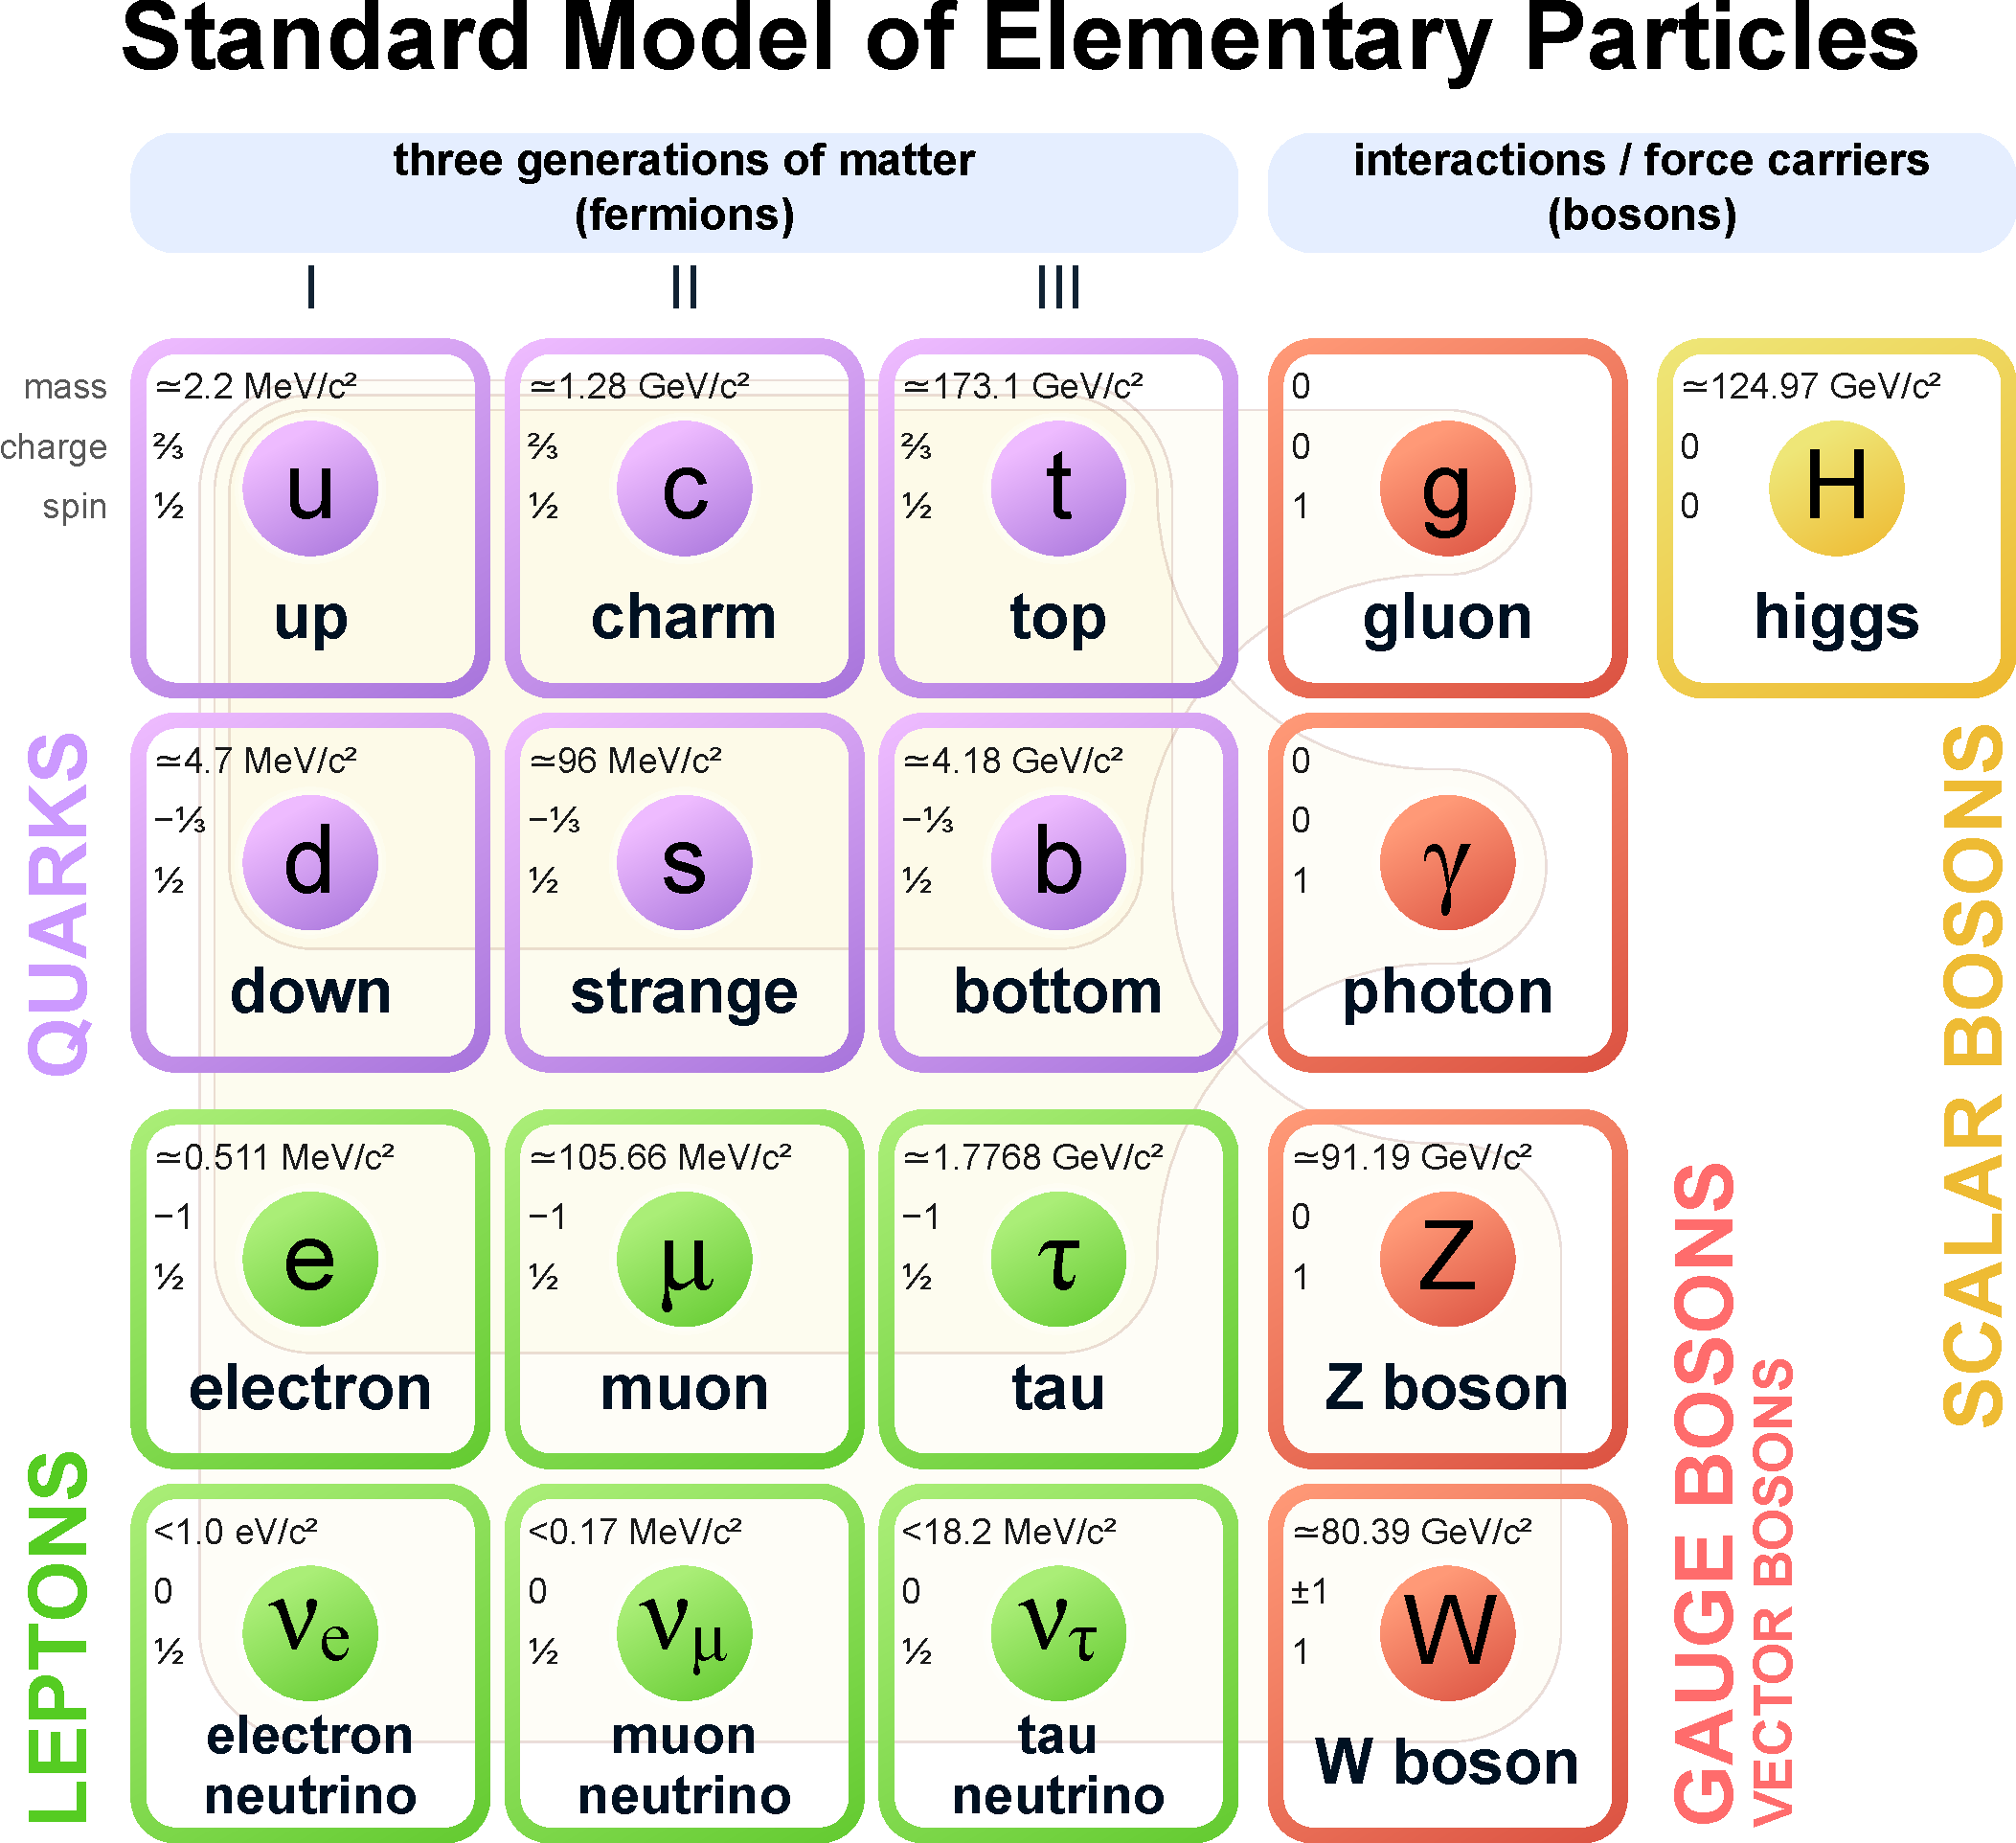
\includegraphics[width=0.6\textwidth]{chap1/Standard_Model_of_Elementary_Particles.pdf}
    \caption{The elementary particles of the Standard Model. Reproduced from
             Wikimedia~\cite{standard_model_wikimedia}.
            }
    \label{fig:Standard_Model_of_Elementary_Particles}
\end{figure}

The Thomas Jefferson National Accelerator Facility (JLab) in Newport News, VA
is home to the Continuous Electron Beam Accelerator Facility (CEBAF).
The CEBAF beam delivers a 12 GeV beam of polarized electrons to four
experimental halls.
Most JLab experiments study the debris produced when the CEBAF electron beam
hits a fixed nuclear target.
By studying this debris, physicists are able to obtain new insights into
nuclear and nucleon structure, exotic configurations of quarks, and other
facets of QCD.

\subsubsection{Scattering in classical physics}
Now what exactly is “quasielastic scattering”?
Elastic scattering is something you might be familiar with from introductory
physics courses.
In Newtonian physics, an elastic collision is one in which kinetic energy is
conserved.
A canonial example is an air hockey puck hitting another puck on a frictionless
plane.
An inelastic collision is one in which kinetic energy is not conserved.
A canonical example is two wads of gum colliding and sticking together in zero
gravity.

\subsubsection{Scattering in nuclear physics}
In nuclear physics, the canonical example of elastic collisions is an electron
colliding with a free proton.
The collision is elastic in the sense that the incoming and outgoing particles
all retain their “identities.”

One of the fun aspects of quantum field theory comes from the intersection of
quantum mechanics and relativity.
Energy and matter are in some sense interchangeable, so some of the energy
contained in colliding particles can be converted into mass.
This is how collisions of proton beams at the LHC create short-lived particles
like the Higgs boson.

At “low” energies, an electron colliding with a nucleus will kick out a proton
or neutron.
Physicists can use this process to study how tightly bound individual nucleons
are in a particular nucleus.

At higher energies, some of this $E=mc^2$ energy can be converted into “new”
particles.
Instead of nucleons, particles like pions, kaons, and muons come out of the
collision.
At this energy scale, we start probing sub-nucleon structures instead of
nuclear structures.
Physicists call these types of interactions “deep inelastic scattering” because
we are using scattering processes to study the “deep” structure of strongly
interacting matter.

Quasielastic scattering is a “low” energy process where the collision looks
like the elastic case of an electron colliding with a free proton.
None of the energy is converted into “new” particles.
The electron transfers momentum to one of a nucleus’s constituent proton,
removing it from its bound state in the nucleus.
This interaction is called “quasielastic” because it looks more like an
electron hitting a free proton than it does a deep inelastic interaction.


\section{Color Transparency}
Color transparency (CT), a characteristic prediction of QCD, refers to the
reduction of initial and final state interactions between a hadron and the
nuclear medium in exclusive processes at large momentum transfer $Q^2$.
The concept was first proposed by Mueller and Brodsky in the context of
perturbative QCD, but was later shown to arise in nonperturbative models.
An analogue of CT can be seen in QED--a small $e^+e^-$ pair has a small cross
section determined by its dipole moment.


The three requirements for CT are the following:
\begin{itemize}
    \item Squeezing: the formation of a small configuration of quarks, sometimes
          referred to as a point-like configuration (PLC)
    \item This PLC is color-neutral outside its radius
    \item Freezing: the PLC maintains its small size over a distance comparable
          to or greater than the nuclear radius
\end{itemize}
There is theoretical support for selection of PLCs in exclusive processes.
Strength of interaction is proportional to transverse size of hadron interacting
with the nuclear medium.
Freezing time can be approximated and has been studied.
Moreover, CT is a necessary condition for the validity of QCD factorization
theorems.


Previous experiments looking for the onset of CT have been suggestive of the
meson electro/photoproduction
A(p,2p) at BNL
A(e,e'p) at SLAC and JLab


In quasielastic scattering experiments, a common observable is the nuclear
transparency $T=\sigma_A/A\sigma_0$, the ratio of the nuclear cross section per
nucleon to the cross section for a free nucleon.
Traditional Glauber multiple scattering theory predicts that $T$ is constant as
$Q^2$ increases.
The reduction of initial/final state interactions predicted by CT results in an
increase in nuclear transparency with $Q^2$.
An illustration of this behavior is shown in Fig~\ref{fig:CT_toy_prediction}.

\begin{figure}[!h]
    \centering
    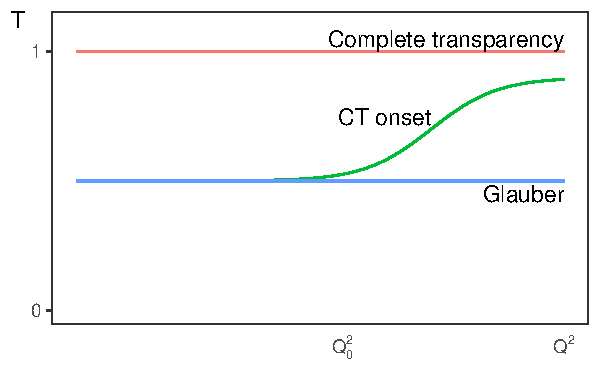
\includegraphics[width=0.8\textwidth]{chap1/CT_toy_prediction.pdf}
    \caption{
            An illustration of the $Q^2$ dependence of nuclear transparency $T$
            for three scenarios.
            The blue line illustrates the prediction of the Glauber model,
            which has constant $T$ as $Q^2$ increases.
            The red line illustrates that for full color transparency, $T=1$;
            in this scenario there are no final state interactions between the
            ejected proton and the rest of the nucleus.
            The green line illustrates the scenario where the transparency
            begins to deviate from the Glauber prediction above an onset
            $Q_0^2$ and approach $T=1$ with increasing $Q^2$.
            }
    \label{fig:CT_toy_prediction}
\end{figure}

Previous measurements of nuclear transparency in quasielastic electron
scattering experiments have been consistent with the Glauber prediction.
The goal of this experiment was to extend the range of $Q^2$ studied
in quasielastic ${}^12C(e,e'p)$ scattering in hopes of observing the onset
of CT.
Data were taken in Hall C at the Thomas Jefferson National Accelerator Facility
in Newport News, VA, using the High Momentum Spectrometer (HMS) and new Super
High Momentum Spectrometer (SHMS) in coincidence.
Data were taken with carbon foil and liquid hydrogen targets over a range of
momentum transfer $Q^2$ from 8.0 to \SI{14.2}{\giga\electronvolt\squared}.


Chapter 2 contains an overview of theoretical considerations relevant to
the experiment and a brief history of previous experiments that studied color
transparency.
Chapters 3 and 4 describe the experimental apparatus and data analysis
procedure.
Chapter 5 contains the final measurements of nuclear transparency and missing
energy and momentum.
Chapter 6 is a conclusion and summary.

\section{Plane Wave Impulse Approximation (PWIA)}

Let $E$ and $E'$ be the incoming and outgoing energies of an electron
scattering elastically from a proton.
The cross section for this process, calculated for single photon exchange,
is given by the Rosenbluth formula
\begin{equation}
\frac{d\sigma}{d\Omega} = \left( \frac{d\sigma}{d\Omega} \right)_{Mott}
                          \frac{E'}{E}
                          \left(
                                \frac{G_E^2 + \tau G_M^2}{1+\tau} +
                                2 \tau G_M^2 \tan^2 \frac{\theta}{2}
                          \right)
\end{equation}
where
$G_E$ and $G_M$ are the electric and magnetic form factors,
$q^\mu=(\omega,\vec{q})$ is the 4-momentum transferred to the proton,
$Q^2=-q_\mu q^\mu$ is the momentum transfer squared,
$\tau=Q^2/4M^2$,
and $\left( \frac{d\sigma}{d\Omega} \right)_{Mott}$ is the cross section for
elastic scattering off a structureless point particle,

\begin{equation}
    \left( \frac{d\sigma}{d\Omega} \right)_{Mott} =
                    \frac{\alpha^2 \cos^2 \frac{\theta}{2}}
                         {4E^2 \sin^4 \frac{\theta}{2}}
\end{equation}

Because nucleons bound in nuclear targets are off-shell and the particles
involved can interact with the surrounding nuclear medium, the Rosenbluth model
is not valid.

% TODO: add Feynman diagram for A(e,e'p)
\begin{figure}[H]
    \centering
        \begin{fmffile}{chap1/quasielastic_scattering}
            \setlength{\unitlength}{1cm}
            \begin{fmfgraph*}(8,5)
                \fmfleft{ie,oe}
                \fmfright{iA,oAm1,op}

                \fmflabel{$(E,\vec{p}_e)$}{ie}
                \fmflabel{$(E',\vec{p'}_e)$}{oe}

                \fmflabel{$(E_A,\vec{p}_A)$}{iA}
                \fmflabel{$(E'_p,\vec{p'}_p)$}{op}
                \fmflabel{$(E_{A-1},\vec{p}_{A-1})$}{oAm1}

                \fmf{fermion}{ie,v1,oe}

                \fmf{photon,label=$q_\mu=(\omega,,\vec{q})$}{v1,v3}

                \fmf{dbl_plain_arrow}{iA,v2}
                \fmfblob{16}{v2}
                \fmf{fermion,label=$(E_s,,\vec{p}_p)$}{v2,v3}
                \fmf{dbl_plain_arrow}{v2,oAm1}
                \fmf{fermion}{v3,op}
            \end{fmfgraph*}
        \end{fmffile}
    \vspace{1cm}
    \caption{Feynman diagram for $A(e,e'p)$ scattering in the PWIA.}
    \label{fig:ele_int_conv}
\end{figure}


The plane wave impulse approximation (PWIA) incorporates these complications
with the following assumptions and approximations:
\begin{enumerate}
    \item Individual nucleons interact with the mean field generated by the rest
        of the nucleus, with no current exchanged between nucleons
    \item Free form factors can be used to describe bound nucleons
    \item The electron and proton's initial and final state wavefunctions are
        undistorted plane waves (meaning there are no ISI, FSI, or Coulomb
        distortions)
    \item The outgoing proton absorbed the entire momentum transfer
    \item Single photon exchange is sufficient to describe the interaction
\end{enumerate}

Incorporating off-shell effects, the differential cross section can be
factorized~\cite{Dieperink_1975, DeForest_1983, Frullani_1984}
% 1975 is the review paper of PWIA
% 1983 is the paper that kind of generalizes the 1976 He3 paper
% 1984 is a more recent review that I had trouble finding, found(!), lost, but can't find anymore
\begin{equation} \label{eqn:born_cross_section}
    \frac{d^6 \sigma}{dE_{e'} d\Omega_{e'} dE_{p'} d\Omega_{p'}} = p_{p'} E_{p'} \sigma_{ep} S(E_s, \vec{p}_p)
\end{equation}
where $\Omega_{e'}$ and $\Omega_{p'}$ are the solid angles of the outgoing particles,
$\sigma_{ep}$ is the off-shell $ep$ cross section,
and the spectral function $S(E_s, \vec{p}_p)$ represents the probability of
finding a proton in the nucleus with initial momentum $\vec{p}_p$ and
separation energy $E_s$.
The separation energy is the energy required to remove a proton from the nucleus
to infinity while leaving the recoil nucleus with zero kinetic energy
$T_{A-1}=0$.
In this work, the $ep$ cross section used is DeForest's
prescription~\cite{DeForest_1983} $\sigma^{cc}_1$,
which was initially calculated in Ref~\cite{Dieperink_1976} for quasielastic
scattering from ${}^3He$.
This cross section is set by imposing momentum and energy conservation at the
$\gamma p$ vertex.
% i.e. J dot q = rho omega
The normalization condition, given nuclear charge $Z$, for the spectral
function is
\begin{equation}
\int d^3p_p dE_s S(E_s, \vec{p}_p) = Z
\end{equation}

$E_s$ and $p_p$ can be estimated by measuring missing energy and momentum
\begin{equation}
    E_m = \omega - T_{p'} - T_{A-1}
\end{equation}
\begin{equation}
    \vec{p}_m = \vec{p}_{p'} - \vec{q}
\end{equation}
where the kinetic energy is $T=E-m$.
These measured quantities differ from $E_s$ and $p_p$ due to FSI, radiative
effects, and the spectrometers' finite resolutions.


The cross section in Equation~\ref{eqn:born_cross_section} assumes the recoil
nucles $A-1$ remains in its ground state.
Coincidence data can include events where this is not the case, for
instance where the recoil nucleus is excited or one spectrometer arm is
triggered by a pion.
Data taken at Saclay~\cite{Mougey_1976} for quasielastic scattering from
${}^{12}C$
suggest that a cut on missing energy below $\SI{\sim100}{MeV}$ limits the rates
of the former.
Cutting on missing energy and using cuts on quantities from particle
identification (PID) detectors limits coincidence events other than $ep$.

\section{Simulation}

\section{Nuclear Transparency}
In order to quantify the effects of final state interactions in interactions
such as quasielastic scattering, experiments measure nuclear transparency--the
ratio of
the measured interaction cross section
to
the cross section calculated in the PWIA.
The definition of transparency used in this work is the same as that used by
previous experiments experiments looking for the onset of CT in
${}^{12},C(e,e'p)$,,
\begin{equation} \label{eqn:transparency_definition}
    T(Q^2) = \frac{\int_{V} d^{3} p_{m} d E_{m} Y^{exp }(E_{m}, \vec{p}_{m})}
                  {\int_{V} d^{3} p_{m} d E_{m} Y^{PWIA}(E_{m}, \vec{p}_{m})}
\end{equation}
where $Y^{exp}$ and $Y^{PWIA}$ are charge-normalized yields from experiment and
simulation, integrated over a volume of missing energy and momentum phase space
$V$, defined by the cuts $E_m < \SI{80}{\mega\electronvolt}$ and
$\norm{\vec{p}_m} < \SI{300}{\mega\electronvolt}$.
Nuclear transparency can be thought of as the probability that a struck proton
will exit the nucleus without rescattering from another nucleon.

\section{Glauber Multiple Scattering Theory}
This experiment takes the work of Pandharipande and
Pieper~\cite{Pandharipande_1992} as the null hypothesis against which the onset
of color transparency is to be tested.
This is the same model used in previous measurements of nuclear transparency
for quasielastic scattering. % TODO: cite previous measurements; garrow etc


% TODO: clean this up a lot. This is basically my notes on the paper.
The model starts with the assumption that the differences between cross
sections for free and in-medium nucleon-nucleon scattering arise primarily from
Pauli blocking of final states and effective mass corrections.
Pandharipande and Pieper find good agreement between experimental results and
their model's estimates of the imaginary part of the optical potential in
nuclear matter.
The model uses the
Urbana $\text{v}_{14}+\text{TNI}$ Hamiltonian~\cite{Lagaris_1981_331, Lagaris_1981_349}
and variational method~\cite{Wiringa_1988, Friedman_1981}
to calculate an optical potential $U$ for symmetric nuclear matter.


The dispersion relation $e(k,\rho)$ for nucleons in nuclear matter with density
$\rho$ and real part of the optical potential $U(k,\rho)$ is
\begin{equation}
    e(k,\rho) = \frac{\hbar^2 k^2}{2m} + U(k,\rho)
\end{equation}

The velocity of an in-medium nucleon with momentum $k$ differs from that of a
free nucleon.
The derivative of the dispersion relation gives this velocity and a
definition of the effective mass $m^*$
\begin{equation}
    \frac{1}{\hbar}\frac{de(k,\rho)}{dk}
        = \frac{\hbar^2 k}{m} + \frac{1}{\hbar}\frac{d}{dk}U(k,\rho)
        \equiv \frac{\hbar k}{m^*(k,\rho)}
\end{equation}

% With this velocity $v'$, transition matrix $t'$, and density of states $D'$,
% the in-medium nucleon-nucleon scattering cross section in a volume of size
% $L^3$ can be expressed as
% \begin{equation}
%     \frac{d\sigma}{d\Omega} = \frac{L^3}{v'} \frac{2\pi}{\hbar} |t'|^2 D'
% \end{equation}
% The equivalent expression holds with unprimed quantities for the vacuum cross
% section.
% Assuming the in-medium correlated two-nucleon wave function at small
% interparticle distances is the same as in the vacuum, the transition matrix
% $t'$ can be taken to be $t' \approx t$.
% Using the approximation from Ref~\cite{Krotscheck_1981}, the in-medium density
% of states is
% \begin{equation}
%     D' = D \frac{m^*\left( \sqrt{\frac{1}{2}(k_3^2+k_4^2)}, \rho \right)}{m}
% \end{equation}
% and the in-medium differential cross section is
% \begin{equation}
% \begin{aligned}
%     \frac{d \sigma^{\prime}}{d \Omega}=& \frac{v_{\mathrm{rel}}}{v_{\mathrm{rel}}^{\prime}} \frac{D_{f}^{\prime}}{D_{f}} \frac{d \sigma}{d \Omega} \\
%     =& \frac{\left|\mathbf{k}_{1}-\mathbf{k}_{2}\right|}{m}\left[\left|\frac{\mathbf{k}_{1}}{m^{*}\left(k_{1}, \rho\right)}-\frac{\mathbf{k}_{2}}{m^{*}\left(k_{2}, \rho\right)}\right|\right]^{-1} \\
%     & \times \frac{m^{*}\left[\sqrt{\left(k_{3}^{2}+k_{4}^{2}\right) / 2}, \rho\right]}{m} \frac{d \sigma}{d \Omega}
% \end{aligned}
% \end{equation}

The in-medium cross section for a proton with momentum $k$ scattering off a
nucleon $a=n,p$ is
\begin{equation}
    \widetilde{\sigma}_{pa}(k,\rho)=\frac{m^{*}(k, \rho)}{\hbar k \rho_{a} \tau_{a}(k)}
\end{equation}
where $\tau_a$ is the life time of the two-particle-one-hole state.
With this expression for the cross section, the nuclear transparency $T$ can be
calculated using a local density approximation and a wavefunction from
conventional Glauber multiple-scattering theory,
\begin{equation}
    T=\frac{1}{Z} \int d^3r' \rho_{p}(\vec{r'}) P_{T}(\vec{r'})
\end{equation}
where $P_T$, the probability that a proton struck at $\vec{r'}$ emerges without
rescattering, is

% with align
\begin{equation}
\begin{aligned}
    P_{T}(\vec{r'}) = \exp \biggl\{-\int_{z'}^{\infty} dz'' \biggr.\biggl[&g_{p n}(\vec{r'}, \vec{r''}) \widetilde{\sigma}_{p n}\left(k, \rho(\vec{r''})\right) \rho_{n}(\vec{r''})\biggr.\\
                                                           \biggl.\biggl.+&g_{p p}(\vec{r'}, \vec{r''}) \widetilde{\sigma}_{p p}\left(k, \rho(\vec{r''})\right) \rho_{p}(\vec{r''})\biggr]\biggr\}
\end{aligned}
\end{equation}

% % one long line
% \begin{equation}
%     P_{T}(\vec{r'}) =
%     \exp \left\{
%         -\int_{z'}^{\infty} dz'' \left[
%             g_{pn}(\vec{r'},\vec{r''})\widetilde{\sigma}_{pn}(k, \rho(\vec{r''})) \rho_{n}(\vec{r''})
%             +
%             g_{pp}(\vec{r'},\vec{r''})\widetilde{\sigma}_{pp}(k, \rho(\vec{r''})) \rho_{p}(\vec{r''})
%         \right]
%     \right\}
% \end{equation}

In the above expression, $g_{pa}(\vec{r'},\vec{r''})$ is a pair distribution
function~\cite{Schiavilla_1987}, the joint probability to find a proton at
$\vec{r'}$ and nucleon $a$ at $\vec{r''}$.

% TODO: elaborate on why this predicts constant T?

\section{The Onset of Color Transparency}
The signature of the onset of CT is a rise in $T$ with $Q^2$ above some
threshold $Q^2_0$.
Previous measurements of T in ${}^{12}C(e,e'p)$ at SLAC, MIT-Bates, and JLab
for momentum transfers between $Q^2=0.6$ and
\SI{8.1}{\giga\electronvolt\squared} have been consistent with the predictions
of the Glauber model.

The model presented by Frankfurt et al.~\cite{Frankfurt_1995_PRC} starts by
calculating the amplitude $\mathcal{M}_{h}^{\gamma^*A}$ for quasielastic
scattering of a proton from a fixed shell $h$ in a nucleus.
This amplitude includes the effects of short range nucleon-nucleon
correlations, both between the ejected proton and remainder nucleons in the
recoil nucleus as well as between the remainder nucleons.
Using the distorted wave impulse approximation (DWIA), they derive an
expression for nuclear transparency whose behavior is dependent on the form of
nucleon-nucleon interactions.
These interactions are parameterized by profile functions $\Gamma(\vec{b})$
that are a function of impact parameter $\vec{b}$.
They compare two choices of profile function--one which corresponds to the
absence of CT and one which includes a model of CT in which~\cite{Farrar_1988}
the PLC grows to the full size of a proton over a length $l_h$, the hadron
formation length.


The model presented by Cosyn et al.~\cite{Cosyn_2008,Cosyn_2006} uses a
relativistic multiple scattering Glauber approximation~\cite{Ryckebusch_2003}
that accounts for final state interactions by applying a phase to the ejected
proton's wavefunction.
This phase is determined by a profile function $\Gamma(\vec{b})$ that
parameterizes nucleon-nucleon scattering.
As in the other model, this profile function is modified to include CT effects
Short range correlations are implemented by means of an effective nucleon
density~\cite{Frankel_1994} that enters into the calculation of the Glauber
phase.


To include CT effects, both models replace the total cross section
$\sigma_{tot}$ with an effective cross section $\sigma_{eff}$
based on a quantum diffusion model~\cite{Farrar_1988}
that accounts for reduced interaction between the prehadron and nuclear matter
over a hadron formation length $l_h$,
\begin{equation}
    \sigma_{eff} = \sigma_{tot}
    \left\{
        \left[\frac{z}{l_h} +
               \frac{\left\langle n^{2} k_{t}^{2}\right\rangle}{t} \left(1-\left(\frac{z}{l_h}\right)\right)
        \right]
        \theta\left(l_h-z\right) +
        \theta\left(z-l_h\right)
    \right\}
\end{equation}
In this expression,
$n$ is the number of valence quarks (2 for mesons, 3 for baryons),
$k_t \sim \SI{1}{\giga\electronvolt\squared}/Q^2$
is the average transverse momentum of a quark inside a hadron,
$z$ is the distance the object has traveled since its creation,
and
$l_h=2p/\Delta M^2$ is the hadronic formation length.
This length depends on
the momentum $p$ of the outgoing hadron
and
the mass squared difference between the prehadron and outgoing hadron state.
Frankfurt et al. use $\Delta M^2 = \SI{0.7}{\giga\electronvolt\squared}$
for protons, while
Cosyn et al. use $\Delta M^2 = \SI{1.0}{\giga\electronvolt\squared}$.

\subsection{Frankfurt et al.}

% Frankfurt et al. derive an modified nuclear density $\tilde{\rho}(r)$ that
% takes nucleon correlations into account based on single nucleon density
% functions $\rho(r)$ and two-body correlation functions $g_h(r,r')$,
% \begin{equation}
%     \tilde{\rho}(r)
%         = (A-1) \rho(r)
%           \left[
%                1 + C_h(r_1,r) - \frac{A-1}{2} \int_{z_1} \Gamma(b_1-b')g_h(r,r')\rho(r')d^3r'
%           \right]
% \end{equation}
% Here, $C_h(i,j)$ are two-nucleon correlation factors that are functions of the
% distance $r_{ij}=|\vec{r}_j-\vec{r}_i|$ between nucleons $i$ and
% $j$~\cite{Weise_1972}.
% The single nucleon wave functions $\phi_h(r)$ are the overlap integral between
% wave functions of the $A$-body ground state wave function and the $(A-1)$-body
% recoil nucleus.
% Their normalization requires $\int|\phi_h(r)|d^3r=1$ and
% $\rho(r) = \sum_h \omega_h^2 \left| \phi_h(r) \right|$ where $\omega_h$ is the
% occupation probability of the orbital $h$.

% \begin{equation}
%     \mathcal{M}_{h}^{\gamma^*A} = \int d^3 r_1 \omega_h \phi_h\left(r_{1}\right)
%                                   \hat{O}^{\mathrm{em}}\left(Q^{2}\right)
%                                   e^{-i \vec{p}_p \cdot \vec{r}_1}
%                                   \exp{- \int_{z_{1}}
%                                   \Gamma\left(b_{1}-b\right) \tilde{\rho}(r) d^3 r}
% \end{equation}

In the DWIA, the cross section can be written
\begin{equation}
    \frac{d^6\sigma}{dE'_{e} d\Omega'_{e} d^3p'_{p}} = p'_p E'_p \sigma_{eN} S(\vec{p}_p, E_M, \vec{p'}_p)
\end{equation}
where $\sigma_{eN}$ is the cross section for an electron scattering from a
bound nucleon and $S(\vec{p}_p, E_M, \vec{p'}_p)$ is the distorted
spectral function.
For a fixed shell $h$ the spectral function can be written~\cite{Frullani_1984},
\begin{equation}
    S(\vec{p}_p, E_M, \vec{p'}_p) = n_h(E_m) |\Phi_h(\vec{p}_p, \vec{p'}_p)|^2
\end{equation}
where $\Phi_h(\vec{p}_p, \vec{p'}_p)$ is the distorted momentum distribution for
nucleons in the $h$ shell
and
$n_h(E_m)$ (proporitonal to the shell's occupation probability) characterizes
the strength of the shell.
Frankfurt et al. derive the following expression for the momentum distribution
by expressing the ground state $A$-body wave function and $(A-1)$-body density
matrix in terms of two-nucleon correlation functions
\begin{equation}
    \left| \Phi_h(\vec{p}_p, \vec{p'}_p)\right|^2
        = \left|
            \int d^3 r_1 \Psi_h(r_1) e^{-i \vec{p}_p \cdot \vec{r}_1}
            \exp{\left\{- \int_{z_{1}} \Gamma\left(\vec{b}_1-\vec{b}\right) \tilde{\rho}(r) d^3 r\right\}}
          \right|
\end{equation}

The profile function $\Gamma(\vec{b})$ takes the form
\begin{equation}
    \Gamma(\vec{b}) = \frac{1}{2\pi i k}
                  \int e^{i\vec{k}_t \cdot \vec{b}} f(\vec{k}_t) d^2k_t
\end{equation}
where the nucleon-nucleon scattering amplitude with CT effects is
\begin{equation}
    f_{CT}(k_t, z, Q^2) = i\frac{k}{4\pi} \sigma_{eff}(z,Q^2) e^{Bt/2}
                          \frac{G_N\left( t \sigma_{eff}(z,Q^2)/\sigma_{eff} \right)}
                               {G_N\left( t \right)}
\end{equation}
and the amplitude without CT effects is
\begin{equation}
    f(k_t) = \left(\frac{k_t}{4\pi}\right)^2
             \sigma_{tot}^2
             (1+\epsilon^2) e^{-Bt}
\end{equation}
%All prameters are taken from their refs 29-31
where
$\epsilon$ is the ratio of the scattering amplitude's real and imaginary parts
and
$B$ is a slope parameter.

The nuclear transparency for the $h$ shell is the ratio of the distorted
momentum distributions from the DWIA and PWIA,
\begin{equation}
    T_h = \left(\frac{\sigma^{exp}}{\sigma^{PWIA}}\right)
        = \frac{|\Phi^{DWIA}_h(p_p,p'_p)|^2}
               {|\Phi^{PWIA}_h(p_p)|^2}
\end{equation}

Transparency predictions for ${}^{12}C(e,e'p)$ scattering from the $s$ shell,
with and without CT, are shown in Fig~\ref{fig:frankfurt_transparency}.

% The ground state wavefunctions Frankfurt et al. use are calculated in the
% Skyrme-Hartree-Fock model with correlated interactions~\cite{Reinhard_1991}.

\begin{figure}[h]
    \centering
    \begin{subfigure}[b]{0.45\textwidth}
        \centering
        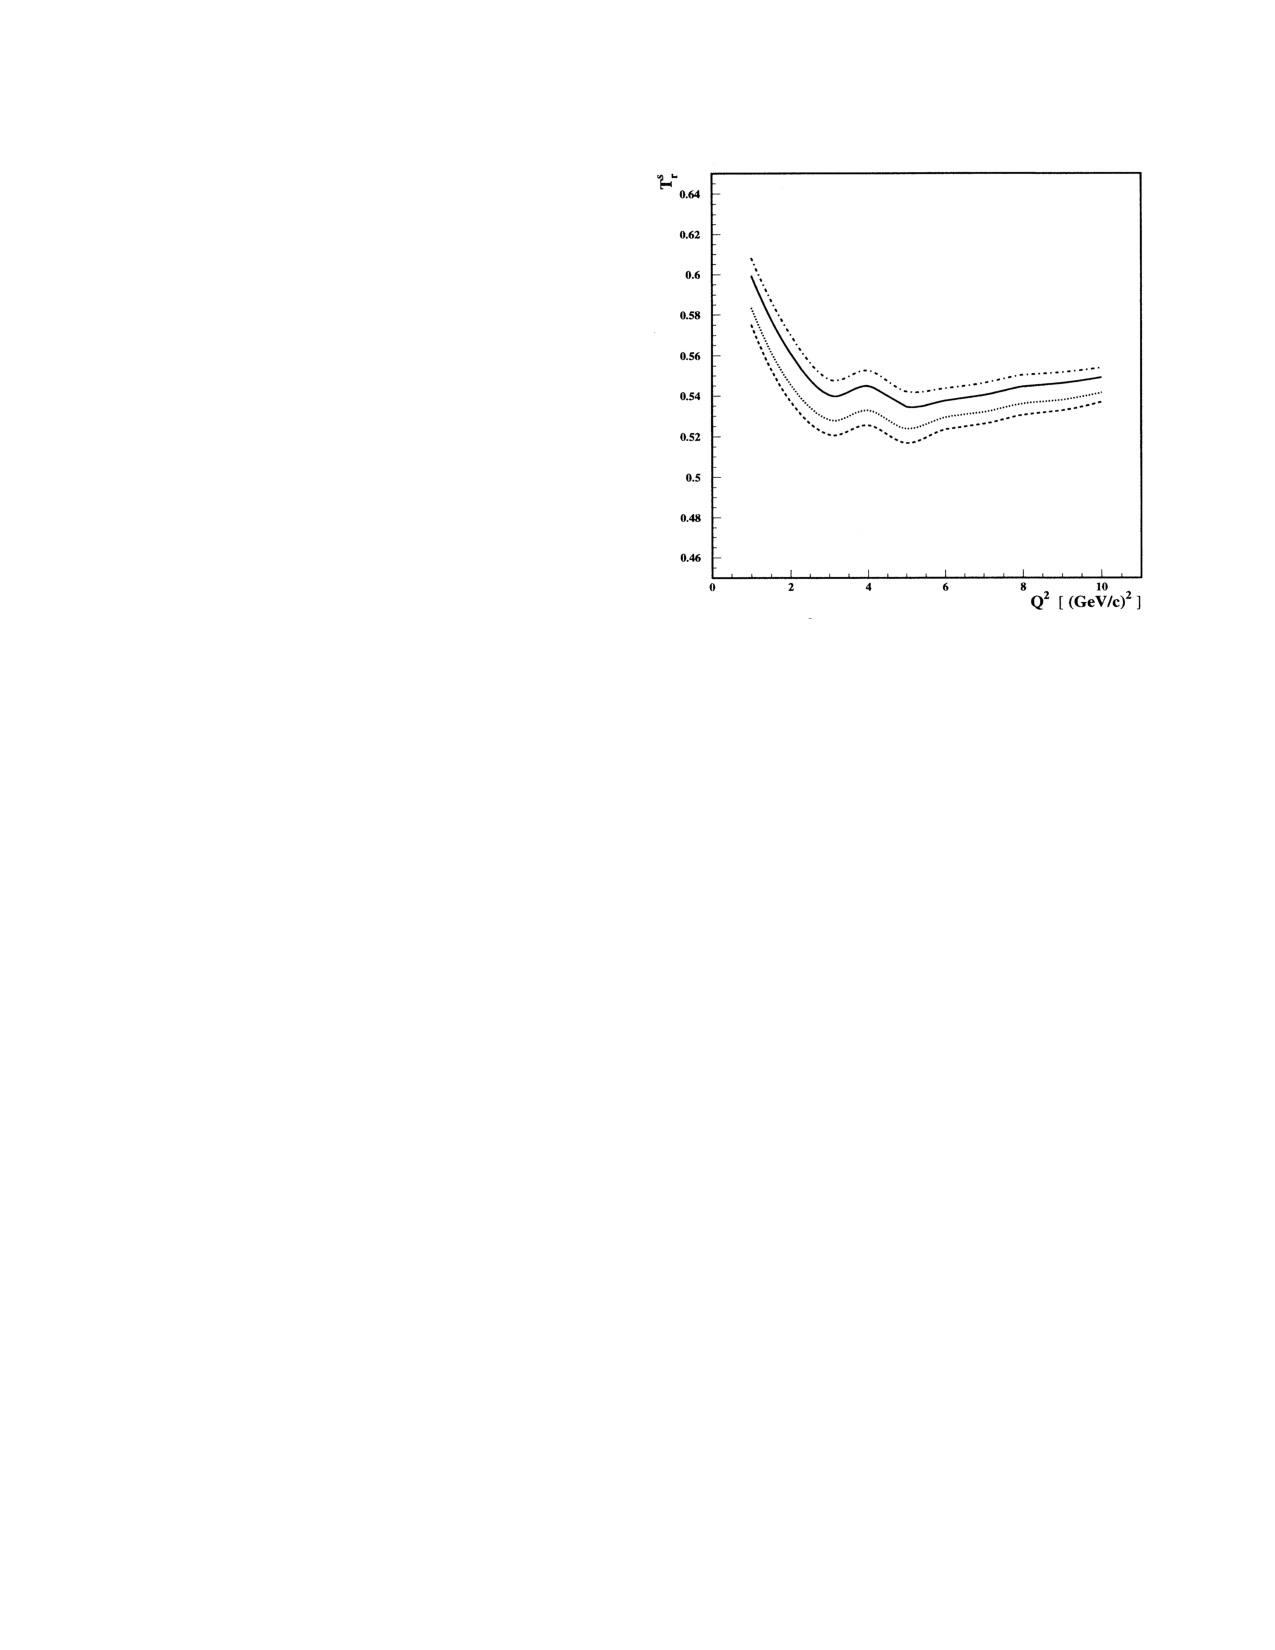
\includegraphics[width=\textwidth]{chap1/frankfurt_transparency_without_CT.pdf}
        % \caption{X plane}
        \label{fig:frankfurt_transparency_without_CT}
    \end{subfigure}
    % \hfill
    \begin{subfigure}[b]{0.45\textwidth}
        \centering
        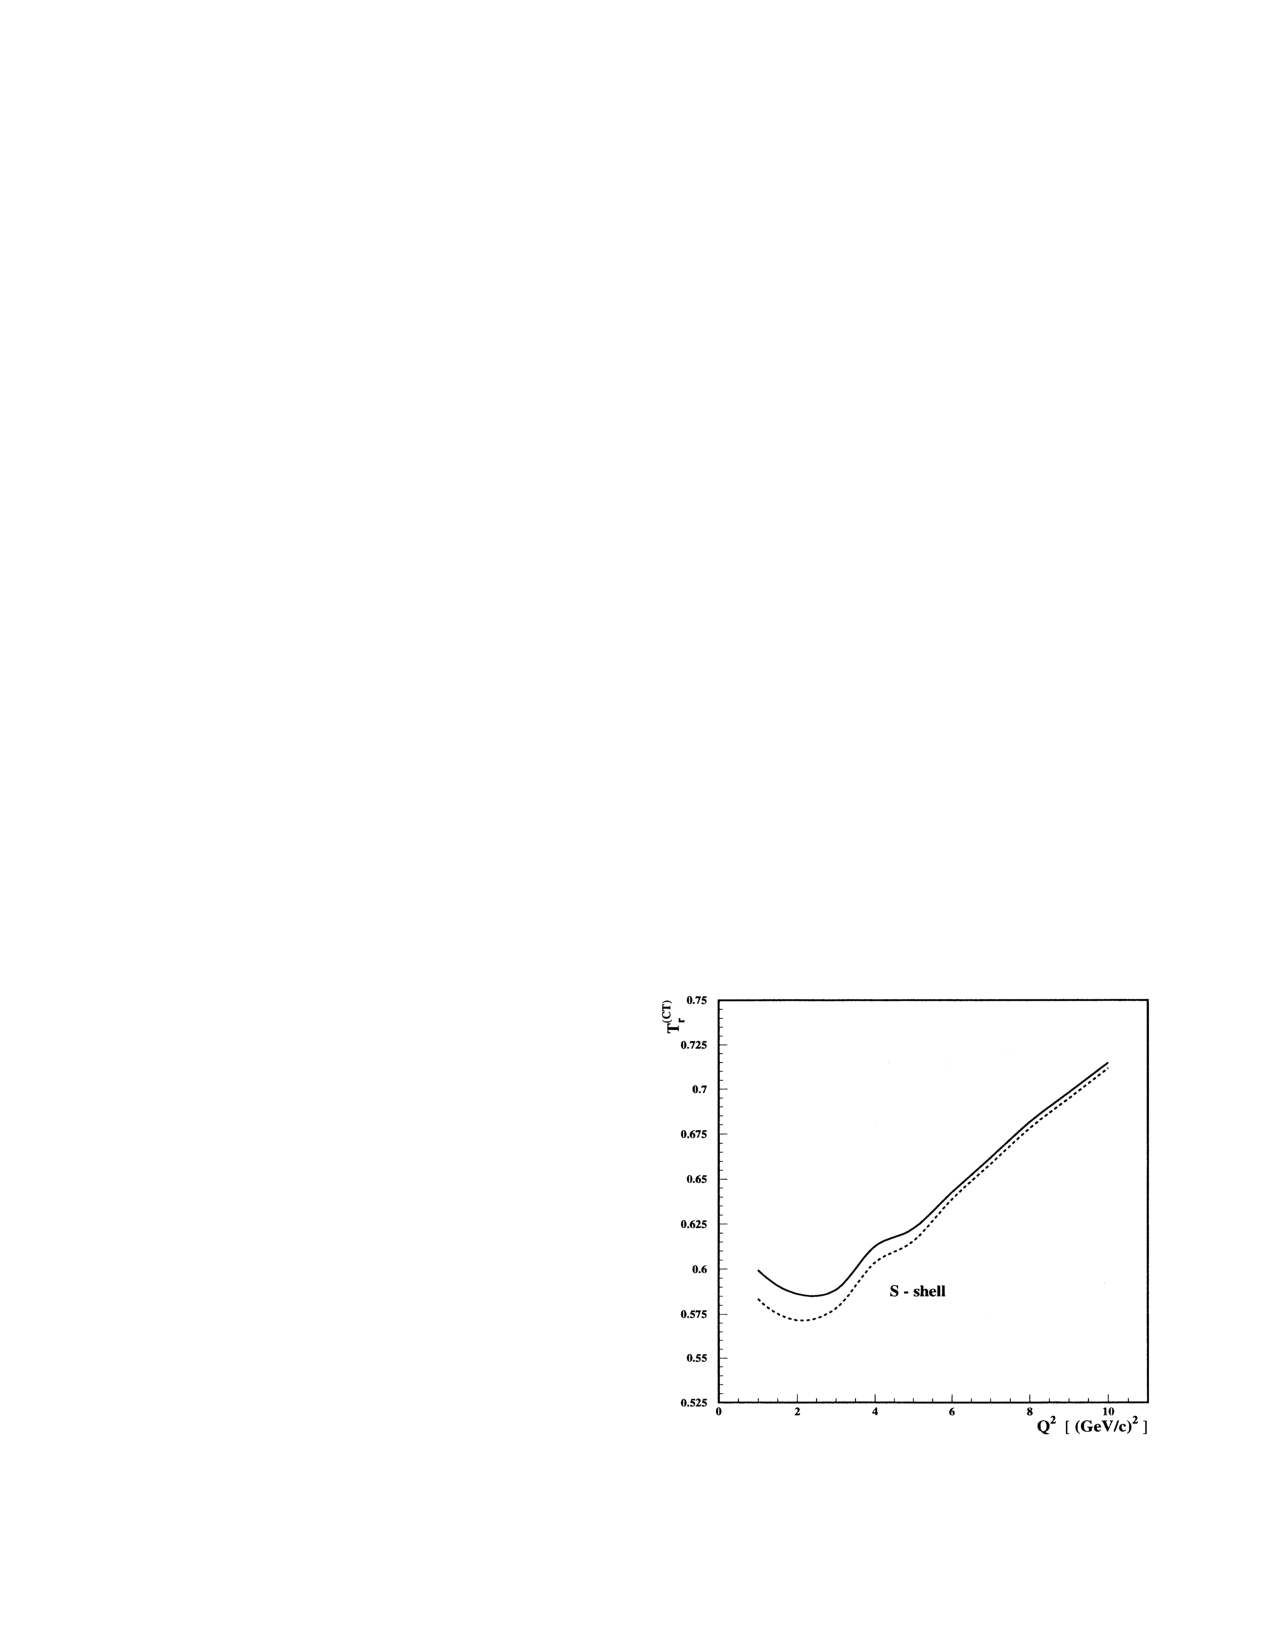
\includegraphics[width=\textwidth]{chap1/frankfurt_transparency_with_CT.pdf}
        % \caption{U plane}
        \label{fig:frankfurt_transparency_with_CT}
    \end{subfigure}
    \caption{Transparency calculations for ${}^{12}C(e,e'p)$ based on a model
             that accounts for nucleon correlations and proton knock-out from
             particular nuclear shells~\cite{Frankfurt_1995_PRC}.
             The figure on the left is for a model that does not include CT.
             The dotted line is the calculation without correlation effects;
             the dashed line, with the effects of correlation between undetected nucleons;
             the dash-dotted line, with the effects of correlation between knocked-out proton and undetected nucleons;
             and solid line, with over-all correlation effects.
             The figure on the right includes CT.
             The dashed line is the calculation without correlation effects;
             the solid line, with corrleation effects.
             The rise in transparency with $Q^2$ is the characteristic
             signature of the onset of CT.
             Note that the effect of nucleon correlations on the CT model is
             a correction of a few percent.
             }
    \label{fig:frankfurt_transparency}
\end{figure}



\subsection{Cosyn et al.}

The model of Cosyn et al. derives eikonal approximation of equation~\ref{eqn:eikonal_approximation}.
After rescattering, the outgoing wavefunction $\psi_{out}$ picks up a complex
phase $\chi(\vec{r})$.
\begin{equation}
    \psi_{out}(\vec{r}) = e^{i\chi(\vec{r})} \psi_{in}(\vec{r})
\end{equation}

This phase can be parameterized as a function of impact parameter $\vec{b}$,
momentum transfer $Q^2$, etc. by a profile function $\Gamma(\vec{b})$.
For a single rescattering,
\begin{equation}
    \psi_{out}(\vec{r}) = (1-\Gamma(\vec{b})) \psi_{in}(\vec{r})
\end{equation}

Every spectator nucleon in the recoil nucleus lying in the forward path of the
ejected proton contributes to the total phase.
Let $\vec{r}$ be the point at which the ejected proton absorbs the virtual
photon.
The total phase shift for $A$ nucleons is a product
\begin{equation}
    e^{i\chi(\vec{r})} = \prod_{j=2}^{A} \left(1-\Gamma(\vec{b}_j)\theta(z_j-z)\right)
\end{equation}

The profile function for a hadron $h$ scattering from a nucleon $N$ is
determined by
the interaction cross section $\sigma^{hN}_{tot}$,
the ratio $\epsilon_{hN}$ of the scattering amplitude's real and imaginary parts,
and slope parameter $\beta_{hN}$,
all of which are momentum-dependent.
These parameters can be estimated by interpolating data from the Particle Data
Group.
\begin{equation}
    \Gamma(\vec{b}) =
        \frac{\sigma^{hN}_{tot}(1-i\epsilon_{hN})}
             {4\pi\beta_{hN}^2}
        \exp{-\frac{\vec{b}^2}{2\beta_{hN}^2}}
\end{equation}

The slope parameter $\beta_{hN}$ can be estimated using
the elastic $\sigma^{hN}_{el}$ and total $\sigma^{hN}_{tot}$ cross sections
in the following
approximation~\cite{Ryckebusch_2003}
\begin{equation}
    \beta_{p N}^{2} \approx
            \frac{(\sigma^{hN}_{tot})^{2} (\epsilon_{hN}^{2}+1)}
                 {16 \pi \sigma^{hN}_{el}}
\end{equation}



\chapter{Theoretical Overview}


\chapter{Experimental Apparatus}

\section{Overview}
\lipsum[1-2]

\section{Accelerator}
\lipsum[1-2]

\subsection{CEBAF}
\lipsum[1-2]

\subsection{Beam Position Monitors}
\lipsum[1-2]

\subsection{Beam Current Monitors}
\lipsum[1-2]

\subsection{Beam Rastering System}
\lipsum[1-2]

\section{Targets}
The target chamber is a large evacuated cylinder located above the
spectrometers' pivot point, designed to allow each spectrometer to rotate
around it without any coupling between the beam line vacuum and the
spectrometers' vacuum.
Figure~\ref{fig:target_chamber} is a rendering of the target chamber, viewed
from the exit window and beam exit pipe.
A single target ladder, a rendering of which can be found in
Figure~\ref{fig:target_ladder} containing solid and cryogenically cooled liquid
targets can be raised or lowered via a GUI in the counting house to select a
desired target.

\begin{figure}[h]
    \centering
    \begin{subfigure}[b]{0.4\textwidth}
        \centering
        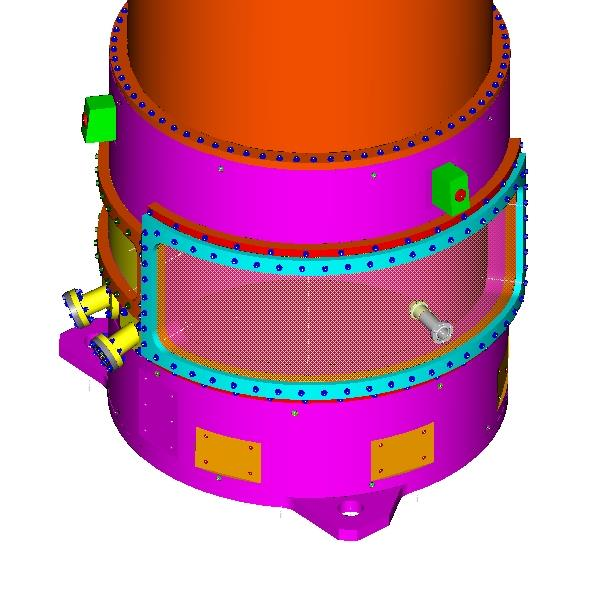
\includegraphics[width=\textwidth]{chap3/target_chamber.jpg}
        % \caption{X plane}
        \label{fig:target_chamber1}
    \end{subfigure}
    % \hfill
    \begin{subfigure}[b]{0.4\textwidth}
        \centering
        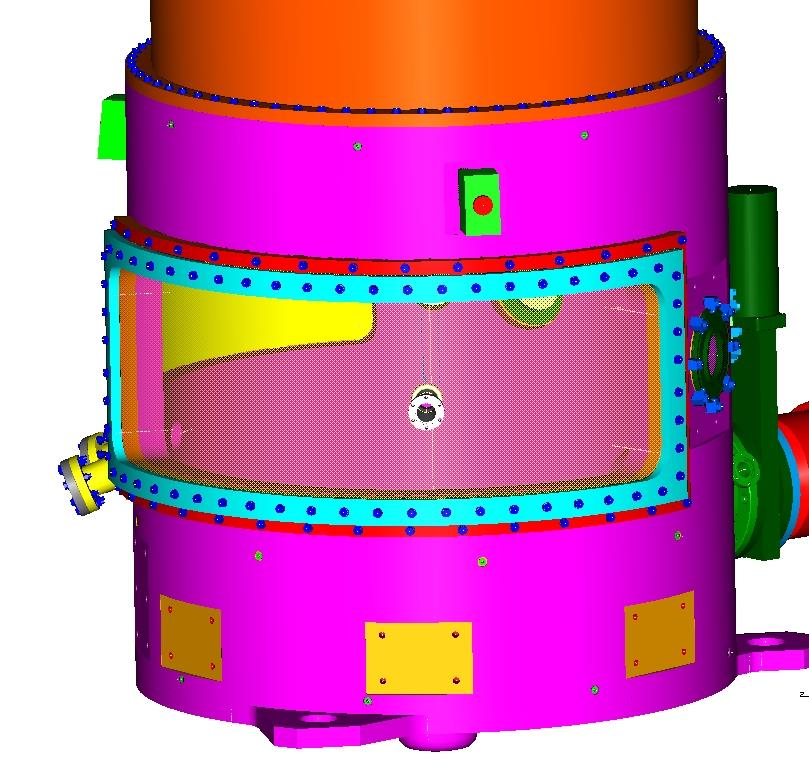
\includegraphics[width=\textwidth]{chap3/target_chamber2.jpg}
        % \caption{U plane}
        \label{fig:target_chamber2}
    \end{subfigure}
    \caption{The Hall  C target chamber.
             }
    \label{fig:target_chamber}
\end{figure}

\begin{figure}[h]
    \centering
    \begin{subfigure}[t]{0.3\textwidth}
        \centering
        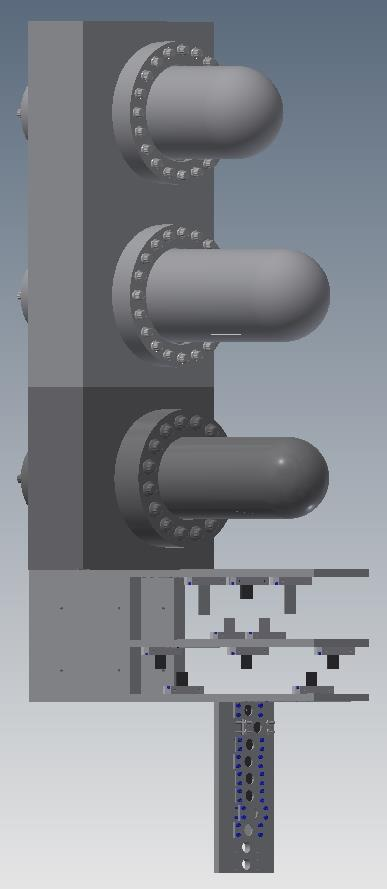
\includegraphics[height=3.5in]{chap3/target1.jpg}
        % \caption{}
        \label{fig:target_ladder1}
    \end{subfigure}
    \hfill
    \begin{subfigure}[t]{0.3\textwidth}
        \centering
        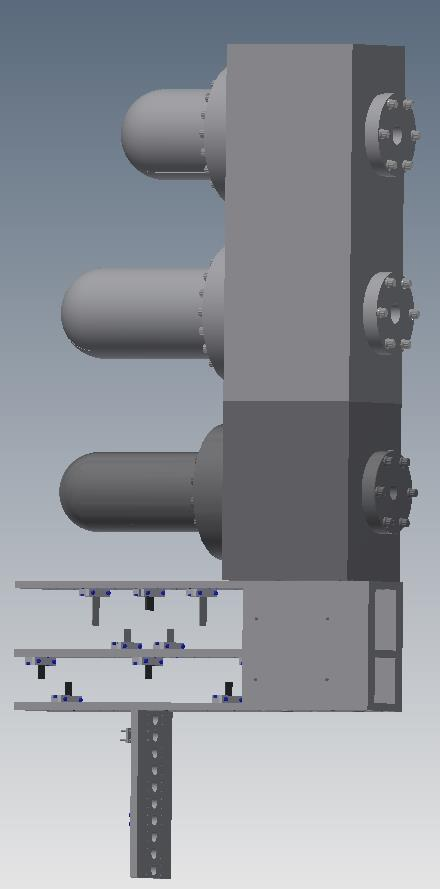
\includegraphics[height=3.5in]{chap3/target2.jpg}
        % \caption{}
        \label{fig:target_ladder2}
    \end{subfigure}
    \hfill
    \begin{subfigure}[t]{0.3\textwidth}
        \centering
        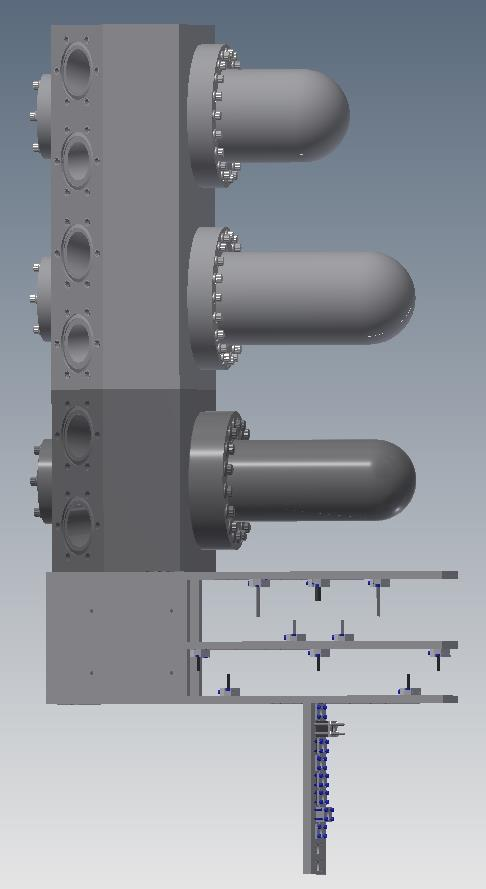
\includegraphics[height=3.5in]{chap3/target3.jpg}
        % \caption{}
        \label{fig:target_ladder3}
    \end{subfigure}
    \caption{The Hall C target ladder.
             }
    \label{fig:target_ladder}
\end{figure}

The target ladder contains three cryotarget loops, two ``dummy'' targets
consisting of two aluminum foils placed at z positions corresponding to the
entrance and exit windows of the cryotargets, two optics targets, and a number
of solid targets.
Table~\ref{tab:target_ladder_summary} summarizes the target ladder as
configured for the 2017 commissioning experiments, including our experiment,
E12-06-107.
During our experiment, cryotarget loop 1 was filled with \ch{LHe3}, loop 2
with \ch{LH2}, and loop 3 with \ch{LD2}.
The loops can be filled with other gases depending on experimental
requirements.

A detailed engineering drawing of the ladder is available online~\cite{target_drawing}.

\begin{table}[h]
    \centering
    \caption{Summary of the materials and thicknesses of the cryotarget loops and dummy targets.}
    \label{tab:target_ladder_summary}
    \begin{subtable}[h]{1.0\textwidth}
        \caption{Cryotarget loops and dummy targets}
        \resizebox{1.0\textwidth}{!}{
            \begin{tabular}[t]{lllll}
                \hline
                \hline
                Target          & Entrance Thickness [mm]  & Exit thickness [mm]     & Length [mm]     & Material  \\
                \hline
                Loop 1 (4 cm)   & $0.165 \pm 0.0019$       & $0.151 \pm 0.0053$ Tip  & $40  \pm 0.25$  & Aluminum 7075   \\ % tip
                                % &                          & $0.151 \pm 0.0097$ Wall &                 &           \\
                                                                                                                   % \\
                Loop 2 (10 cm)  & $0.104 \pm 0.0025$       & $0.133 \pm 0.0096$ Tip  & $10  \pm 0.26$  & Aluminum 7075   \\ % tip
                                % &                          & $0.162 \pm 0.014$ Wall  &                 &           \\
                                                                                                                   % \\
                Loop 3 (15 cm)  & $0.147 \pm 0.008$        & $0.177 \pm 0.013$ Tip   & $150 \pm 0.26$  & Aluminum 7075   \\ % tip
                                % &                          & $0.24  \pm 0.025$ Wall  &                 &           \\
                                                                                                                   % \\
                4 cm dummy      & $0.0789 \pm 0.000148$    & $0.0811 \pm 0.00014$    &                 & Aluminum 7075   \\
                                                                                                                   % \\
                10 cm dummy     & $0.1816 \pm 0.0003$      & $0.1815 \pm 0.0003$     &                 & Aluminum 7075   \\
                (with carbon foil at  & & & & \\
                z=0, described below) & & & & \\
                \hline
            \end{tabular}
            \label{table:target_ladder_cryo_summary}
        } % resizebox
    \end{subtable}
    \vspace{1cm}
    \begin{subtable}[h]{1.0\textwidth}
        \caption{Optics and solid targets}
        \resizebox{1.0\textwidth}{!}{
            \begin{tabular}[t]{llcl}
                \hline
                \hline
                Target                 & Thickness [\si{\g\per\cm\squared}] & z position [cm] & Material  \\
                \hline
                Optics (three foils)   & $0.044  \pm 0.001$                  & -10, 0, +10     & Aluminum 7075/Carbon 99.95\%                         \\
                Optics (two foils)     & $0.044  \pm 0.001$                  & -5, +5          & Carbon 99.95\%                                       \\
                Carbon on 10 cm dummy  & $0.4426 \pm 0.0008$                 & 0               & Carbon 99.95\%                                       \\
                Carbon Hole            & $0.171  \pm 0.001$                  & 0               & Carbon 99.95\%                                       \\
                Carbon 6\%             & $2.068  \pm 0.004$                  & 0               & Carbon 99.95\%                                       \\
                Carbon 1.5\%           & $0.5244 \pm 0.001$                  & 0               & Carbon 99.95\%                                       \\
                Carbon 0.5\%           & $0.1749 \pm 0.00035$                & 0               & Carbon 99.95\%                                       \\
                \ch{^{10}B4C}          & $0.5722 \pm 0.001$                  & 0               & \ch{^{10}B4C} (99.9\% Chem/95\% enrichment)          \\
                \ch{^{11}B4C}          & $0.6348 \pm 0.001$                  & 0               & \ch{^{11}B4C} (99.9\% Chem/95\% enrichment)          \\
                \ch{BeO}               & $0.263  \pm 0.001$                  & 0               & \ch{BeO} 99.5\%                                      \\
                \hline
            \end{tabular}
            \label{table:target_ladder_cryo_summary}
        } % resizebox
    \end{subtable}
\end{table}

Each cryotarget loop is maintained at \si{\sim3}{K} below the fluid's boiling
point by constantly recycling the fluid through a circuit containing the target
cell and a heat exchanger.

% TODO: Modify Greg's figure to reflect new cell geometry
\begin{figure}[!h]
    \centering
    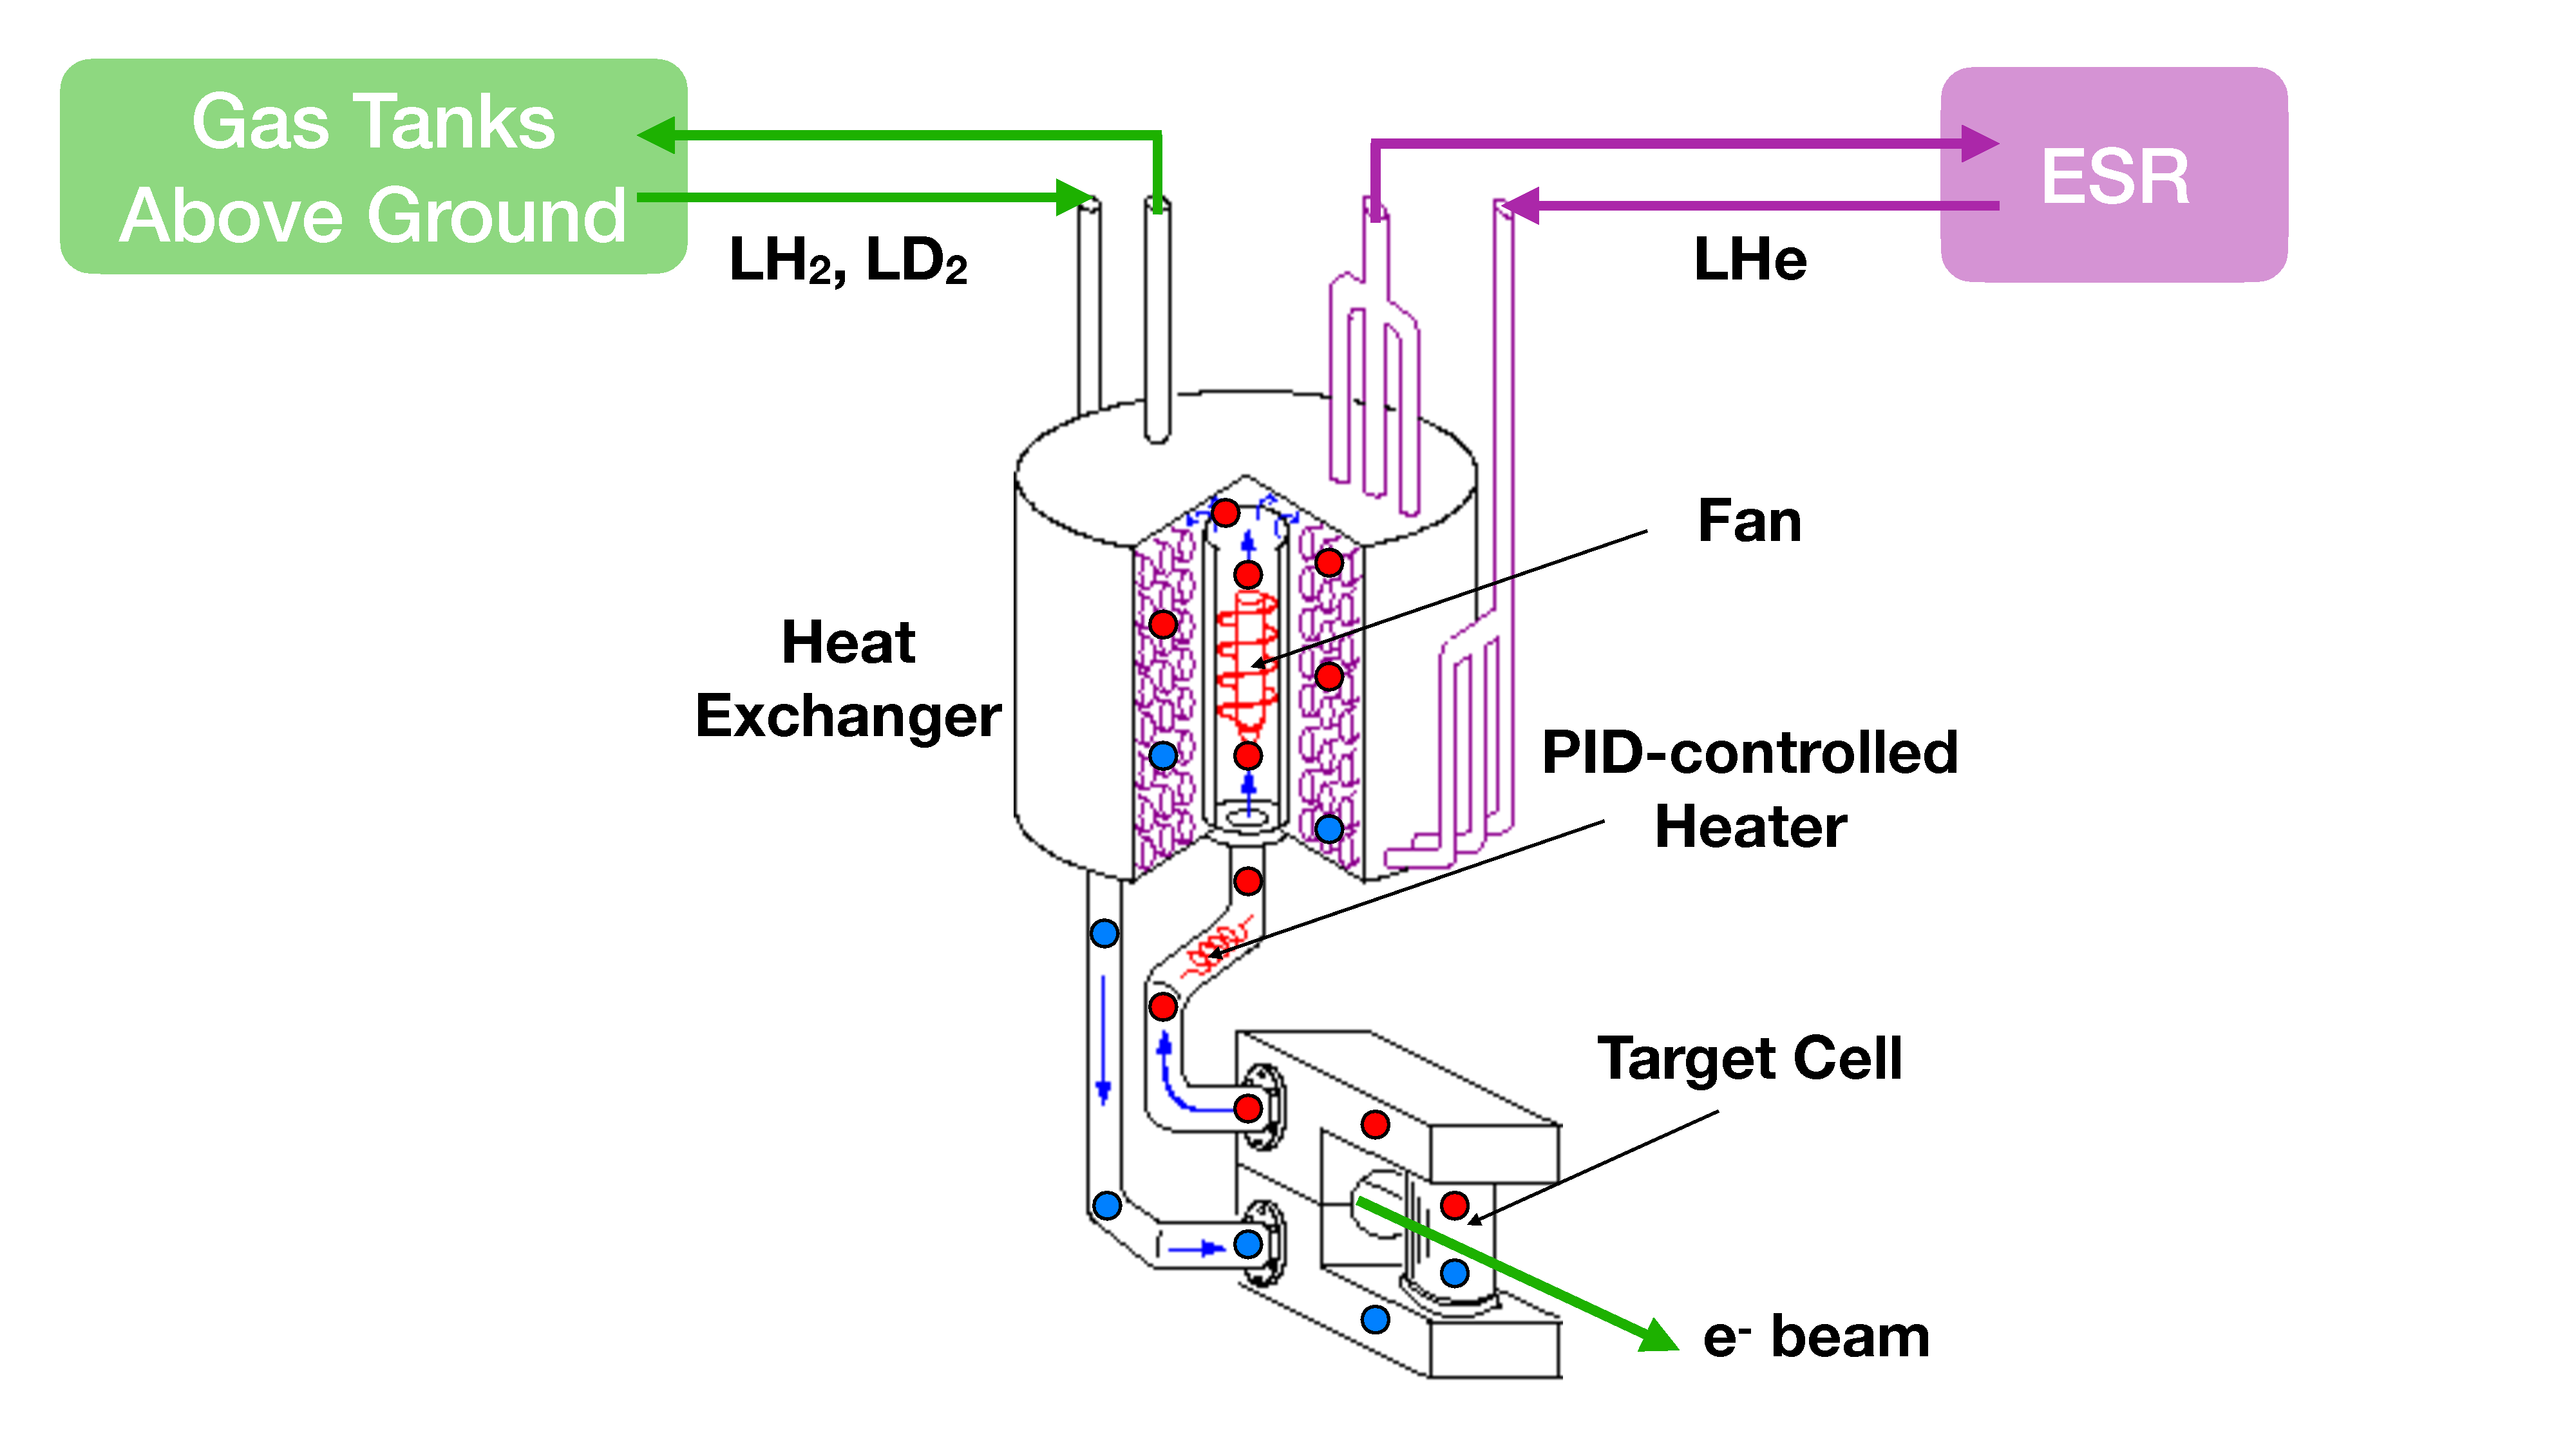
\includegraphics[width=1.0\textwidth]{chap3/target_cell_temperature_control.pdf}
    \caption{A cartoon of the system that maintains the cryotargets'
             temperatures.
            }
    \label{fig:cryotarget_temperature_regulation}
\end{figure}

A gas panel outside the counting house feeds a constant supply of target fluid
to the heat exchanger, where the \si{15}{K} liquid helium coolant from the End
Stage Refrigerator cools it to the target temperature of \si{\sim3}{K} below
boiling.
The fluid is then sent to the target cell which is  designed to maintain
uniform fluid velocity and density as the fluid makes its way from the cell's
inlet to its outlet.
As it leaves, the fluid will be at a higher temperature due to heat deposited
by the beam in operating conditions.
In the event that the beam is off, tripped, or otherwise interrupted, a high
power heater controlled by a software PID (Proportional-Integral-Derivative)
loop heats the exiting target fluid as if the beam were present.
The fluid then returns to the heat exchanger, completing the circuit.

\section{Spectrometers}
The major experimental equipment in Hall C consists of two medium-resolution,
large-acceptance magnetic spectrometers with similar flexible detector
packages.
The High Momentum Spectrometer (HMS) is designed to analyze particles with
momenta up to 7.4 GeV.
The Super High Momentum Spectrometer (SHMS) is designed to analyze particles
with momenta up to 11 GeV.
The spectrometers' detector packages are designed to analyze both electrons
and hadrons in coincidence or single-arm experiments studying inclusive and
exclusive reactions.
Both spectrometers' magnets and detector stacks sit on independent carriages
that rotate on rails around a central pivot located beneth the target chamber.
A summary of the spectrometers' performance is given in table
\ref{tab:spectrometer_performance}.


For E12-06-102's production data, protons were detected in the SHMS in
coincidence with electrons in the HMS.
Additional single-arm data were taken for the purpose of detector calibration.

\begin{table}[h]
    \centering
    \caption{Summary of the HMS performance and design specifications for the SHMS.}
    \label{tab:spectrometer_performance}
    \resizebox{1.0\textwidth}{!}{
        \begin{tabular}[t]{lll}
            \hline
            \hline
            Parameter                            & HMS                            & SHMS                        \\
            \hline
            Central Momentum Range               & 0.4 \textendash 7.4 GeV/c      & 2 \textendash 11 GeV/c      \\
            Momentum Acceptance                  & $\pm10\%$                      & $-10\%$ to $+22\%$          \\
            Momentum Resolution                  & $0.1\%-0.15\%$                 & $0.03\%-0.08\%$             \\
            Scattering Angle Range               & 10.5$^\circ$ to 90$^\circ$     & 5.5$^\circ$ to 40$^\circ$   \\
                                                                                                                \\
            Target Length Accepted at 90$^\circ$ & 10 cm                          & 50 cm                       \\
            Horizontal Angle Acceptance          & $\pm32$ mrad                   & $\pm18$ mrad                \\
            Vertical Angle Acceptance            & $\pm85$ mrad                   & $\pm50$ mrad                \\
            Solid Angle Acceptance               & 8.1 msr                        & $>$4 msr                    \\
                                                                                                                \\
            Horizontal Angle Resolution (yptar)  & 0.8 mrad                       & 2 \textendash 4 mrad        \\
            Vertical Angle Resolution (xptar)    & 1.0 mrad                       & 1 \textendash 2 mrad        \\
            Target resolution (ytar)             & 0.3 cm                         & 0.2 - 0.6 cm                \\
                                                                                                                \\
            Maximum DAQ Event Rate               & 2000 events/second             & 10,000 events/second        \\
            Maximum Flux within Acceptance       & $\sim 5$ MHz                   & $\sim 5$ MHz                \\
                                                                                                                \\
            e/h Discrimination                   & $>$1000:1 at $98\%$ efficiency & 1000:1 at $98\%$ efficiency \\
            $\pi$/K Discrimination               & 100:1 at $95\%$ efficiency     & 100:1 at $95\%$ efficiency  \\
            \hline
        \end{tabular}
    } % resizebox
\end{table}

\subsection{High Momentum Spectrometer}
The HMS is a 25$^{\circ}$ vertical bend spectrometer with superconducting
magnets in a QQQD configuration.
Its maximum central momentum is 7.4 GeV with an acceptance of $\sim\pm10\%$.
The HMS detector stack consisting of a hodoscope, lead glass calorimeter,
Cherenkov counter, and pair of drift chambers sits in a concrete shielding
hut approximately 27 m from the target chamber.
A vacuum is maintained in the region between the entrance to Q1 and
the dipole exit to minimize multiple scattering.

\begin{figure}[!h]
    \centering
    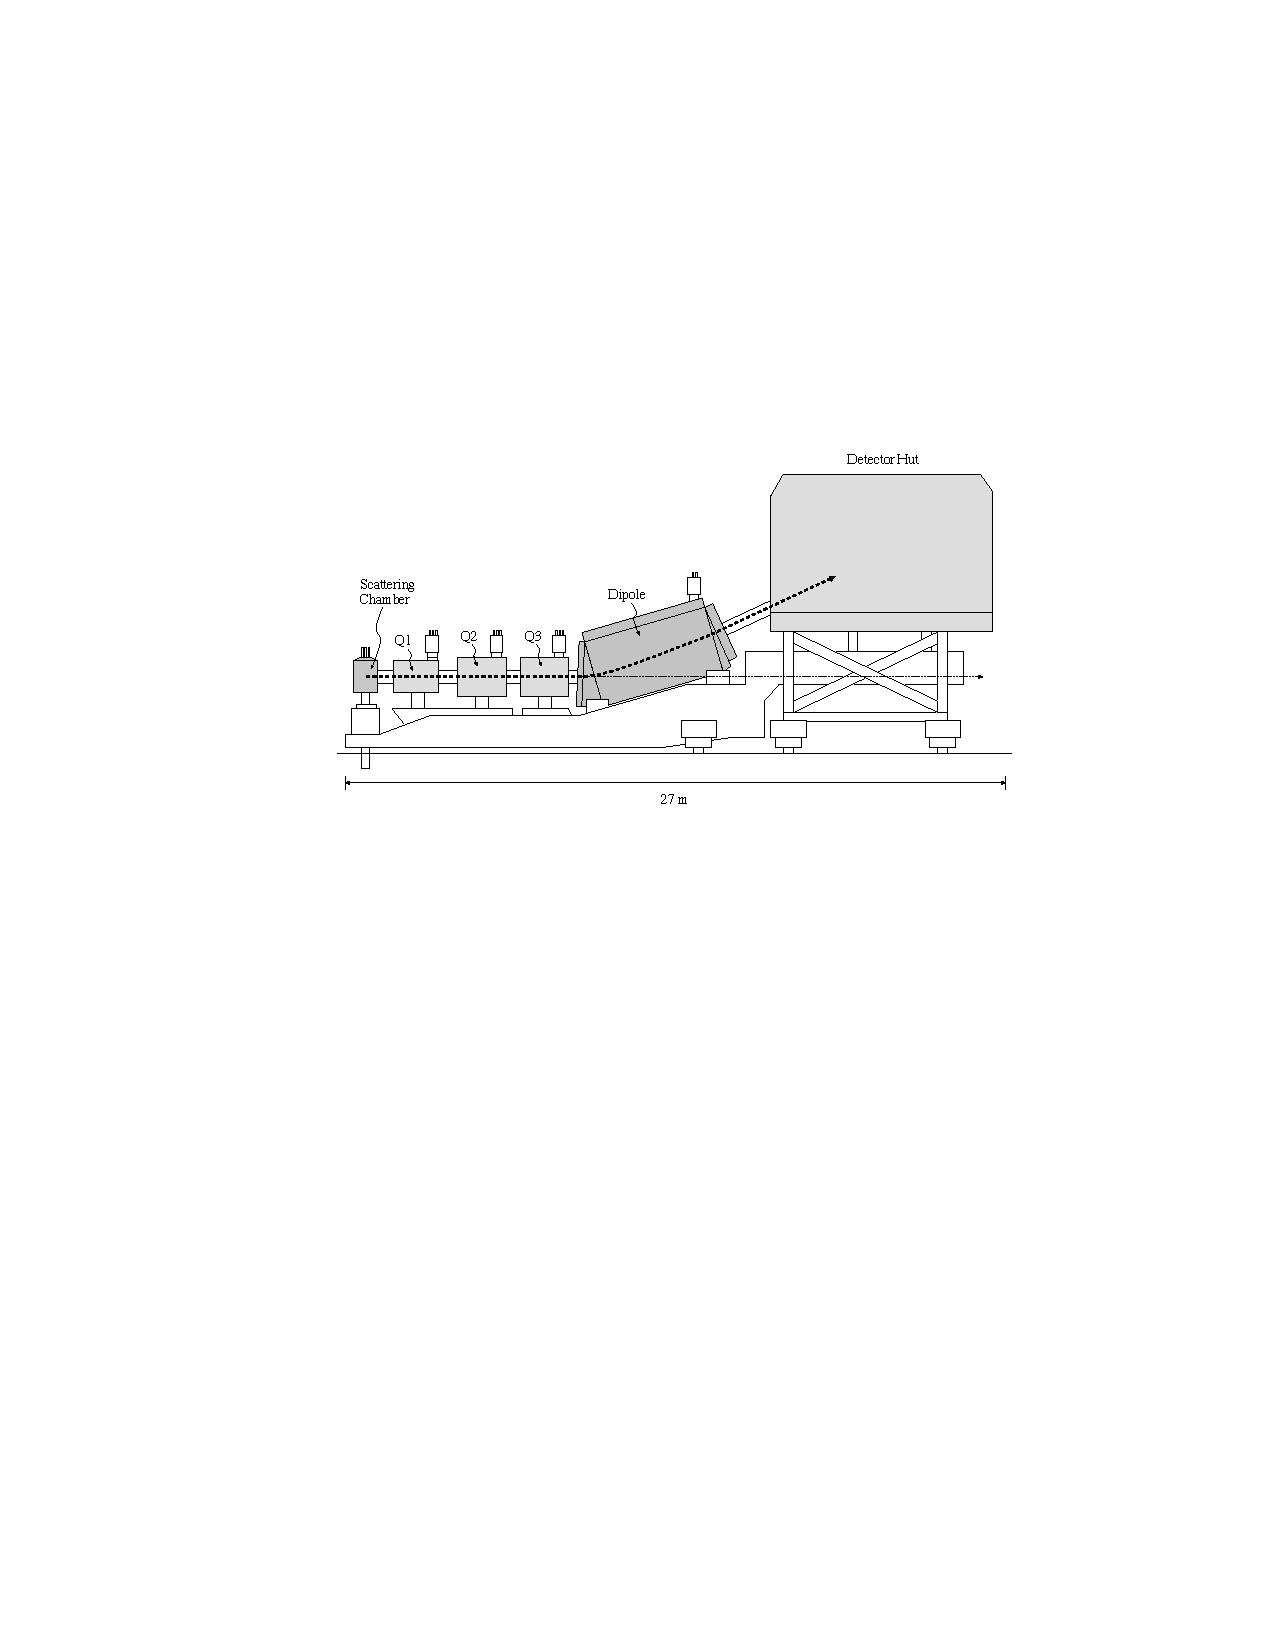
\includegraphics[width=1.0\textwidth]{chap3/hms_schematic.pdf}
    \caption{High Momentum Spectrometer (HMS) side view.}
    \label{fig:hms_schematic}
\end{figure}

The HMS's performance is well understood from 6 GeV era experiments, but
some changes have been made for the 12 GeV era.
The dipole NMR probe was moved outside the dipole for more accurate measurement
of central momenta.
The original HMS drift chambers were replaced with a pair of drift chambers
that match the design of those in the SHMS.

Optics calibration runs\footnote{HMS singles with run numbers 1337–1352}
using hydrogen elastic scattering and carbon data were taken to determine
central dipole field values, external NMR measurements, and corresponding
magnet currents.
These data were also used to characterize spectrometer mispointing and angular
offsets and optimize the matrix used in projecting tracks from the focal
plane to the interaction at the target.
See \cite{Holly_HMS_Optics} for more details.

\subsection{Super High Momentum Spectrometer}
Like the HMS, the SHMS is an 18.4$^{\circ}$ vertical bend spectrometer with
superconducting magnets in a QQQD configuration.
To allow it to reach smaller scattering angles, the SHMS has an additional
3$^{\circ}$ horizontal bender (HB) dipole before the first quadrupole.
Its maximum central momentum is 11 GeV with an acceptance covering $-10\%$
to $+22\%$.
The SHMS detector stack consisting of a hodoscope, lead glass calorimeter,
three Cherenkov counters, and pair of drift chambers sits in a concrete
shielding hut approximately 22 m from the target chamber.

\begin{figure}[!h]
    \centering
    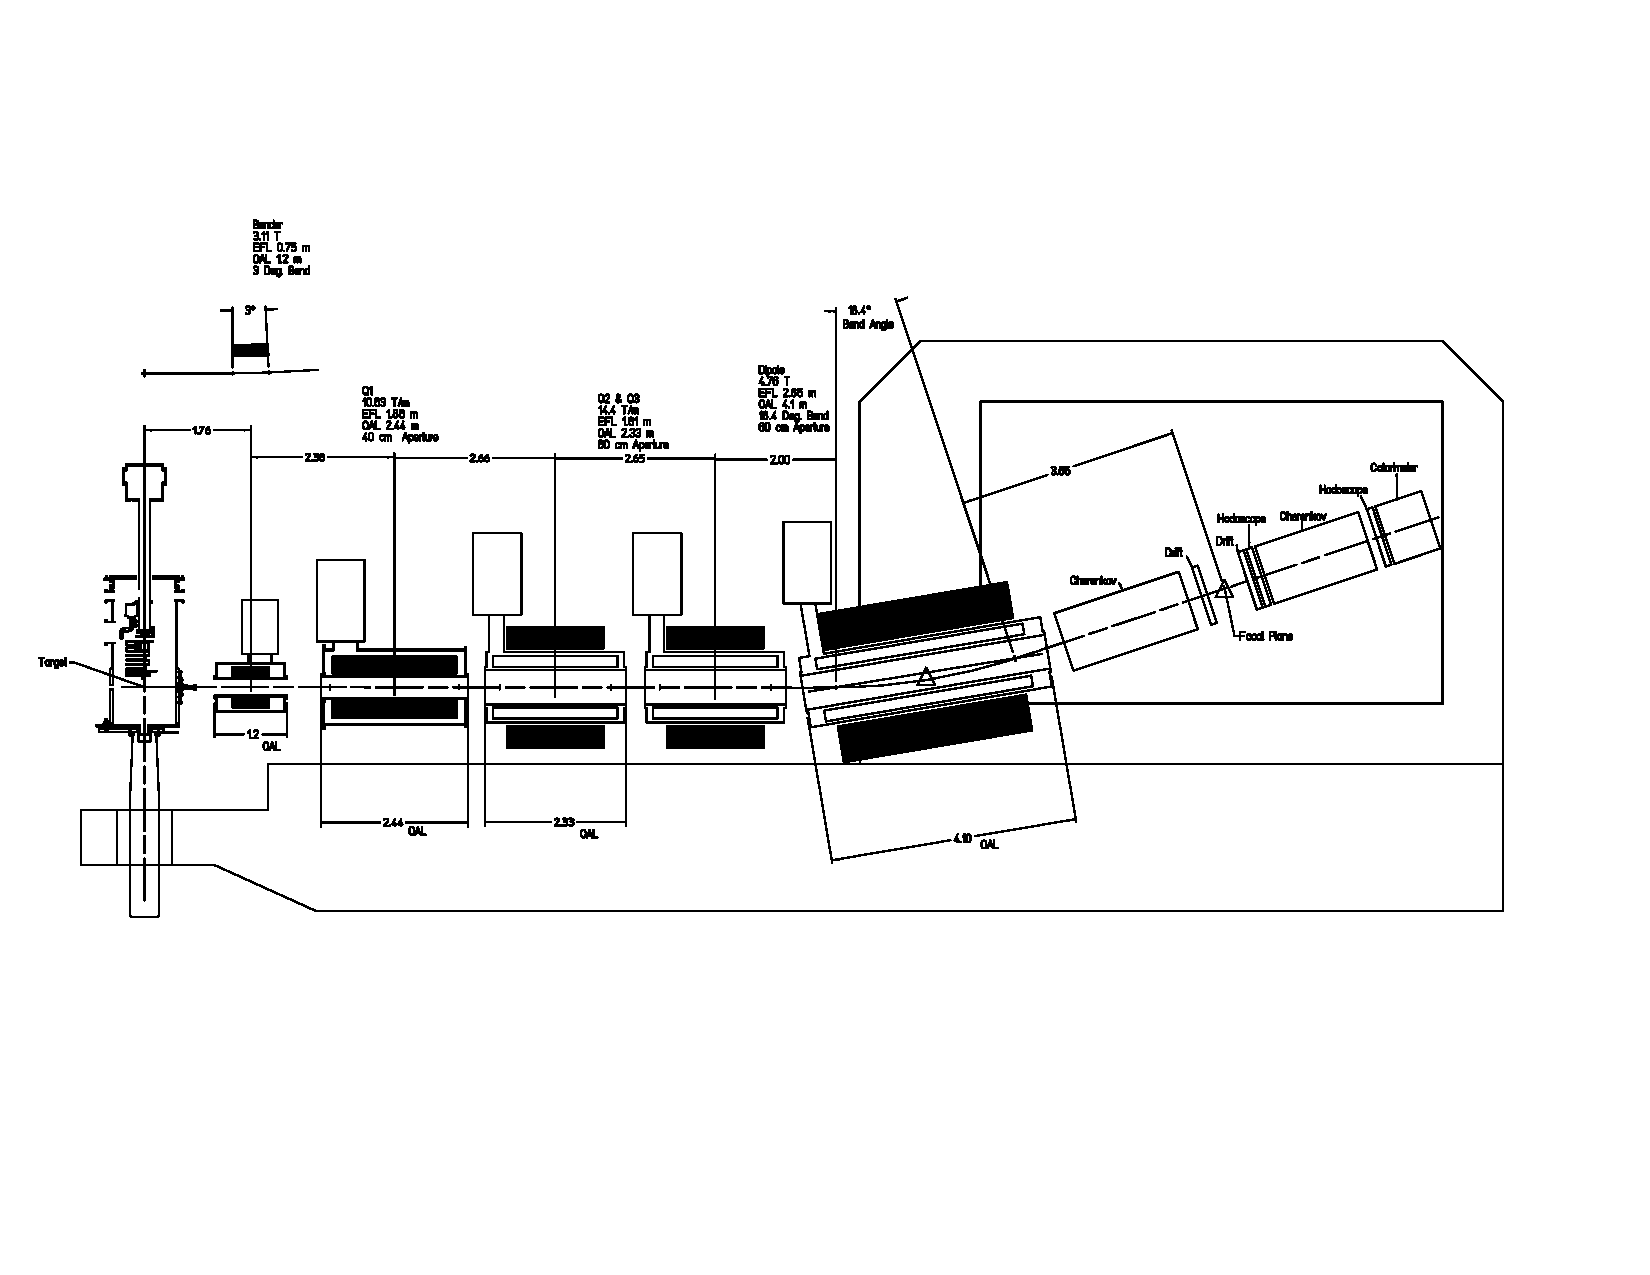
\includegraphics[width=1.0\textwidth]{chap3/SHMS_Layout_new.pdf}
    \caption{Super High Momentum Spectrometer (SHMS) side view.}
    \label{fig:hms_schematic}
\end{figure}

As with the HMS, she commissioning of the SHMS magnets used hydrogen and carbon
elastic scattering and the 4.4 MeV carbon excited peak to characterize
spectrometer mispointing and angular offsets and optimize the track
reconstruction matrix.
See \cite{Holly_SHMS_Optics} for more details.

\subsection{Collimators and Slit Systems}
The HMS has a remotely operated collimator ladder installed on the front face
of Q1.
The HMS ladder contains one sieve-slit for optics tuning and two
solid-angle-defining collimators.

The SHMS has a similar system installed on the front face of Q1.
The SHMS ladder contains two sieve-slits for optics tuning and one
solid-angle-defining collimator.
The two sieve slits consist of a lattice of holes separated by 0.6457"
horizontally and 0.9843" vertically.
Two holes in each sieve are missing to ensure correct orientation.
To account for the HB magnet, the SHMS has an additional sieve slit ladder
placed immediately upstream from the HB.

\section{Detector Packages}
The detector stacks in both spectrometers consist of a lead glass calorimeter,
one or more Cherenkov counters, a hodoscope, and a pair of drift chambers.
Details beyond what are covered here can be found
online~\cite{Standard_Equipment_Manual}.

\subsection{Hodoscopes}

The HMS and SHMS hodoscopes consist of two pairs of X/Y planes
that generate the basic trigger for the DAQ system and provide an initial
estimate of particle velocity based on time of flight (TOF).
Each X (Y) plane consists of some number of horizontally (vertically) oriented
paddles.
All paddles except those in the SHMS S2Y are plastic scintillators.
The HMS paddles are BC-404~\cite{Standard_Equipment_Manual,BC404}.
The SHMS S1X, S1Y, and S2X paddles are RP-408~\cite{SHMS_hodo_plastic,RP408}.
The SHMS S2Y paddles are quartz~\cite{SHMS_hodo_quartz}.
In both spectrometers the first pair of planes, S1X and S1Y, are
about \SI{2.2}{m} upstream from the second pair of planes, S2X and S2Y.
Table~\ref{tab:hodoscope_characteristics} contains a summary of each plane.

\begin{figure}[!h]
    \centering
    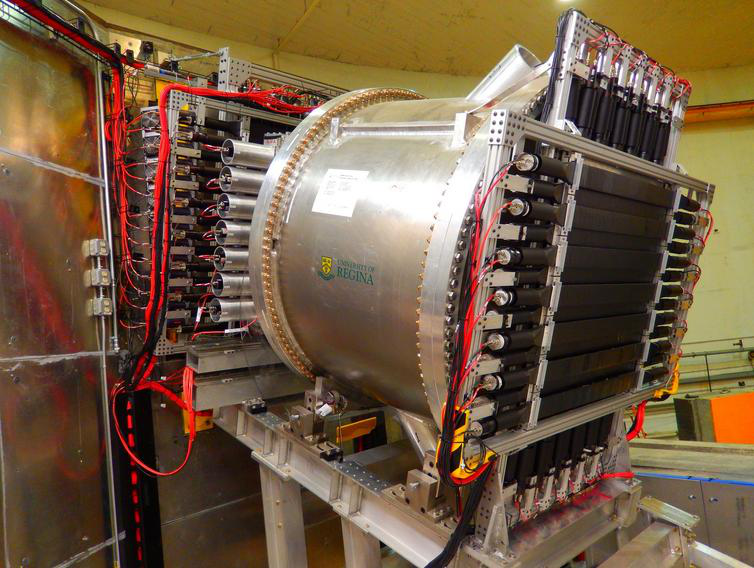
\includegraphics[width=1.0\textwidth]{chap3/shms_hodoscope.png}
    \caption{The two pairs of hodoscope planes that make up the SHMS
             hodoscope are placed on either side of Aerogel and Heavy Gas
             Cherenkov detectors.}
    \label{fig:shms_hodoscope}
\end{figure}

\begin{table}[h]
    \centering
    \caption{Summary of the HMS and SHMS hodoscopes}
    \label{tab:hodoscope_characteristics}
    \resizebox{1.0\textwidth}{!}{
        \begin{tabular}[t]{lcccccccc}
            \hline
            \hline
            Parameter                            & \multicolumn{4}{c}{HMS} & \multicolumn{4}{c}{SHMS} \\
                                                 & S1X & S1Y & S2X & S2Y & S1X & S1Y & S2X & S2Y \\
            \hline

            Width (mm)                           & 8.0 & 8.0 & 8.0 & 8.0 & 8.0 & 8.0 & 10.0 & 5.5 \\
            Thickness (mm)                       & 1.0 & 1.0 & 1.0 & 1.0 & 5.0 & 5.0 & 5.0 & 2.5 \\
            Length (mm)                          & 75.5 & 120.5 & 75.5 & 120.5 & 100.0 & 100.0 & 110.0 & 125 \\
                                                     \\
            z-position (cm)                      & 77.83 & 97.52 & 298.82 & 318.51 & 52.1 & 61.7 & 271.4 & 282.4 \\
            Pitch (cm)                           & 7.5  & 7.5  & 7.5  & 7.5  & 7.5  & 7.5  & 9.5  & 5.0  \\
            $\delta$z from odd numbered          & 2.12 & 2.12 & 2.12 & 2.12 & 2.12 & -2.12 & -2.12 & -5.4 \\
            to even numbered paddles             &   &   &   &   &   &   &   &   \\
                                                     \\
            Paddles per plane                    & 16 & 10 & 16 & 10 & 13 & 13 & 14 & 21 \\
                                                     \\
            Material                             & BC404 & BC404 & BC404 & BC404 & RP408 & RP408 & RP408 & Quartz \\
            \hline
        \end{tabular}
    } % resizebox
\end{table}

Plastic scintillators are solid plastics that contain organic scintillating
compounds: aromatic hydrocarbons containing linked or condensed benzene-ring
structures~\cite{Leo_1994}.
Light produced in plastic scintillators is generated by transitions of free
valence electrons belonging to $\pi$-molecular orbitals.
When a particle passes through the material, it excites electrons to either a
singlet or triplet state, as well as a vibrational mode of the molecule,
as shown in figure~\ref{fig:leo_scintillator_energy_levels}.

\begin{figure}[!h]
    \centering
    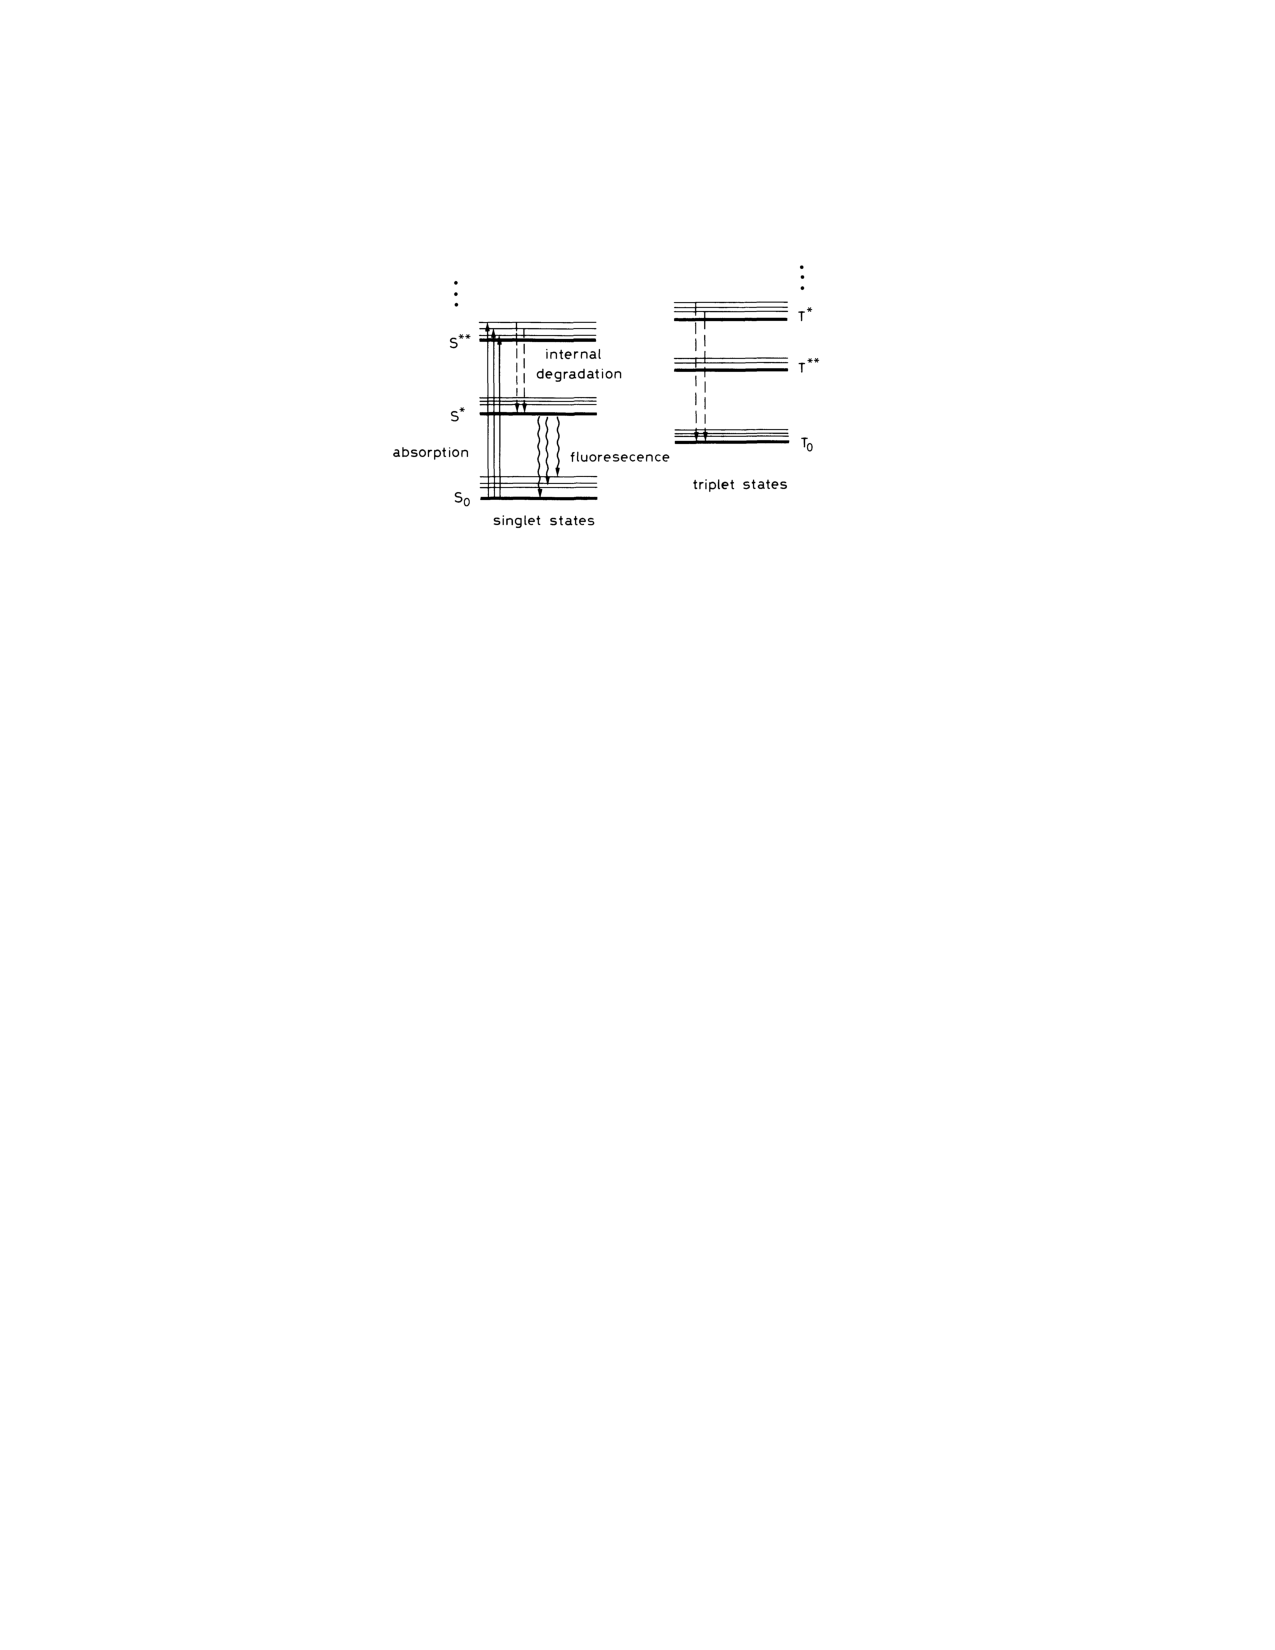
\includegraphics[width=0.6\textwidth]{chap3/leo_scintillator_energy_levels.pdf}
    \caption{A schematic diagram of the energy levels of an organic
             scintillator~\cite{Leo_1994}. Particles passing through the
             material will excite valence electrons to singlet and triplet
             states, decay from which will create visible light.}
    \label{fig:leo_scintillator_energy_levels}
\end{figure}

An electron excited to the $S^{**}$ state will quickly decay to $S^*$ without
radiation, and then radiatively decay to a vibrational state of the ground
state $S_0$ within a few nanoseconds.
The energy of the radiation is less than that required to excite an electron
from $S_0$ to $S^*$, so none of it will be absorbed in the process.
The material is transparent to its own radiation.

The transition from a triplet state is similar.
Decay from $T_0$ to $S_0$ is possible, but suppressed by selection rules.
The decay typically takes place when two $T_0$ molecules interact with each
other, resulting in one in the excited $S^*$ state, one in the ground state,
and heat dissipated in the medium. The excited $S^*$ molecule then radiatively
decays as in the singlet case.

Light produced in the SHMS quartz plane is Cherenkov radiation, which is
discussed further in the subsection on Threshold Cherenkov Counters.
% No neutrons produce C rad, so can use S2Y as a veto

Both ends of each HMS paddle are read out by Philips XP2282B PMTs, with
nominal operating voltages of $\sim\SI{1800}{V}$~\cite{HMS_hodoscope_HV}.
Similarly, the ends of each SHMS paddle are read out by a combination of ET
ET9214B, ET ET9814QB, Photonis XP2262B, and Photonis XP2020QB PMTs.
The operating voltages for each SHMS hodoscope PMT are available on the Hall C
Wiki~\cite{SHMS_hodoscope_plastic_HV, SHMS_hodoscope_quartz_HV}.

The signals from each PMT are fed into a passive splitter, yielding two signals
with amplitudes 1/3 and 2/3 of the original.
The smaller signal is sent to a flash Analog-to-Digital Converter (fADC).
The larger is sent to a discriminator as part the core of the trigger system,
which will be discussed in the next section.

\subsection{Drift Chambers}
\label{subsec:drift_chambers}
Both spectrometers have a pair of drift chambers~\cite{SHMS_drift_chambers}
that provide precise tracking information.
Combined with knowledge of the spectrometers' optics, this tracking information
is used to calculate particle momenta, angles, and positions at the interaction
point in the target.

\begin{figure}[!h]
    \centering
    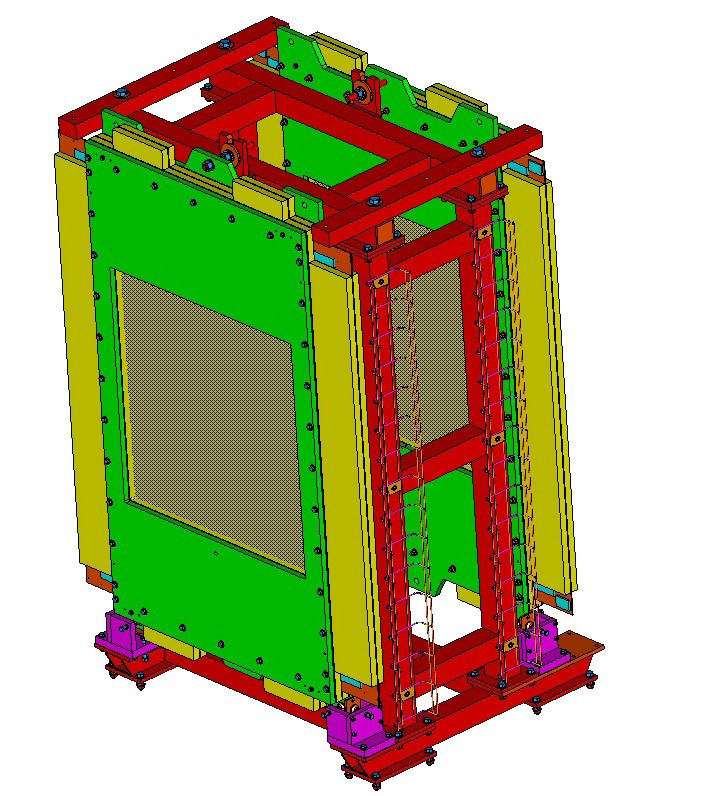
\includegraphics[width=0.6\textwidth]{chap3/shms_dc.png}
    \caption{A rendering  of the SHMS drift chambers mounted in the detector
             hut frame.}
    \label{fig:shms_dc}
\end{figure}

The drift chamber packages consist of a pair of identical chambers, each of
consists of six wire planes.
Each chamber has an active area of 80x80\si{\cm\squared} to match the size of
the SHMS's acceptance and focal plane.
Copper-coated mylar cathode planes are placed between each wire plane, before
the first plane, and after the last plane.
Each wire plane consists of a set of alternating \SI{20}{\micro\meter} gold
tungsten sense (anode) wires and \SI{80}{\micro\meter} field wires, separated
by \SI{500}{\micro\meter}.
To reduce cost, only two wire orientations were manufactured: an X plane with
horizontally oriented wires and a U plane with wires oriented 60$^{\circ}$ from
the X wires, both of which are shown in figure~\ref{fig:dc_planes}.
In the SHMS, the U planes have 109 sense wires per plane and the X planes have
79.
In the HMS, the U planes have 96 sense wires per plane and the X planes have
102.

\begin{figure}[h]
    \centering
    \begin{subfigure}[b]{0.4\textwidth}
        \centering
        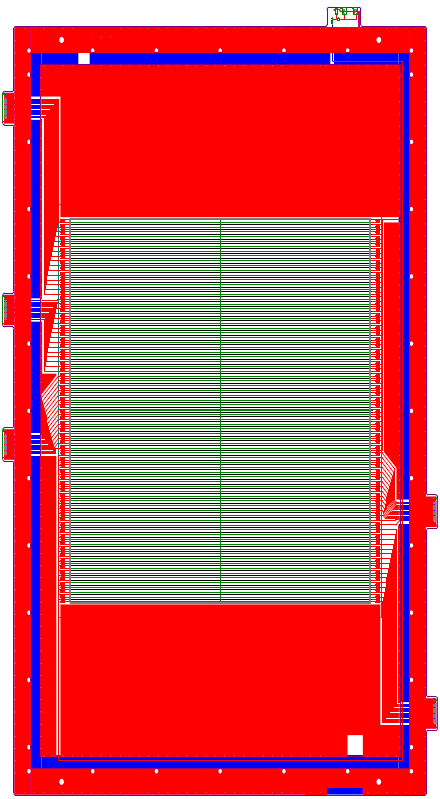
\includegraphics[width=\textwidth]{chap3/shms_dc_x_plane.png}
        \caption{X plane}
        \label{fig:dc_x_plane}
    \end{subfigure}
    \hfill
    \begin{subfigure}[b]{0.4\textwidth}
        \centering
        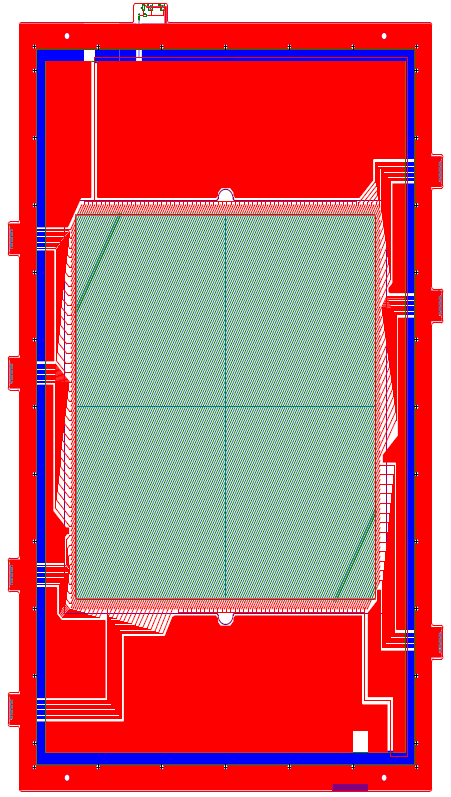
\includegraphics[width=\textwidth]{chap3/shms_dc_u_plane.png}
        \caption{U plane}
        \label{fig:dc_u_plane}
    \end{subfigure}
    \caption{The drift chambers consist of 6 wire planes with different
             orientations, each of which are generated by rotating the two
             X and U planes.}
    \label{fig:dc_planes}
\end{figure}

X' and U' planes, with identical wire orientations offset by
\SI{500}{\micro\meter} from the unprimed planes, can be generated by rotating
an X or U plane 180$^\circ$ such that the top becomes the bottom.
V and V' planes, with wires oriented -60$^\circ$ from the X wires, can be
generated by rotating the U and U' planes 180$^\circ$ around a vertical axis
running through the center of the plane.
The offset between the primed and unprimed planes allows us to resolve the
left-right ambiguity of each hit\footnote{For a hit on an isolated drift
chamber wire, it is impossible to know whether the ionized electrons came from
the right or the left of the wire. This will be discussed further in the
chapter on data analysis.}

\begin{figure}[!h]
    \centering
    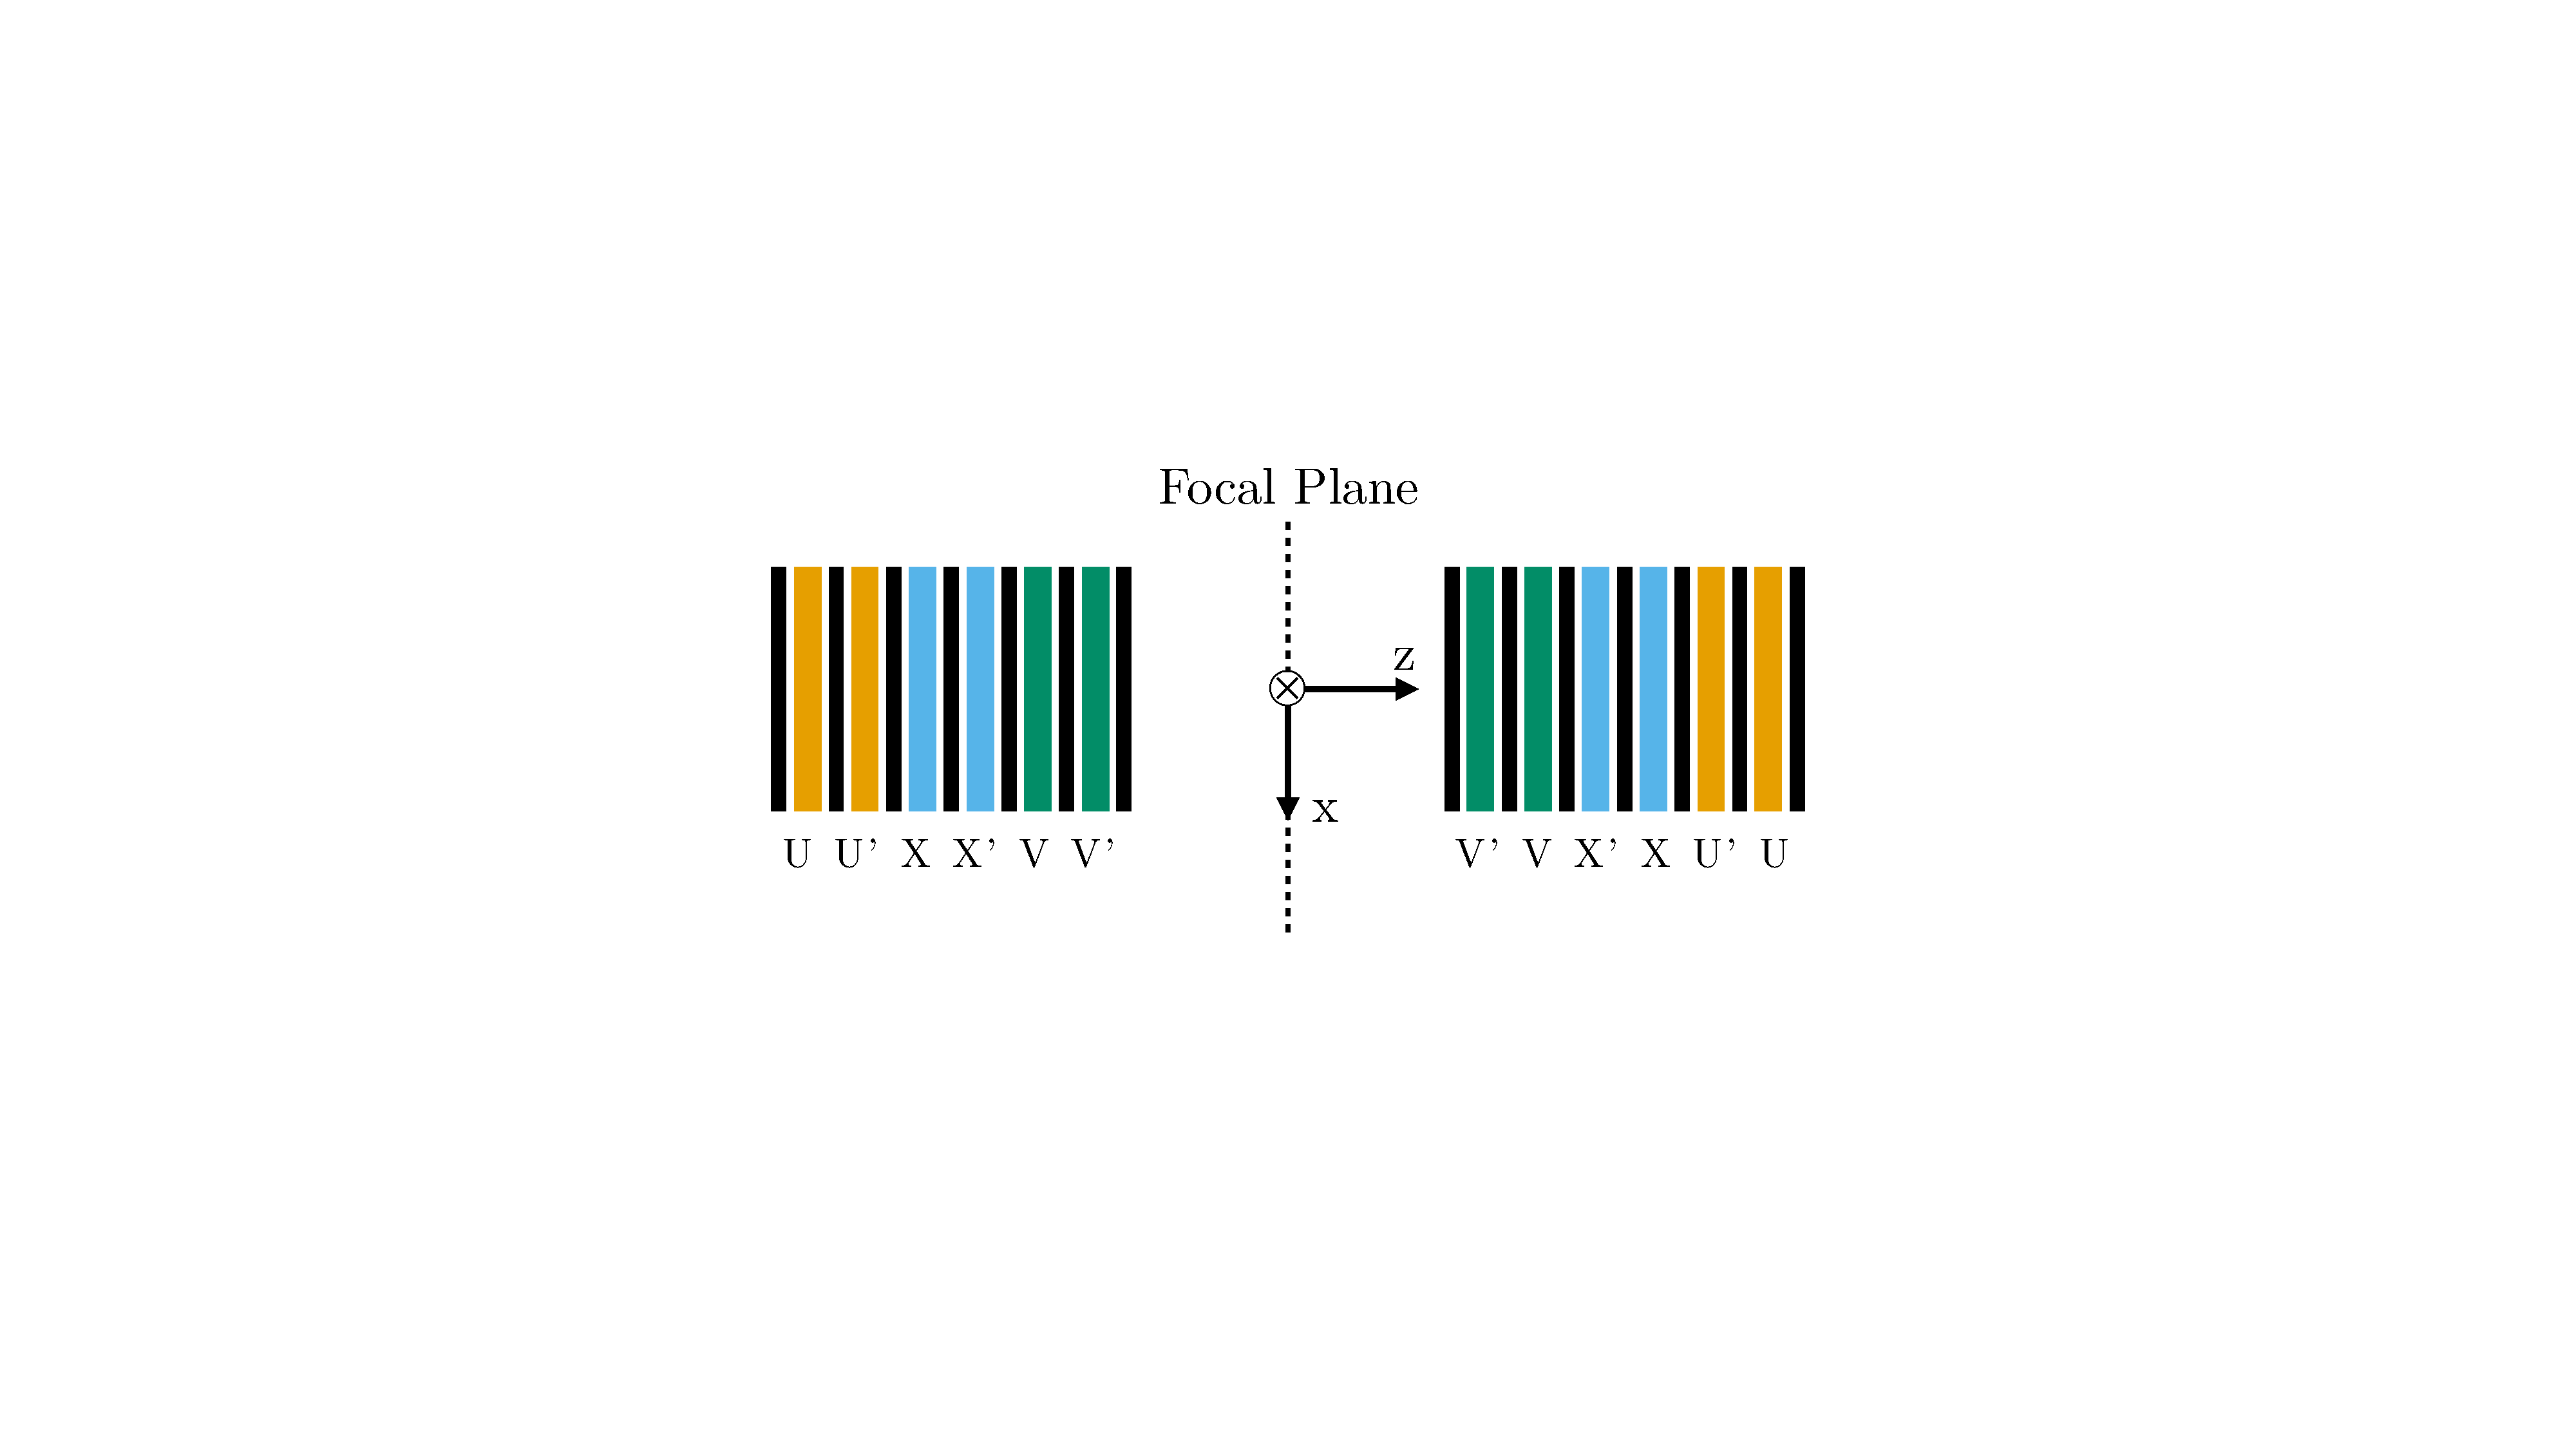
\includegraphics[width=0.6\textwidth]{chap3/dc_plane_order.pdf}
    \caption{Side view of the order of planes encountered by a particle
             traveling through the SHMS. The focal plane of the spectrometer
             is roughly halfway between the two drift chambers.}
    \label{fig:shms_plane_order}
\end{figure}

As shown in figure~\ref{fig:shms_plane_order}, the order of the planes in the
first chamber encountered by a particle traveling through the SHMS is
(U,U',X,X',V,V').
The order in the second chamber is reversed.
In the HMS, the V and V' planes in each chamber are swapped.

During operation, each chamber is filled with a 50/50 mix of argon and ethane.
When a charged particle passes through the chamber, it will ionize some of
the gas.
The cathode planes and field wires are kept at $\sim-\SI{1900}{V}$ with respect
to the sense wires kept at ground, creating an electric field pointing from
sense wires toward field wires and cathode planes.
The field accelerates these primary ionized electrons toward the sense wires,
ionizing more electrons along the way.
The resulting cloud of electrons drifts toward sense wires at a
constant ``drift velocity.''

The electrons are collected by sense wires which are read out by
16-channel discriminators attached to the chamber supports.
The discriminators are fed, via 16-channel ribbon cables, to CAEN 1190
TDCs~\cite{CAEN_1190_manual} in a VXS crate in the detector huts.
When the 1190s receive a pretrigger, they record the time of the last several
hits\footnote{The trigger and readout electronics will be discussed in more
detail in the next section.}.
The time between the pretrigger and the time at which the electron cloud hits
a wire can be used to determine the distance at which the initial ionization
occurred.
Using this information from every wire plane in both chambers allows
precise track reconstruction with residuals of \SI{250}{\micro\meter} in the
SHMS and (\SI{350}{\micro\meter} in the HMS.
The complete process of converting raw signals from each wire to full tracking
information will be discussed in section~\ref{sec:daq}.

\subsection{Threshold Cherenkov Counters}
Threshold Cherenkov counters make use of a particle-dependent Cherenkov
radiation threshold to discriminate between types of particles.
A charged particle with mass $m$, velocity $\beta$, and 3-momentum $p$ passing
through a medium with index of refraction $n$ will emit Cherenkov radiation if
\begin{equation}
    \frac{c}{n} < \beta = \frac{p}{\sqrt{p^2+m^2}}
\end{equation}
or equivalently, as illustrated in figure~\ref{fig:hms_cer_threshold},
\begin{equation}
    1-\frac{c}{n} > 1-\beta = 1-\frac{p}{\sqrt{p^2+m^2}}
\end{equation}

% HMS has C4F8O at 0.45 atm.  % n=1.00137 @ 1 atm per https://userweb.jlab.org/~hcf/shmsnim/shmsNIM.pdf
\begin{figure}[!h]
    \centering
    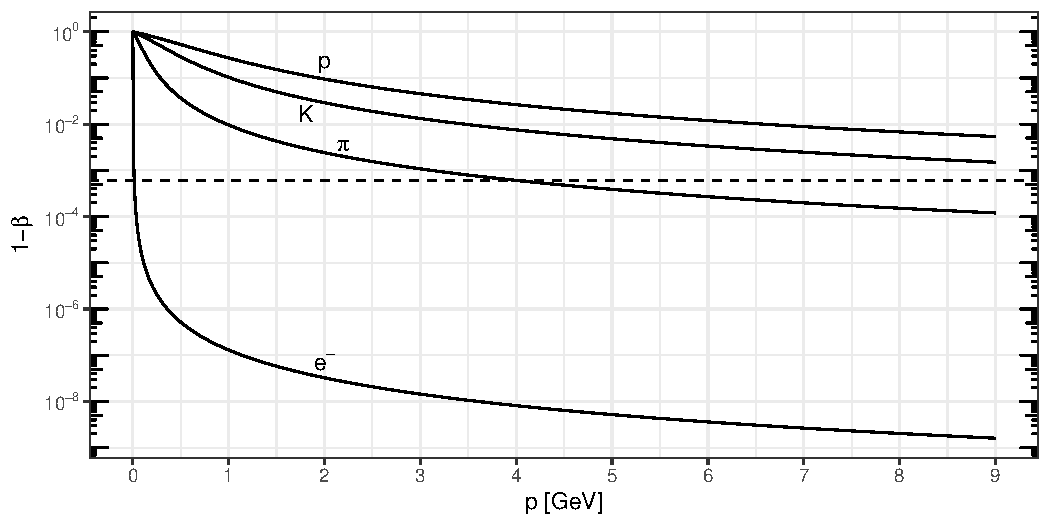
\includegraphics[width=1.0\textwidth]{chap3/hms_cer_threshold.pdf}
    \caption{Value of $1-\beta$ for various particles as a function of
            momentum. The horizontal line represents the Cherenkov threshold
            for \ch{C4F8O} at a pressure of 0.45 atm, below which a particle
            will produce Cherenkov radiation.
            }
    \label{fig:hms_cer_threshold}
\end{figure}

Over a sufficiently narrow range of momenta, only some types of particles will
emit Cherenkov radiation.
For example, for a threshold Chereknov counter filled with \ch{C4F8O} at
0.45 atm, the presence or absence of Cherenkov radiation can be used to
determine if the particle that generated a trigger is an electron or a hadron,
provided the momentum range in question is below $\sim$4 \si{\giga\eV}.
Given knowledge of the expected range of momenta an experiment requires and
what types of backgrounds will need to be removed, one can pick an appropriate
Cherenkov medium based on its index of refraction. Further tuning of the
threshold can be done by adjusting the pressure of the gas, making use of
the fact that pressure is proportional to $n-1$.

% TODO: make ggplot label gases' thresholds
\begin{figure}[!h]
    \centering
    \includegraphics[width=1.0\textwidth]{chap3/cer_gas_thresholds.pdf}
    \caption{Value of $1-\beta$ for various particles as a function of
            momentum. The horizontal lines represent the Cherenkov threshold
            for various gases at 1 atm, below which a particle
            will produce Cherenkov radiation.
            % TODO: add gass and particle labels to figure
            }
    \label{fig:cer_gas_threshold}
\end{figure}

Suppose a threshold Cherenkov detector has
light-gathering efficiency $\epsilon_c(\lambda)$,
a PMT with quantum efficiency $QE(\lambda)$,
and is filled with a gas with transparency $G(\lambda)$
and index of refraction $n$.
It can be shown~\cite{NGC_Design_Report} that by a particle of charge $e$ passing through the detector
with velocity $\beta$ and path length $L$ will generate
$N_e =AL\left(1-\frac{1}{\beta^2n^2}\right)$ photoelectrons, where
\begin{equation}
A = 2 \pi \alpha \int_{\lambda_1}^{\lambda_2} \epsilon_c(\lambda)QE(\lambda)G(\lambda)\frac{d\lambda}{\lambda^2}.
\end{equation}

The gas Cherenkov detectors in the HMS and SHMS use spherical mirrors to focus
Cherenkov radiation onto PMTs mounted on the back of the detector. The SHMS
aerogel Cherenkov consists of an aerogel tray, covered in either GORE or
Millipore diffusion materials~\cite{Horn_2017}, mounted between two columns
of PMTs.

\subsubsection{HMS Cherenkov}
% Some leads for hunting down the original article. Could just ask Donal
% https://www.osti.gov/biblio/374934
% http://flux.aps.org/meetings/YR9596/BAPSAPR95/abs/SJ0805.html
% https://uva.worldcat.org/title/a-threshold-gas-cerenkov-detector-for-cebafs-hall-c-high-momentum-spectrometer/oclc/4436255400?referer=brief_results

\begin{figure}[ht]
    \centering
    \begin{subfigure}[b]{0.4\textwidth}
        \centering
        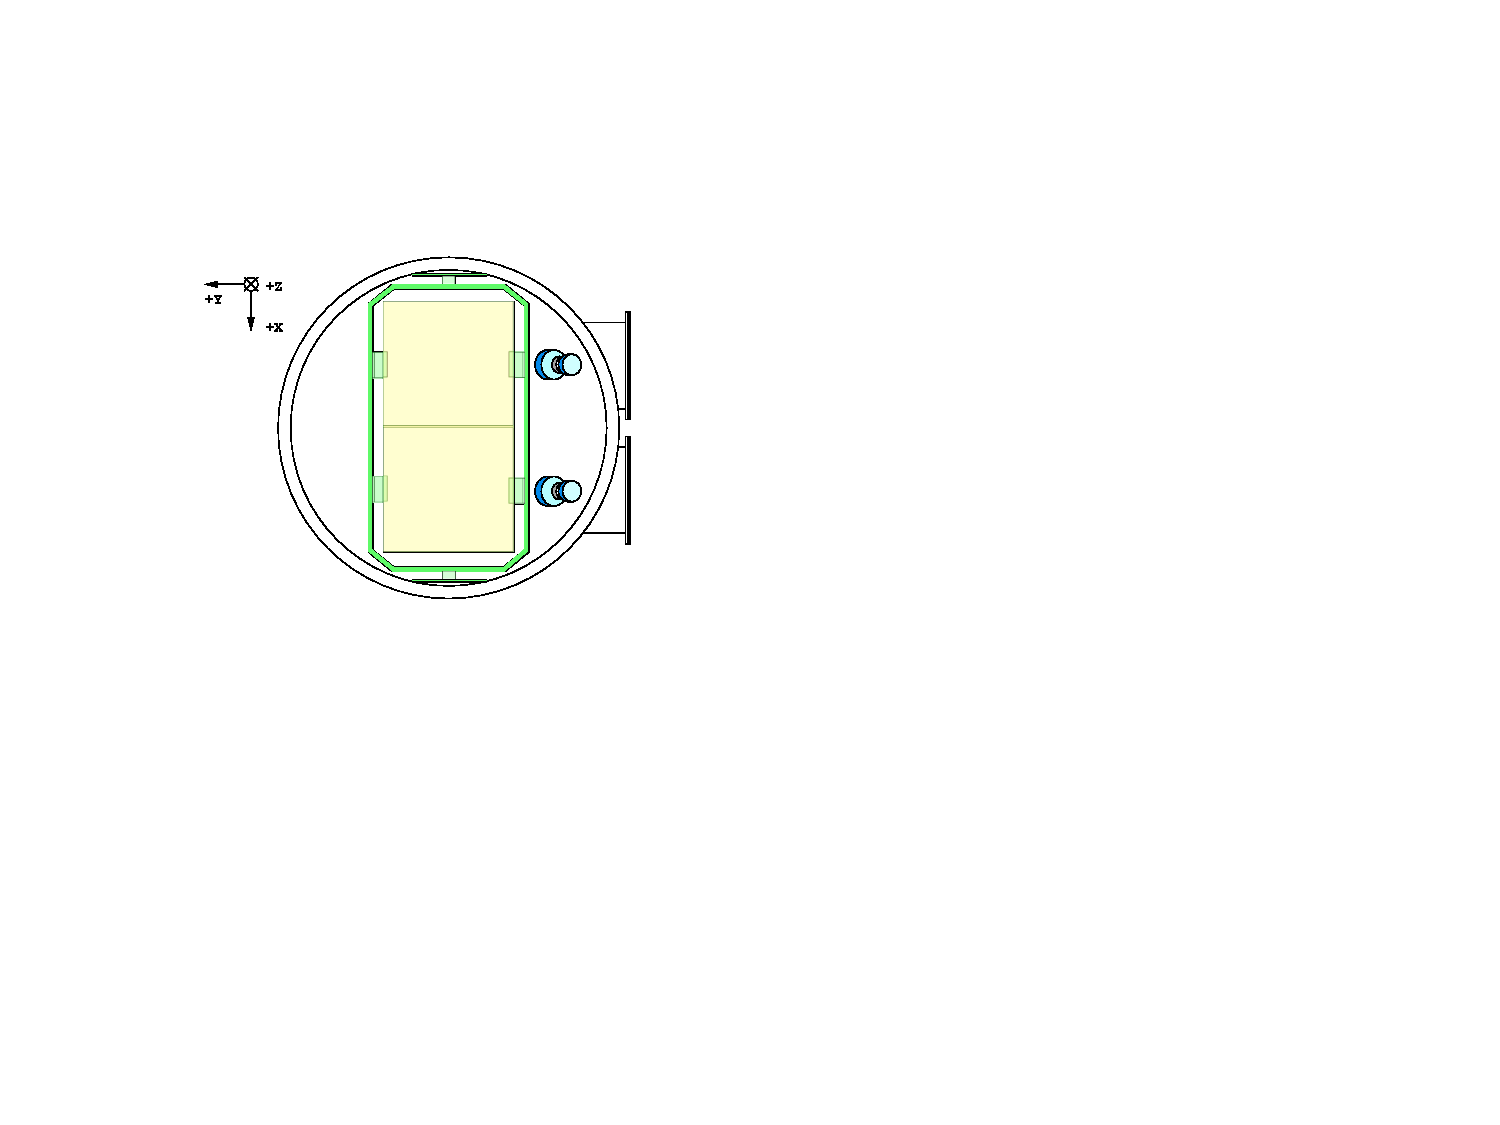
\includegraphics[width=\textwidth]{chap3/hms_cer_front.pdf}
        \caption{Front view}
        \label{fig:hms_cer_front}
    \end{subfigure}
    \hfill
    \begin{subfigure}[b]{0.4\textwidth}
        \centering
        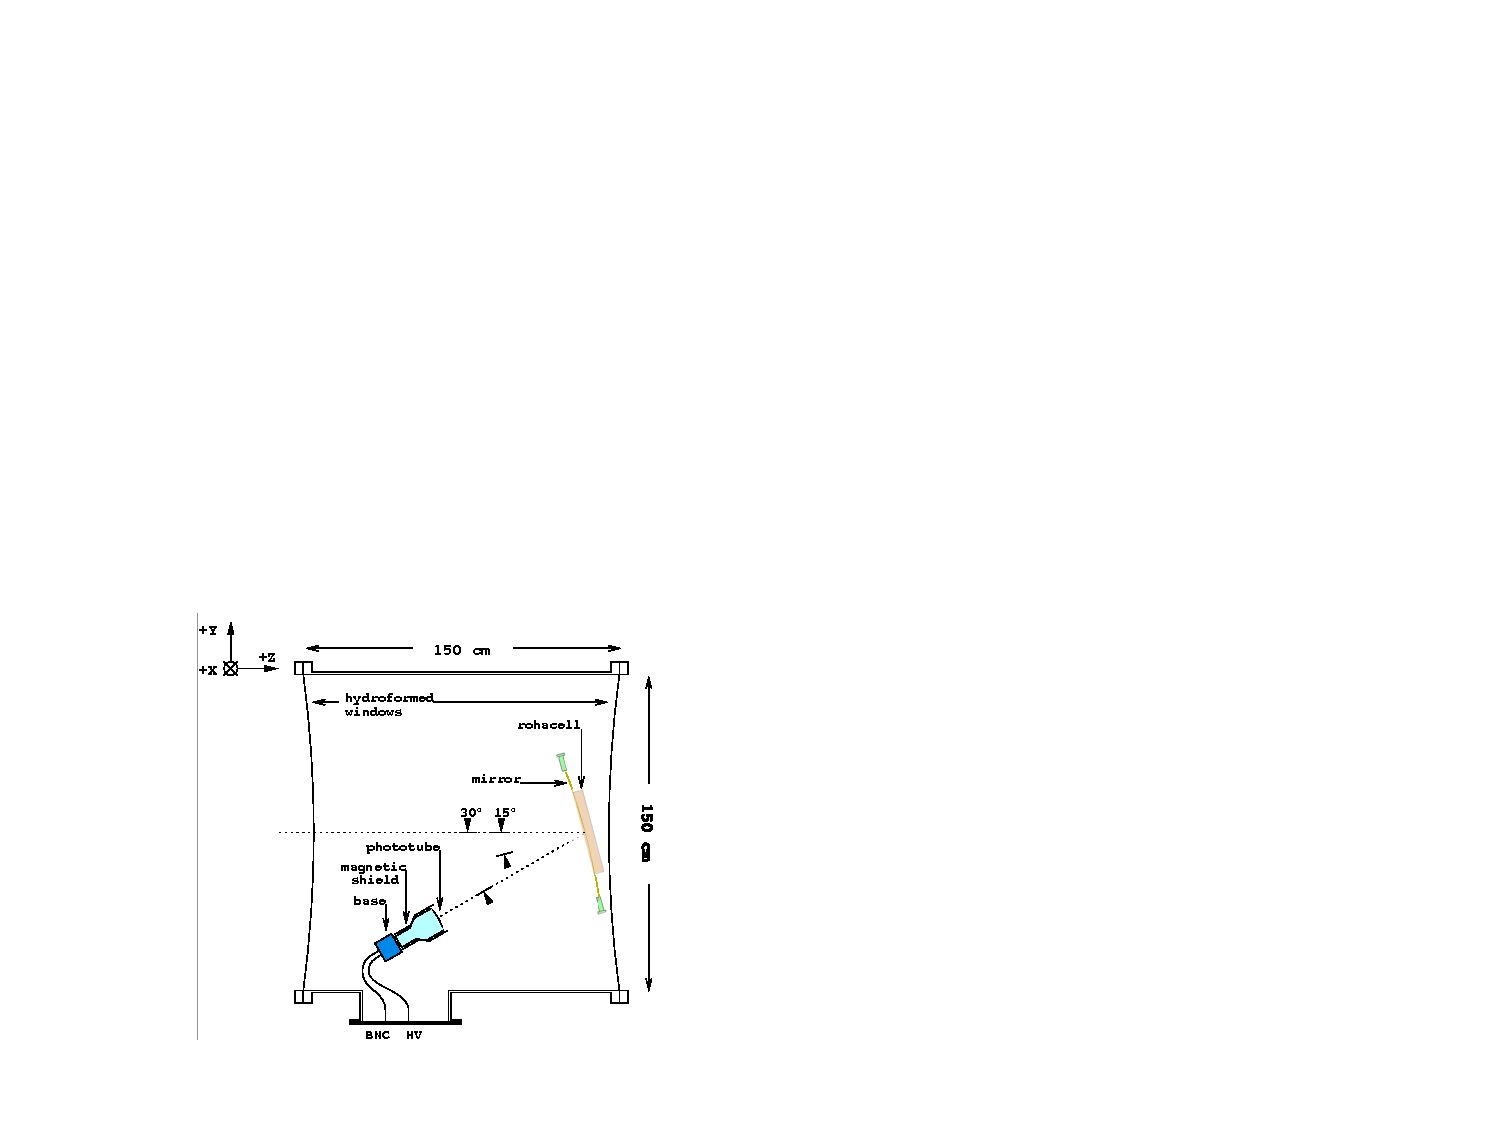
\includegraphics[width=\textwidth]{chap3/hms_cer_top.pdf}
        \caption{Top view}
        \label{fig:hms_cer_top}
    \end{subfigure}
    \caption{The HMS Cherenkov}
    \label{fig:hms_cherenkov}
\end{figure}

The HMS Cherenkov~\cite{Cothran_1995} is designed for electron-pion separation.

During our runs, it was filled with \ch{C4F8O} at 0.45 atm.

Broken mirror during our runs. Will discuss diagnosis in later section.

\subsubsection{SHMS Noble Gas Cherenkov}
\begin{figure}[ht]
    \centering
    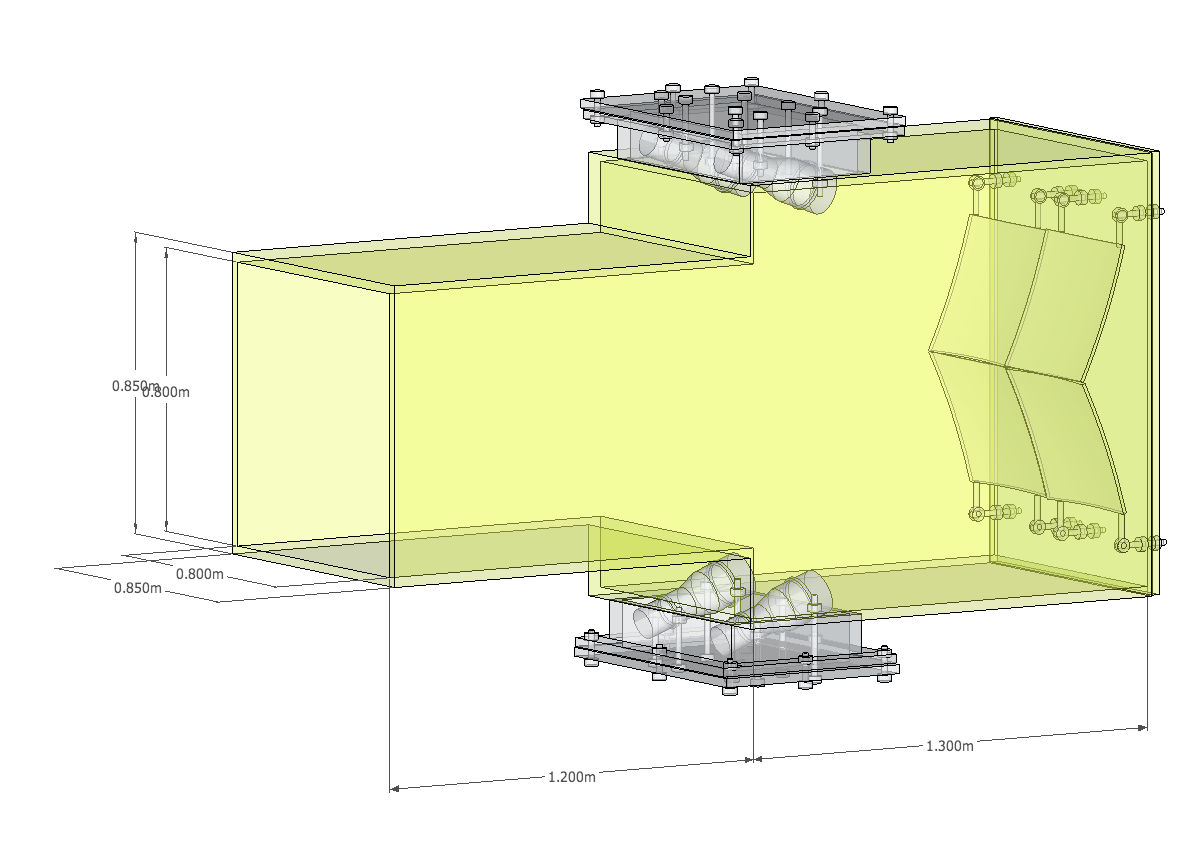
\includegraphics[width=1.0\textwidth]{chap3/shms_ngc_render.png}
    \caption{The SHMS Noble Gas Chereknov }
    \label{fig:shms_ngcer}
\end{figure}

% CO2 at 1 atm.
The SHMS Noble Gas Cherenkov~\cite{NGC_Design_Report} is designed for e/pi
separation.

During our runs, it was filled with \ch{CO2} at 1 atm.

\subsubsection{SHMS Heavy Gas Cherenkov}
\begin{figure}[ht]
    \centering
    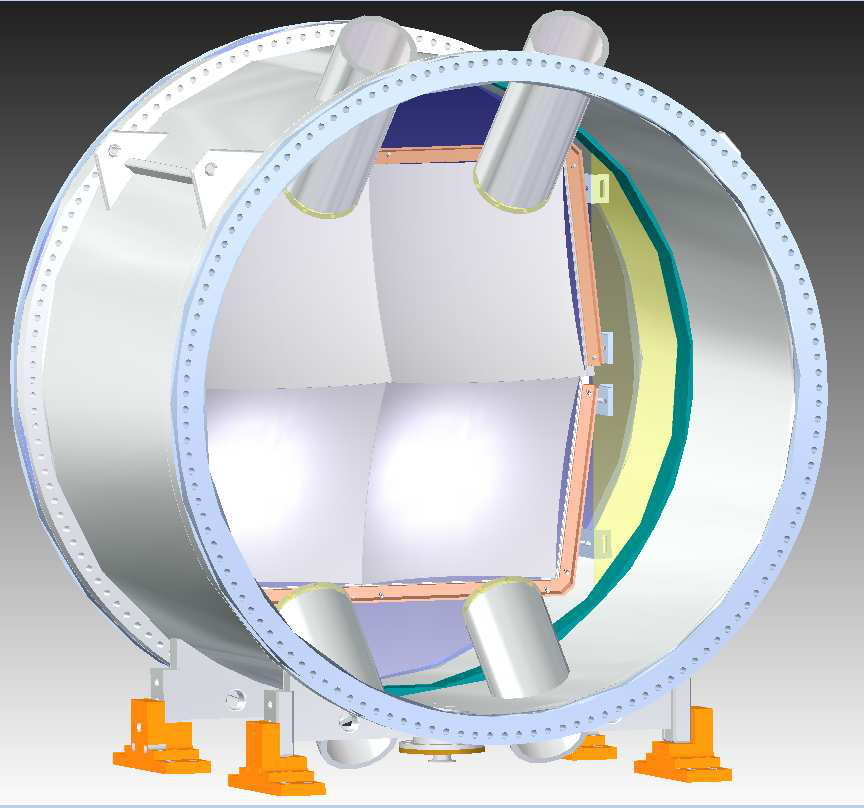
\includegraphics[width=0.5\textwidth]{chap3/shms_hgc_render.png}
    \caption{The SHMS Heavy Gas Chereknov }
    \label{fig:shms_hgcer}
\end{figure}

% CO2 at 1 atm.
Designed for pi/K separation.

During our runs, it was filled with \ch{CO2} at 1 atm.

\subsubsection{SHMS Aerogel Cherenkov}
\begin{figure}[ht]
    \centering
    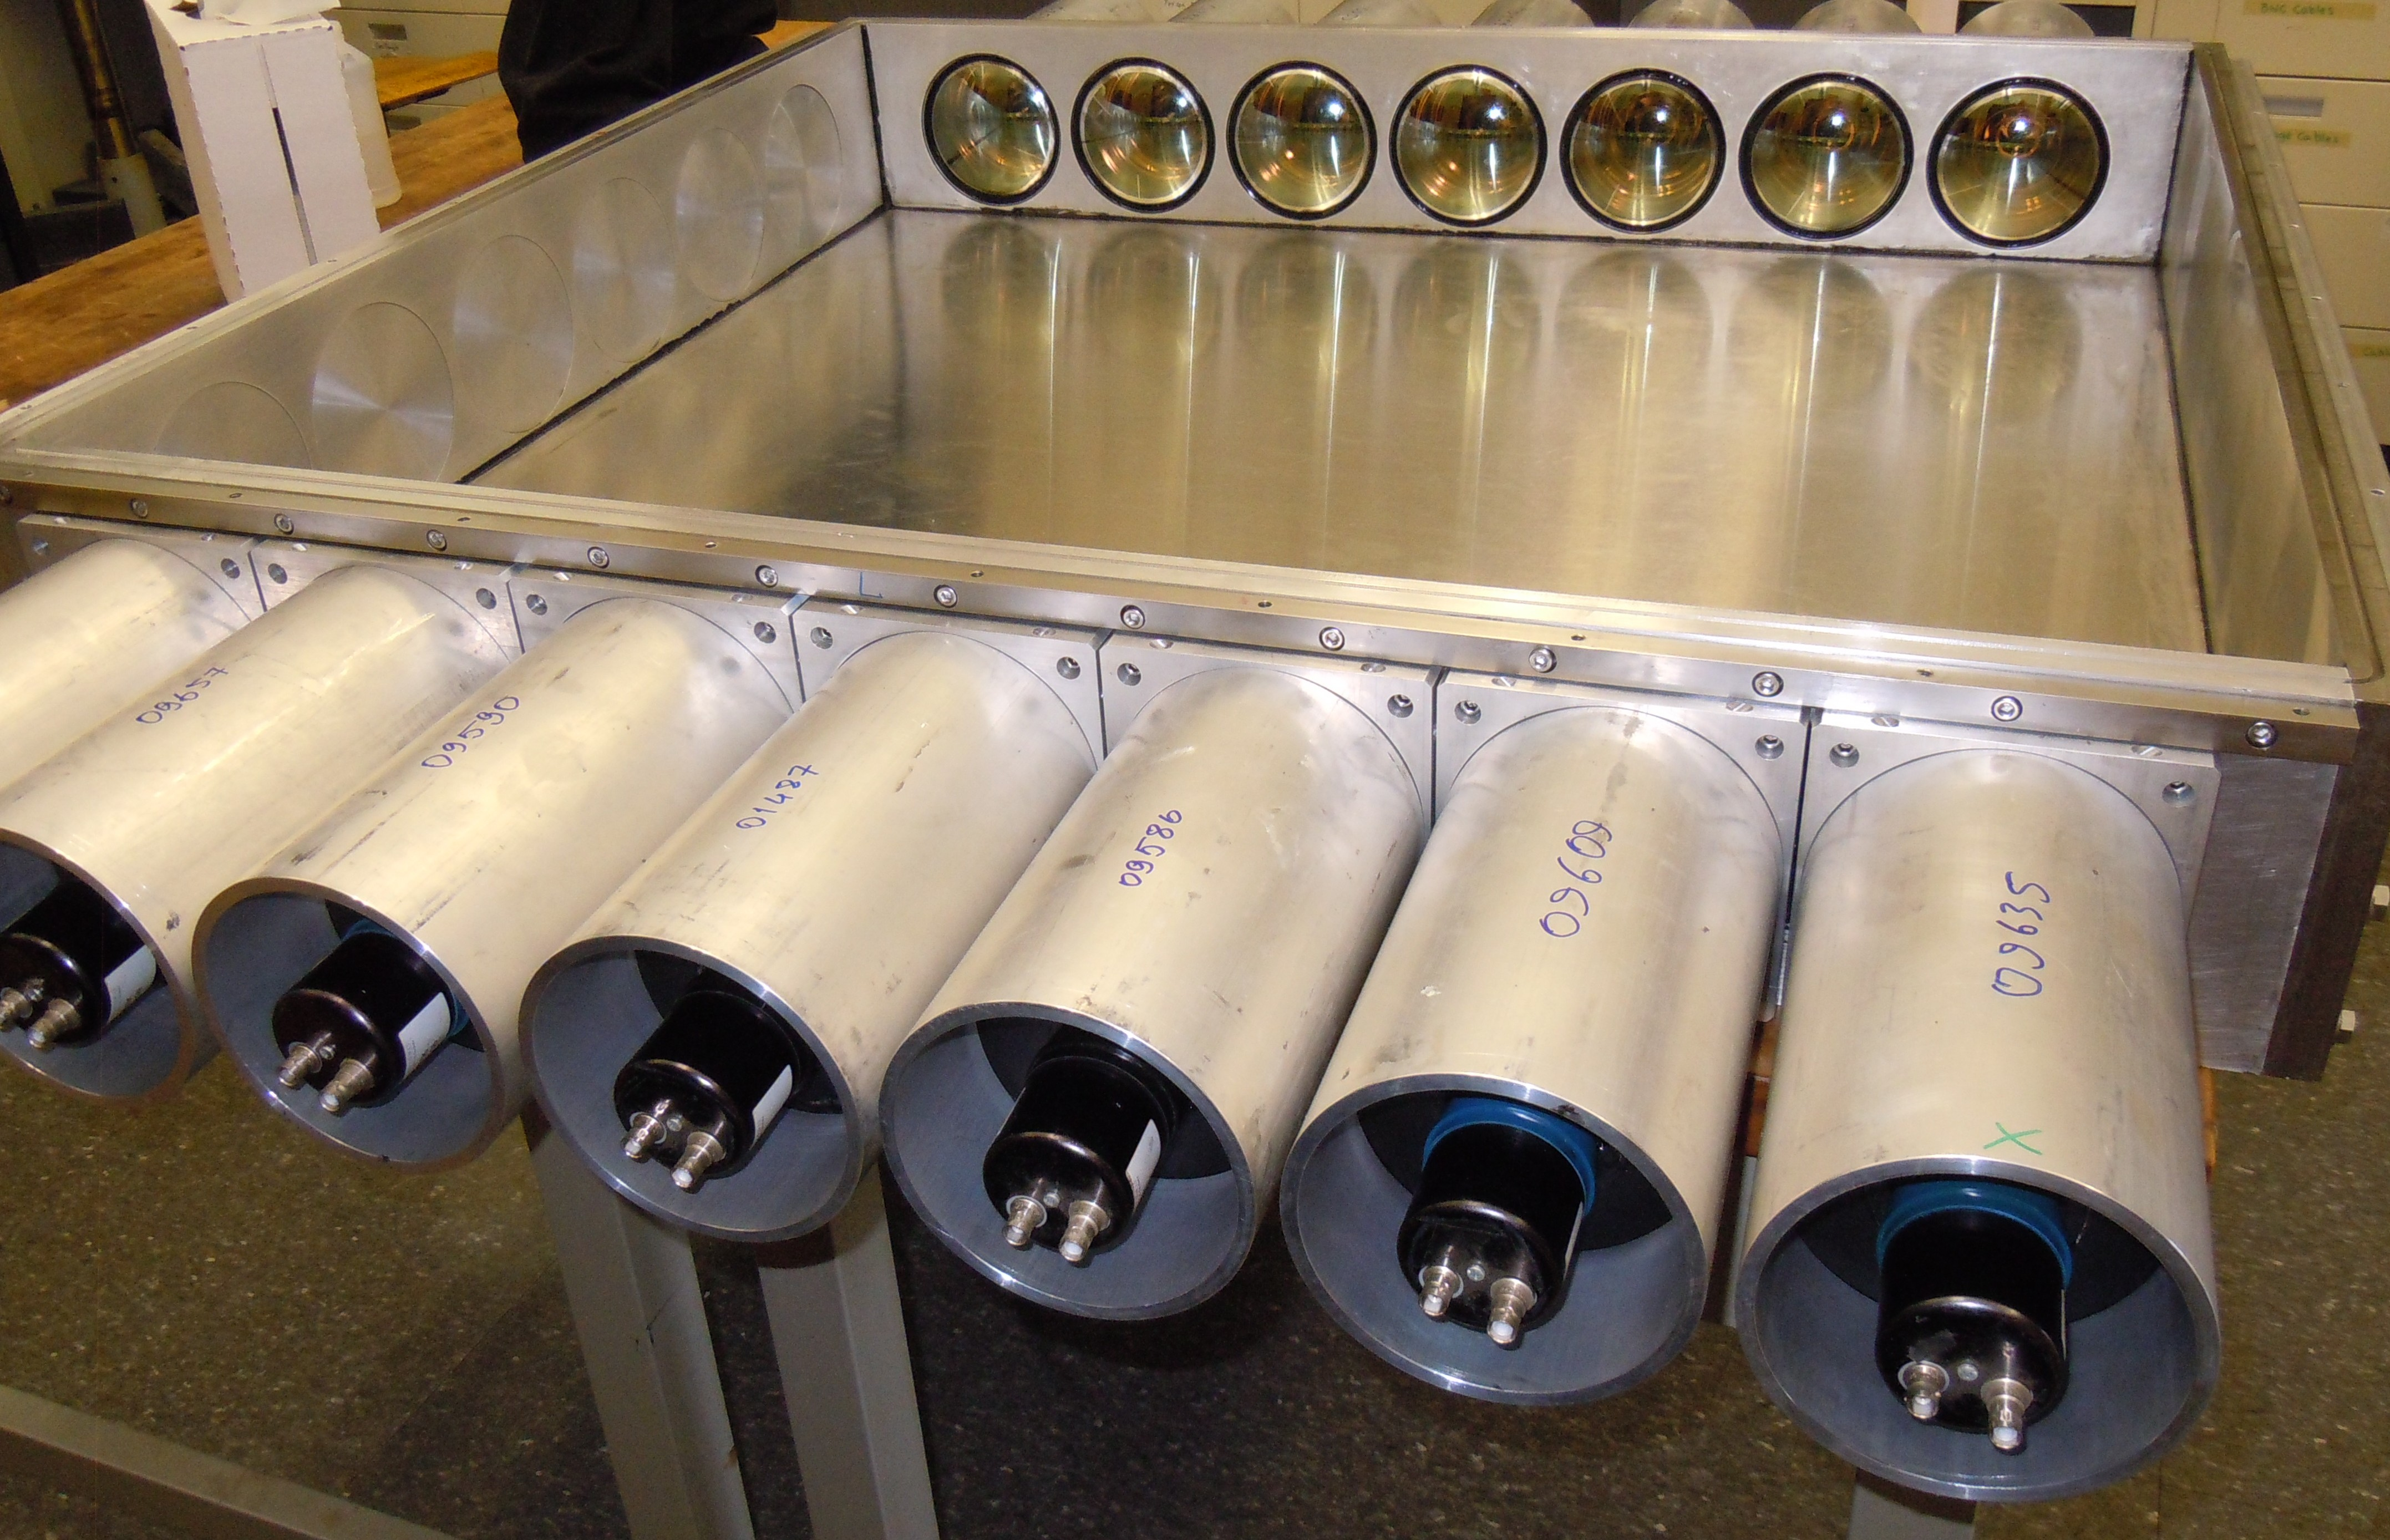
\includegraphics[width=0.5\textwidth]{chap3/shms_aerogel_open.jpg}
    \caption{The SHMS Aerogel Chereknov }
    \label{fig:shms_aerogel}
\end{figure}

The SHMS Aerogel Cherenkov~\cite{Horn_2017} was designed for K/p separation.

\subsection{Calorimeters}
A lead glass calorimeter provides another means for discriminating between
electrons and hadrons.
The calorimeters in both spectrometers consist of lead blocks with
PMTs attached that collect light generated by electromagnetic showers.
The electric field of the nuclei in the block will slow down a high energy
electron passing through the block.
The electron will radiate Bremsstrahlung photons, which will in turn generate
positron-electron pairs that will also radiate photons, and so on.
The resulting electromagnetic shower of photons, electrons, and positrons
generates Cherenkov radiation that is collected by PMTs mounted on the ends
of the lead glass blocks.
The amount of light collected is proportional to the deposited energy.
Electrons, positrons, and photons will deposit all of their energy.
For the kinematics of E12-06-102, this is between 2 and
\SI{6}{\giga\electronvolt}.
These particles will produce a peak centered around 1 in the distribution of
the track-normalized energy deposition, $E/p$.
A pion, whose mass is much greater than an electron's, will typically deposit
about \SI{300}{\mega\electronvolt}.
A negative pion undergoing a charge-exchange reaction in the bulk of the
calorimeter can produce a neutral pion which will decay into two photons,
resulting in a significant fraction of energy being deposited.
As a result, there is a large pion tail in the $E/p$ distribution that extends
up to 1.
Heavier hadrons typically deposit no energy.

\begin{figure}[ht]
    \centering
    \begin{subfigure}[b]{0.35\textwidth}
        \centering
        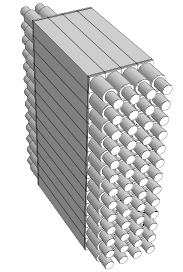
\includegraphics[width=\textwidth]{chap3/hms_calorimeter_drawing_lores.png}
        \caption{HMS calorimeter}
        \label{fig:hms_calorimeter}
    \end{subfigure}
    \hfill
    \begin{subfigure}[b]{0.35\textwidth}
        \centering
        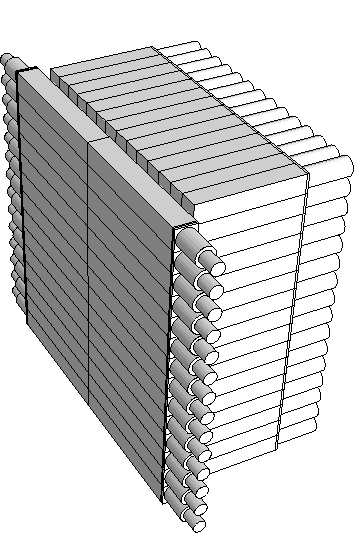
\includegraphics[width=\textwidth]{chap3/shms_calorimeter_drawing.png}
        \caption{SHMS calorimeter}
        \label{fig:shms_calorimeter}
    \end{subfigure}
    \caption{The HMS and SHMS calorimeters}
    \label{fig:calorimeters}
\end{figure}

\subsubsection{HMS Calorimeter}
The HMS calorimeter~\cite{Mkrtchyan_2012} consists of four rows of thirteen
10x10x70 \si{\cm\cubed} lead glass blocks.
The total thickness is $\sim$14.6 radiation lengths.
The blocks are made of TF-1 type lead glass with an index of refraction of
1.65, radiation length 2.74 \si{cm}, and density 3.86 \si{\gram\per\cm\cubed}..
Each block is wrapped in 25 \si{\um} thick aluminized Mylar and 40
\si{\um} thick Tedlar type film to block external light.
The light generated in each block is collected by two Phillips XP3462B PMTs,
one on each end.

\subsubsection{SHMS Calorimeter}
The SHMS calorimeter consists of a preshower and shower section.
The preshower radiator consists of one layer of 28 TF-1 type lead glass blocks,
identical to the HMS blocks, stacked in two columns of 14 blocks.
The ``fly eye'' shower array consists of 224 modules from the decommissioned
HERMES detector~\cite{Avakian_1998} stacked in 14 columns and 16 rows.
The HERMES blocks are 8.9x8.9x50 \si{\cm\cubed} blocks of F-101 type lead glass with
an index of refraction of 1.65, radiation length 2.78 \si{\cm}, and density
3.86 \si{\gram\per\cm\cubed}.
Each preshower block is read out by one Phillips XP3462B PMT, and each shower
block by one Photonis XP3461 PMT.

\section{Trigger and Data Acquisition Systems}
\label{sec:daq}

The signals from each detector's PMTs (or in the case of the drift chambers,
each wire) are digitized by ADC250~\cite{fADC_manual} flash analog-to-digital
converters (fADCS) or CAEN V1190~\cite{CAEN_1190_manual} time-to-digital
converters (TDCs).
% TODO: describe fADC mode 9 output (pulse pedestal, amplitude, integral, time)

The HMS detector hut contains a VXS crate with TDCs that process signals from
the HMS drift chambers.
The SHMS detector hut contains a VXS crate with fADCS that process signals from
the SHMS calorimeter's preshower and shower PMTs, and a VME crate with TDCs
that process signals from the SHMS drift chambers.
The Counting Room contains TDCs and fADCs to process signals from all the other
detectors, as well as sums of signals from other detectors.
These sums form ``pretrigger'' signals that are sent to a Trigger Interface
(TI) module which then distributes a specified trigger signal to synchronize
readout of the fADCs and TDCs in every read-out controller (ROC).
This analog trigger signal is called a ``Level 1 Accept,'' or L1 for short.
A copy of the Level 1 pretrigger is sent to every ROC which, when subtracted
from the raw TDC time, improves timing resolution from $\sim$\SI{25}{ns} to
$\sim$\SI{0.1}{ns}.
Both spectrometers have a TI, allowing them to be run independently or in
coincidence.


A broad overview of the SHMS trigger and readout system is given
in~\ref{fig:trigger_block_diagram}.
The HMS system is similar in structure, the largest differences being in in the
calorimeter signal chain.

% TODO: fix Cherenkov in diagram. The split signal goes to the fADC and analog
% sum. The sum goes to the fADC and to a discriminator. The bottom
% discriminator leg shouldn't be there.
\begin{figure}[!h]
    \centering
    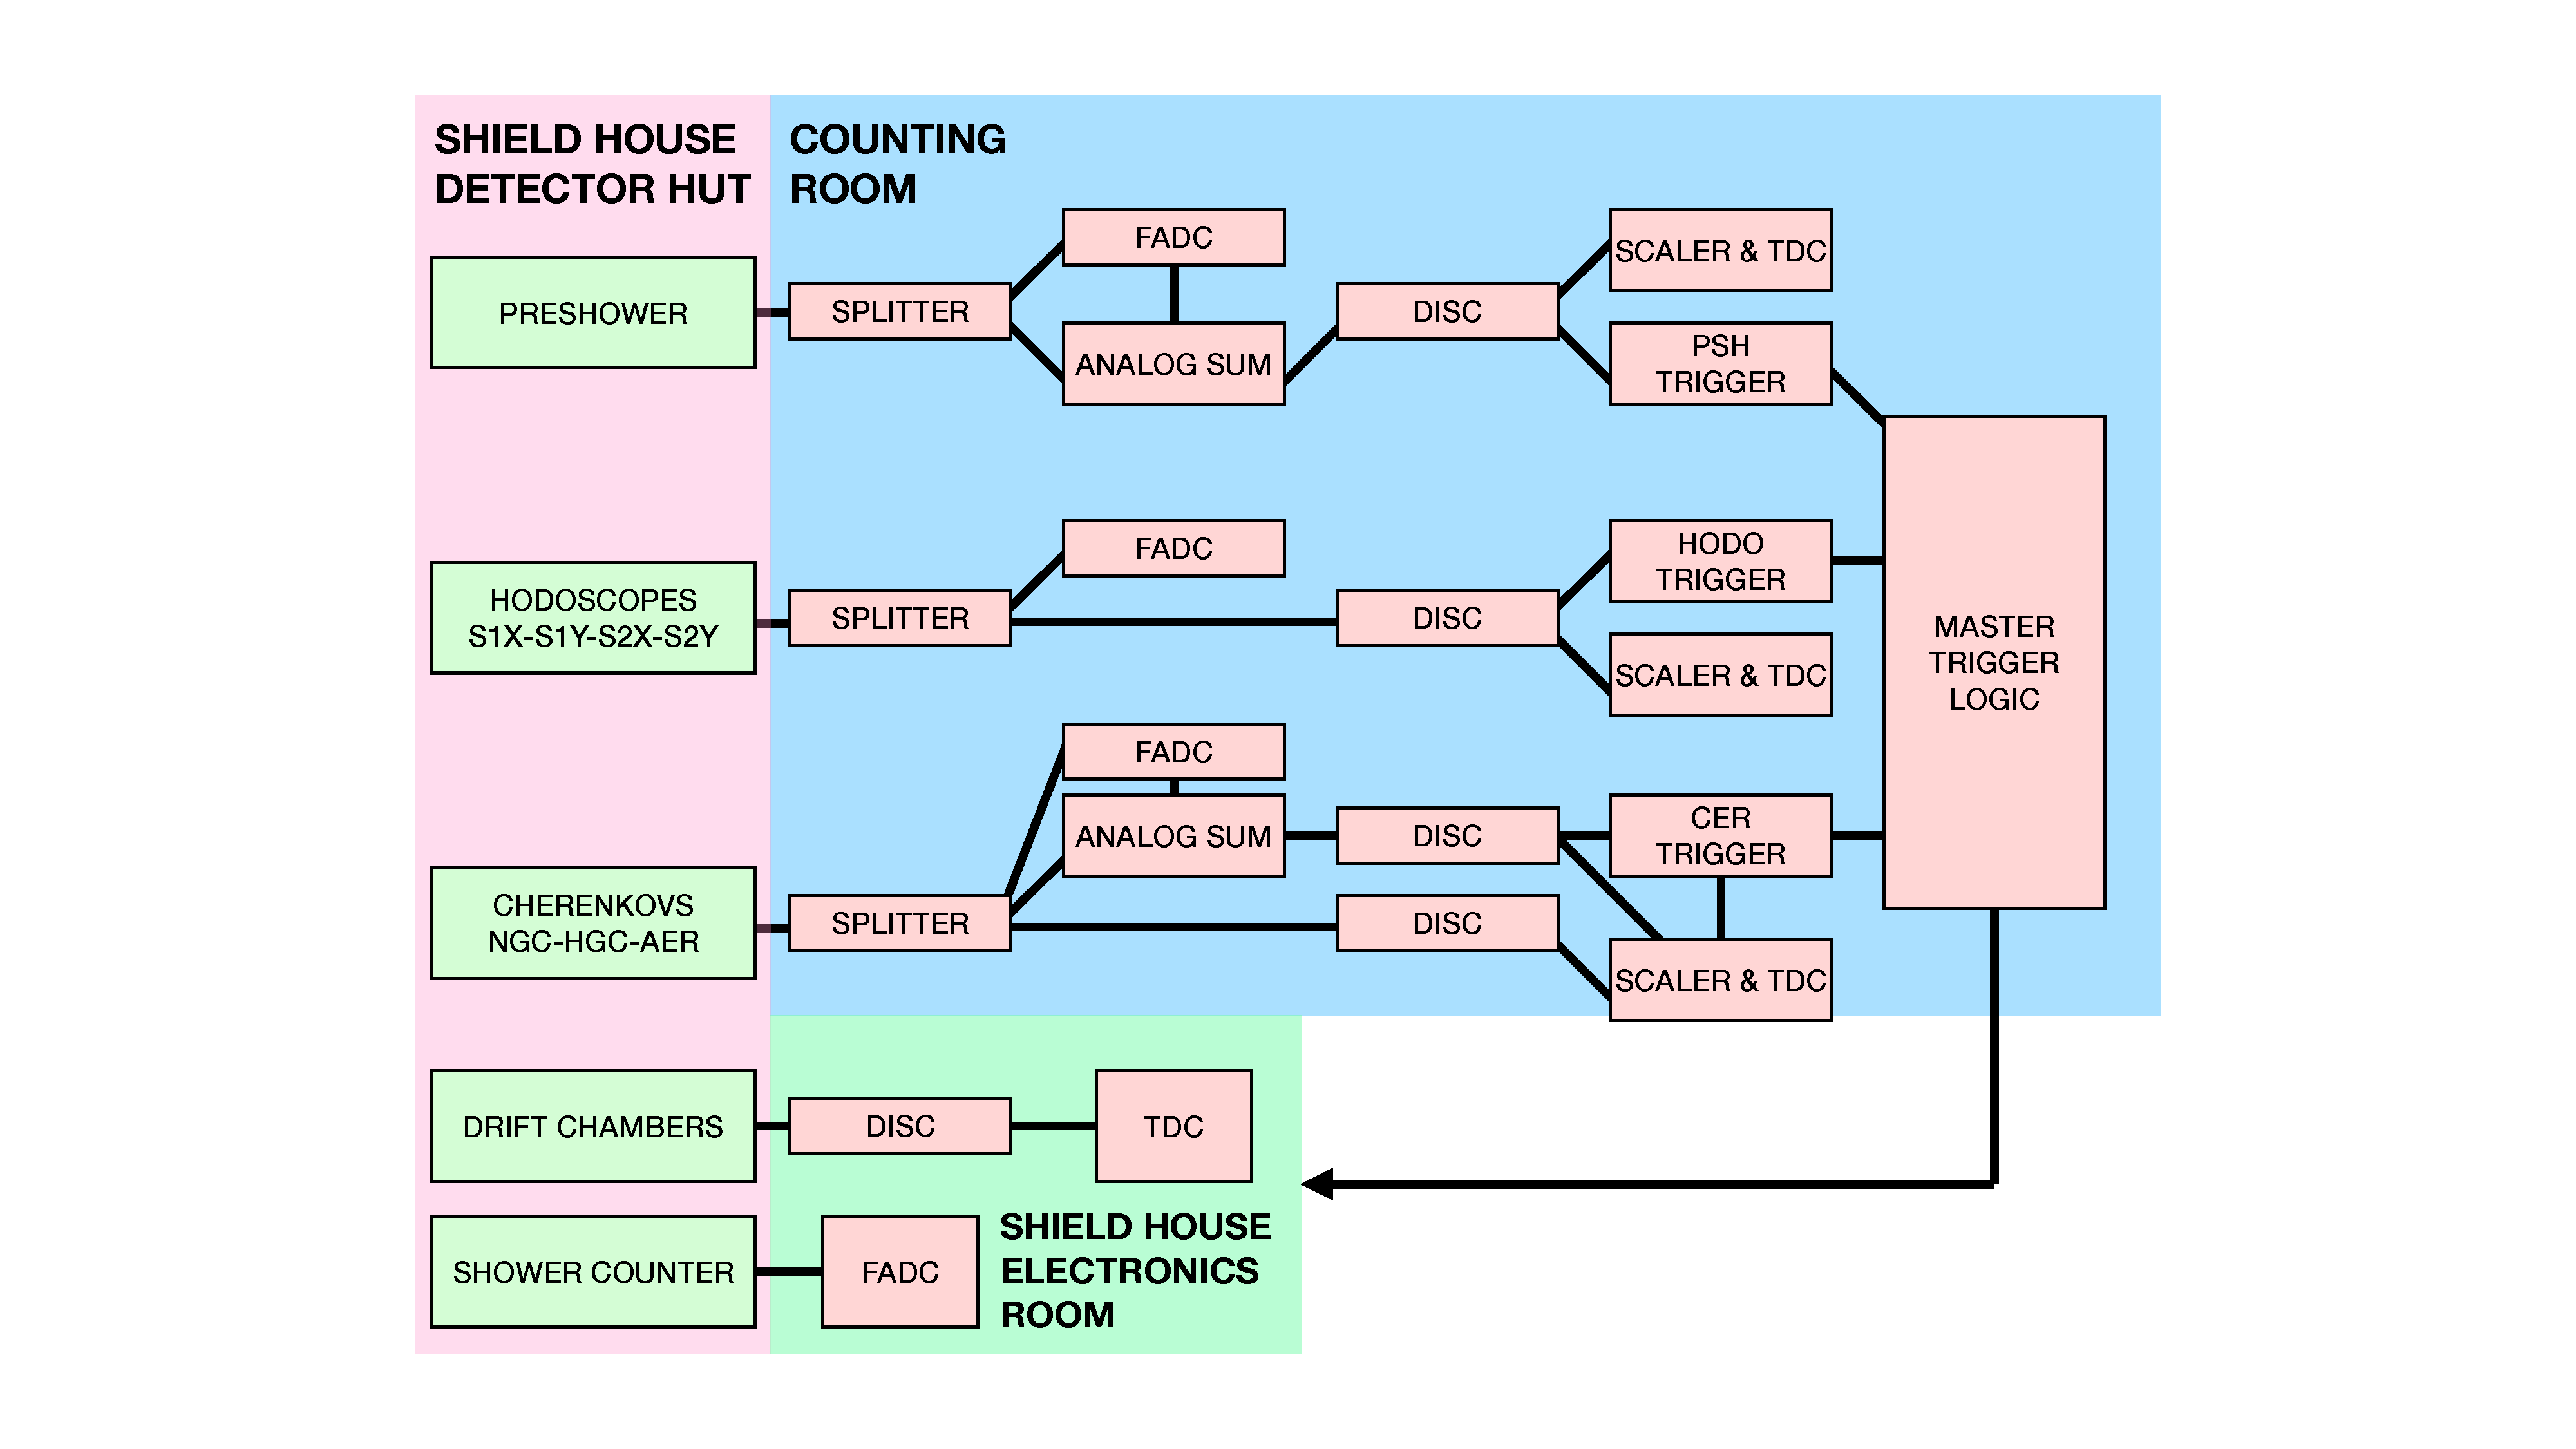
\includegraphics[width=0.9\textwidth]{chap3/trigger_block_diagram.pdf}
    \caption{Schematic diagram of the trigger system.
             Adapted from H. Fenker and B. Sawatzky.
             }
    \label{fig:trigger_block_diagram}
\end{figure}

Every trigger and pretrigger described below is sent to TDCs to keep track of
timing information necessary for event reconstruction, and scalers that count
every trigger with negligible deadtime.

\subsection{Pretriggers, TDC, and fADC Logic}
\subsubsection{Hodoscope}
Each hodoscope consists of 4 planes of scintillator paddles, with a PMT mounted
on both sides of each paddle.
The signal from each PMT is sent to a passive splitter.
One third of the signal amplitude is sent to an fADC, and the other two thirds
are sent to a discriminator.
The discriminator outputs are sent to daisy-chained TDCs and scalers, as well
as a LeCroy 4564 logic unit.
The logic unit computes a per-plane pretrigger by taking the AND of both sides'
$N$-fold ORs of each side's $N$ PMTs.
For instance, let h1X+ denote the 16-fold OR of the 16 PMTs on the left side of
the 1X plane of the HMS hodoscope and similarly h1X- denote the equivalent OR
of the right hand side.
Then the h1X plane pretrigger is the AND of h1X+ and h1X-.
The equations below describe the logic of each plane of the HMS and SHMS
hodoscopes' pretriggers\footnote{Because the SHMS 2Y plane has more PMTs than
each logic unit has channels, each side's 21-fold OR is actually an OR of a
16-fold OR and a 5-fold OR.}.
\begin{align*}
    \text{h1X = h1X+ (16-fold OR) AND h1X- (16-fold OR)} \\
    \text{h1Y = h1Y+ (10-fold OR) AND h1Y- (10-fold OR)} \\
    \text{h2X = h2X+ (16-fold OR) AND h2X- (16-fold OR)} \\
    \text{h2Y = h2Y+ (10-fold OR) AND h2Y- (10-fold OR)}
\end{align*}
\begin{align*}
    \text{p1X = p1X+ (13-fold OR) AND p1X- (13-fold OR)} \\
    \text{p1Y = p1Y+ (13-fold OR) AND p1Y- (13-fold OR)} \\
    \text{p2X = p2X+ (14-fold OR) AND p2X- (14-fold OR)} \\
    \text{p2Y = p2Y+ (21-fold OR) AND p2Y- (21-fold OR)}
\end{align*}

These pretriggers are converted from ECL twisted-pair to NIM signals by sets of
P/S model 7126 16-channel logic level translators~\cite{PS7126_manual}.
The NIM pretrigger signals are converted to variable-width gates by sets of P/S
model 752 logic units~\cite{PS752_manual}.
Sets of P/S Model 755 logic units~\cite{PS755_manual} generate the following
pretriggers for both spectrometers based on concidences of hodoscope plane
pretriggers:

\begin{itemize}
    \item S1 = 1X OR 1Y
    \item S2 = 2X OR 2Y
    \item STOF = S1 AND S2
    \item HODO 3/4 = coincidence of at least 3 planes
\end{itemize}

\subsubsection{Calorimeters}
Both spectrometer's calorimeters consist of two (SHMS) to four (HMS) layers of
long lead-glass blocks connected to PMTs on one or both sides.


The signals from the HMS calorimeter PMTs are read out in the Counting Room,
where they pass through a passive 50:50 splitter, with one half of each signal
sent to fADC inputs.
The other half is sent to P/S model 740 analog sum modules~\cite{PS740_manual}
which generate sums for each side of each layer (hA+, hA-, hB+, hB-, hC, and
hD\footnote{The third and fourth layers of the HMS calorimeter only have PMTs
connected to one side.}).
A LeCroy model 428F~\cite{LeCroy428F_manual} module sums both sides of the
first two layers to form hA and hB.
Each layer's sum is then sent to an fADC as well as a P/S model 715
discriminator~\cite{PS715_manual} to form the following calorimeter
pretriggers:

\begin{itemize}
    \item hPreSH LO = hA < \SI{-40}{mV}
    \item hPreSH HI = hA < \SI{-60}{mV}
    \item hShower LO = hA + hB + hC + hD < \SI{-45}{mV}
\end{itemize}


The SHMS calorimeter shower counter PMTs are all sent directly to fADCs inside
the electronics hut.
As in the HMS, each SHMS preshower layer PMT's output passes through a passive
50:50 splitter, with half the signal amplitude sent to an fADC and the other
half sent to analog sum modules that generate preshower LO/HI pretriggers.

\subsubsection{Cherenkovs}
All the threshold Cherenkov detectors in both spectrometers consist of some
medium in (some types of) charged particles generate Cherenkov radiation in the
visible spectrum and some number of PMTs that collect this light.
The output of each PMT is read out in the Counting Room, where it passes
through a passive 50:50 splitter.
One half of the signal amplitude is sent to an fADC, and the other half is sent
to a LeCroy 428F summing module~\cite{LeCroy428F_manual}.
This sum is sent to an fADC as well as to a P/S model 715
discriminator~\cite{PS715_manual} to form a pretrigger for that Cherenkov

\subsubsection{Other Pretriggers}
Four other pretrigger signals are generated from combinations of pretrigger
signals described above.
They are as follows:

\begin{itemize}
    \item EL-Hi = (HODO 3/4) AND (PreSH HI)
    \item EL-Lo = (Two of three from {HODO 3/4, STOF, PreSH LO}) AND (Cer)
    \item EL-Real = EL-Hi OR EL-Lo
    \item EL-Clean = EL-Hi AND EL-Lo
\end{itemize}

\subsubsection{Electronic Dead Time Measurement (EDTM) Pulser}
\label{sec:edtm}
To estimate the deadtime due to all electronics involved in data acquisition, a
pulser with a low frequency (\SI{3}{\hertz} in our experiment) is inserted into the
trigger logic.
The EDTM pulser fires every trigger in the system, and is also sent to its own
TDC and scaler channels.
By comparing the number of accepted EDTM triggers to the number of EDTM trigger
counts seen by the scaler, one can estimate deadtime.
This process is discussed in more detail in Section~\ref{sec:livetime}.

\subsection{Reference Times}
The reference time for an event is an OR-ed version of pretrigger signals
distributed to each fADC and TDC in every ROC.
The TDC modules have two internal clocks, one with a \SI{40}{MHz} cycle and one
with a \SI{10}{GHz} cycle.
When a given detector signal is received by a TDC, the digitized time latches
onto the leading edge of the 40 MHz cycle, yielding a timing resolution of
$\sim$\SI{25}{ns}.
We feed a \textit{reference time}, a copy of the pretrigger (common to all
fADCs and TDCs in a given ROC), to the TDC which will latch onto the leading
edge of the faster \SI{10}{GHz} clock.
The \textit{hcana} analyzer subtracts the reference time from detectors' raw
TDC times to yield a timing resolution of $\sim$\SI{0.1}{ns}.
This process is discussed in more detail in Section~\ref{sec:reftime}.


\chapter{Data Analysis}

\input{chap4/introduction}
\section{Detector Calibrations}
% TODO: make sure I have links to calibration guides for each system
\subsection{Hodoscopes}
The calibration procedure for the hodoscopes consists of determining a set of
timing corrections applied to the raw times $t_{raw}$ generated by
discriminators fed into TDCs.
The general form of a corrected TDC time for one end of a scintillator paddle
is
\begin{equation}
    t_{corr} = t_{raw} - t_{TW} - t_{cable} - t_{prop} - t_{\lambda}
\end{equation}

\begin{itemize}
    \item \textbf{Timewalk corrections} $t_{TW}$

Timewalk refers to the correlation between
the amplitude of an analog signal fed into a leading-edge, fixed-threshold discriminator
and the time the signal rises rises above the discriminator's threshold.
As seen in Fig~\ref{fig:pooser_timewalk}, pulses with a smaller amplitude cross
a fixed threshold at later times despite starting at the same time.

\begin{figure}[!h]
    \centering
    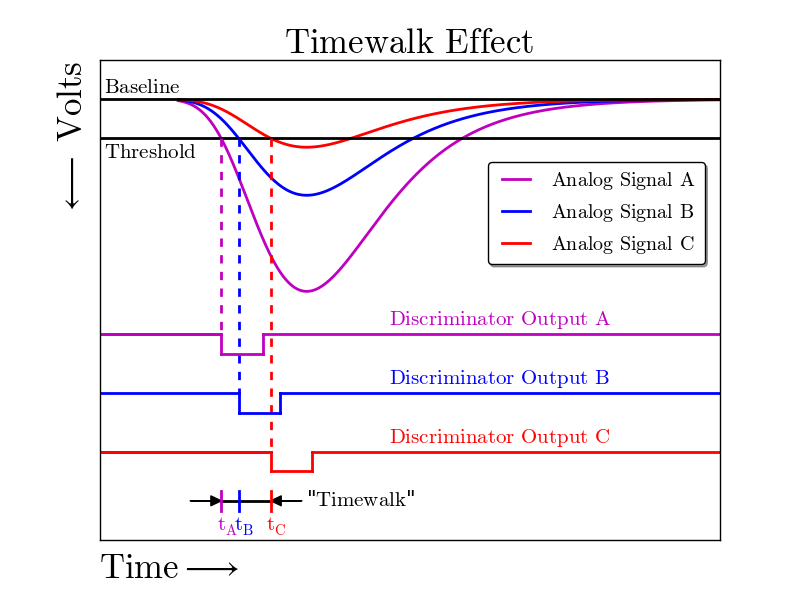
\includegraphics[width=0.6\textwidth]{chap4/pooser_timewalk.png}
    \caption{
            An illustration of the timewalk effect.
            Pulses with a smaller amplitude cross the fixed threshold at a
            later time.
            The TDCs in the Hall C DAQ are prone to this effect.
            }
    \label{fig:pooser_timewalk}
\end{figure}

Fortunately, the fADCs are not prone to this effect so the pulse time recorded
by an fADC can be used to correct the corresponding TDC time.
The fADC pulse time is determiend by a constant fraction discriminator (CFD)
algorithm that finds the time,
to a precision of \SI{62.5}{\pico\second},
at which the pulse reaches 50\% of its maximum amplitude.
This algorithm is illustrated in Fig~\ref{fig:pooser_cfd}, and a comparison of
pulse times of varying amplitudes is shown in Fig~\ref{fig:pooser_notimewalk}.

\begin{figure}[!h]
    \centering
    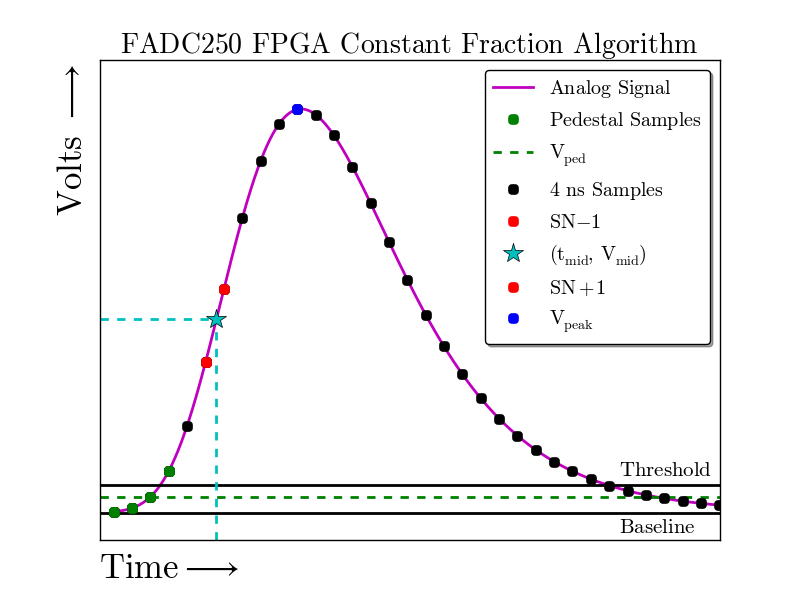
\includegraphics[width=0.6\textwidth]{chap4/pooser_cfd.png}
    \caption{
            An illustration of the fADCs' CFD algorithm.
            The algorithm calculates the pedestal amplitude $V_{ped}$ with a
            fixed-threshold discriminator.
            It then calculates the half-amplitude $V_{mid}=(V{peak}-V_{ped})/2$
            and determines which two samples $SN-1$ and $SN+1$ lie on either
            side of $V_{mid}$.
            The fADCs' coarse sampling rate is \SI{250}{\mega\hertz}, yielding
            \SI{4}{\nano\second} between the two samples.
            This time is divided into 64 subsamples of \SI{62.5}{\pico\second}
            each, and the time $t_{mid}$ corresponding to $V_{mid}$ is found by
            linear interpolation..
            }
    \label{fig:pooser_cfd}
\end{figure}

\begin{figure}[!h]
    \centering
    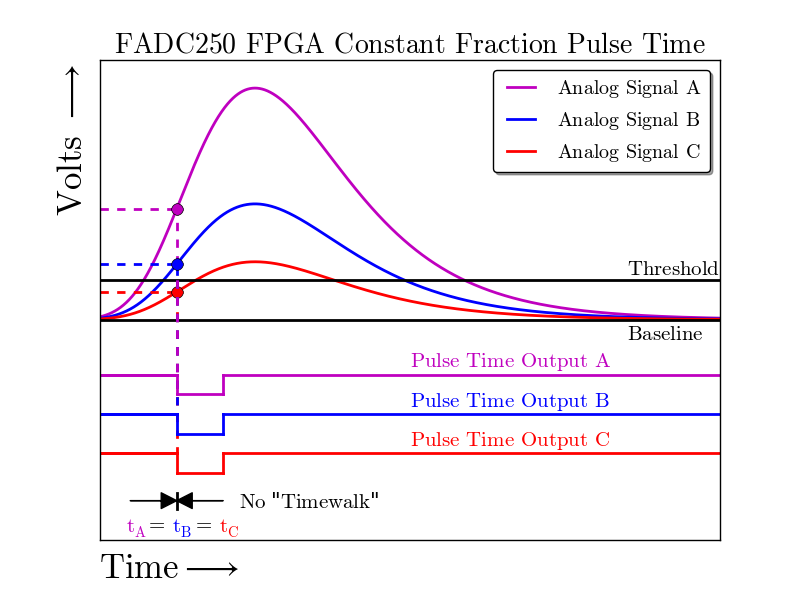
\includegraphics[width=0.6\textwidth]{chap4/pooser_notimewalk.png}
    \caption{
            An illustration of the absence of timewalk in the fADCs' CFD algorithm.
            }
    \label{fig:pooser_notimewalk}
\end{figure}

A plot of the difference between raw TDC time and fADC pulse time
versus fADC pulse amplitude can be fit to the form
$t_{TW}(a) = c_1 + \frac{1}{\frac{a}{TDC_{thr}}c2}$
where $a$ is the pulse amplitude and
$TDC_{thr}$ is the TDC threshold (\SI{120}{\milli\volt} in this experiment).
The per-PMT parameters $c_1$ and $c_2$ are extracted from a calibration run
with large statistics.

\begin{figure}[!h]
    \centering
    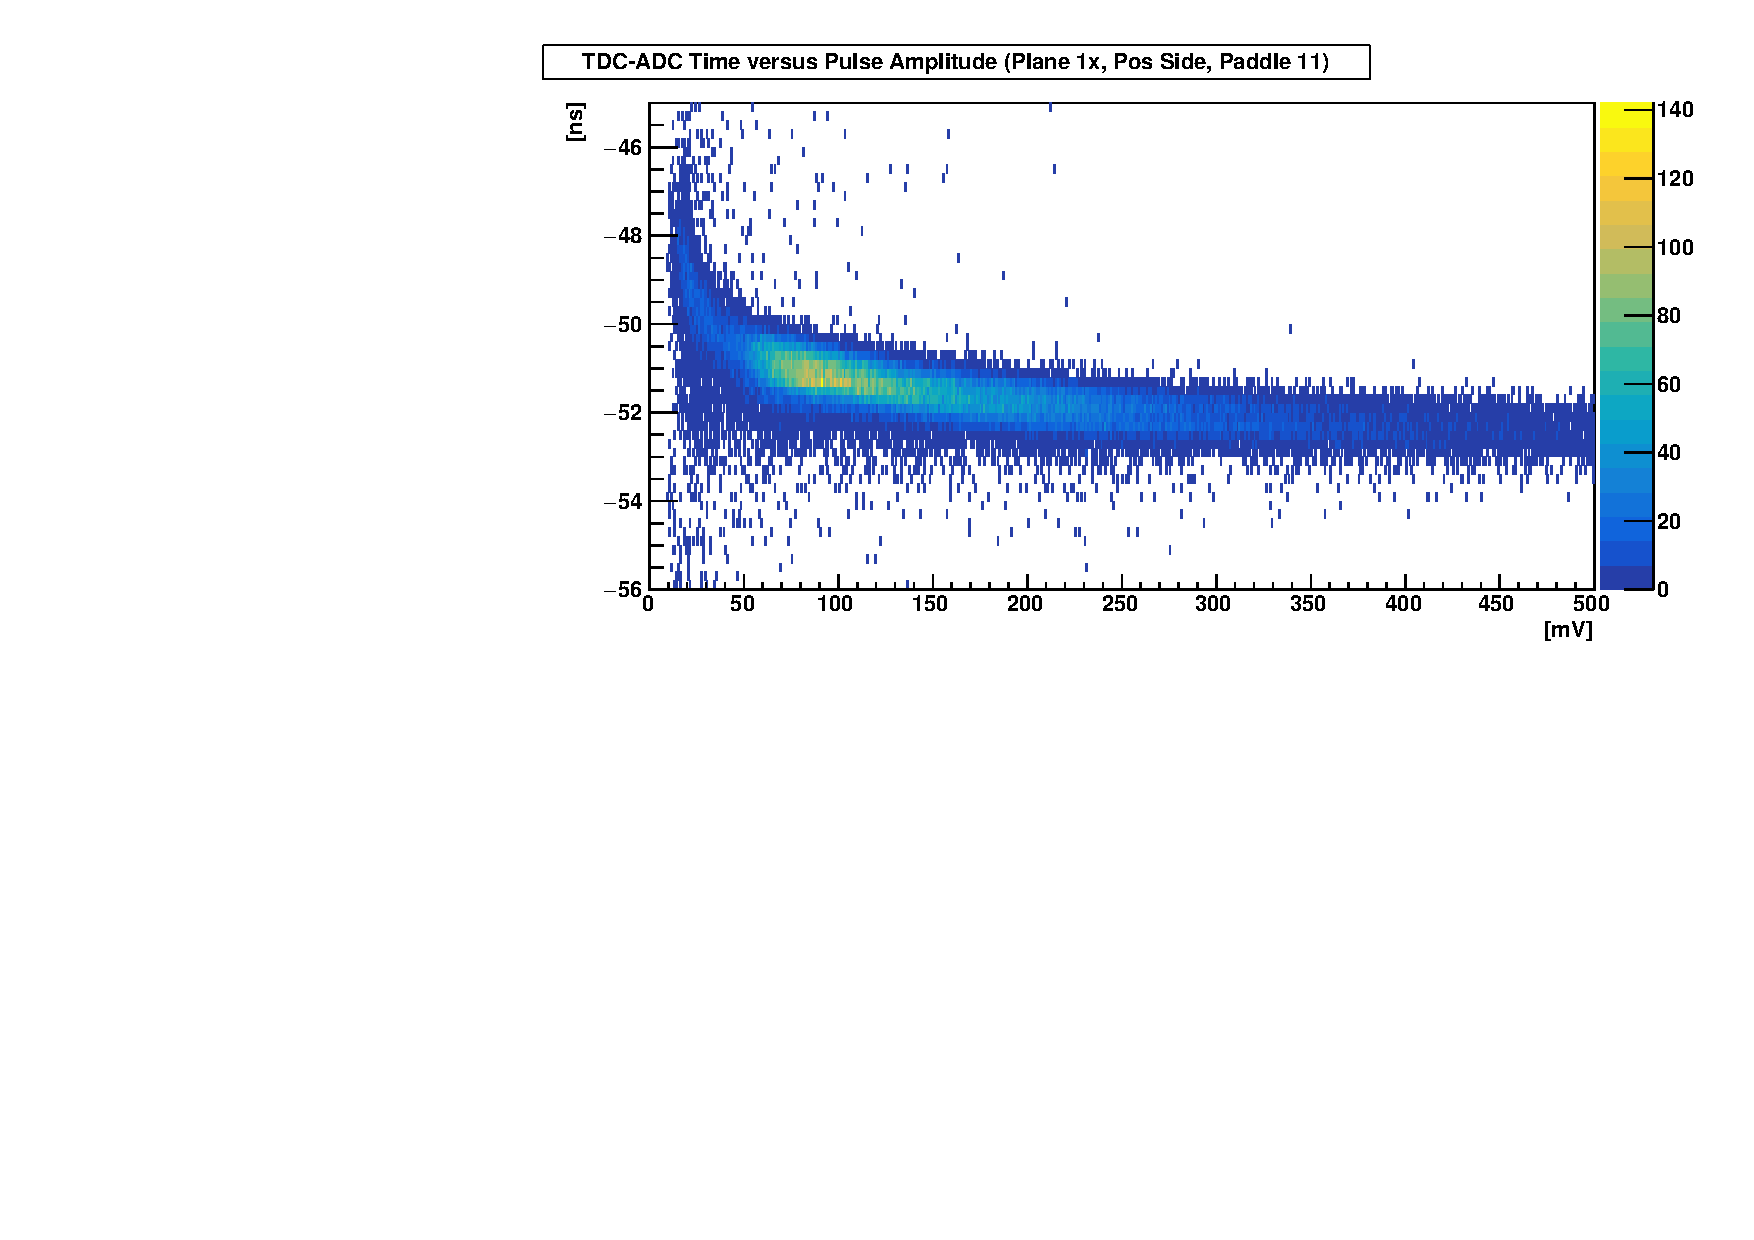
\includegraphics[width=1.0\textwidth]{chap4/plot_scripts/hodo_timewalk.pdf}
    \caption{
            A two dimensional histogram showing the difference between TDC
            and fADC pulse times as a function of fADC pulse amplitude.
            As shown in Fig~\ref{fig:pooser_timewalk}, smaller pulses cross a
            fixed threshold at a later time, leading to a delayed TDC time.
            }
    \label{fig:time_walk_histogram}
\end{figure}


    \item \textbf{Cable/light propagation time} $t_{cable}$, $t_{prop}$

Signals from the hodoscope travel through BNC cables from the detector hut
underground up to the electronics racks in the counting house above ground.
Differences in cable propagation time between the opposite ends of the paddles
need to be accounted for.
The timewalk-corrected TDC times for the $+$ and $-$ sides of a paddle are
the sum of the propagation time for the light through the paddle
and the propagation time through the cables,
$t^{\pm}=t^{\pm}_{prop}+t^{\pm}_{cable}$.
The difference between the $+$ and $-$ sides' times should be proportional to
the track's distance from the center of the paddle
% TODO: not actually $y$, but distance from center. clarify this.
(i.e. the $y$ coordinate for a horizontal paddle, $x$ for a vertical paddle).
If $v$ is the speed of light in the paddle, this difference is
$\Delta t = \frac{y}{v} + b$,
where $b$ is a parameter that captures the offset due to differences in cable
propagation time.
A linear fit of the time difference $\Delta t$ versus track distance from the
center of the paddle is used to extract the cable offset and light propagation
speed for each paddle.
The intercept $b$ is the cable propagation time correction $t_{cable}$
and the slope $1/v$ determines the light propagation time correction
$t^\pm_{prop}$.
For a horizontal paddle,
$t^\pm_{prop} = (\pm L_\pm \pm y_{hit})$
where $L_\pm$ is the $y$ coordinate of the ends of the paddle and
$y_{hit}$ is the $y$ coordinate of the particle's track projected to the
paddle's $z$ position.
The same formula holds for a vertical paddle, but using $L_\pm$ in the $x$
direction and $x_{hit}$ at the paddle's $z$ position.

    \item \textbf{Small perturbations} $t_{\lambda}$

This term corrects for small differences $\lambda$ in timing between planes.
Let $t_i$ be the time, corrected for timewalk and propagation time,
of a hit on a paddle in plane $i$,
and $D_{ij}$ be the distance between planes $i$ and $j$.
Then the difference between hits in these planes with small perturbations can
be expressed as
\begin{equation}
    (t_i+\lambda_i) - (t_j+\lambda_j) = \frac{D_{ij}}{v}
\end{equation}
or equivalently, defining a term $b_{ij}$,
\begin{equation}
    \lambda_i - \lambda_j = \frac{D_{ij}}{v} - (t_i - t_j) \equiv b_{ij}
\end{equation}

Generalizing this to all 6 combinations of differences between 4 planes, we can
set up a system of linear equations with coefficients $c_i,j=\pm1$ where $i$
represents one of the 6 plane combinations and $j$ is the ``absolute'' paddle
number.
Paddles are indexed with $j$ from 1 to the total number of paddles in the
4 planes.
In the HMS there are 52 total paddles, so the system of linear equations is

\begin{align}
    c_{1,1}\lambda_1 + c_{1,2}\lambda_2 + \cdots + c_{1,52}\lambda_52 &= b_{12} \\
    c_{2,1}\lambda_1 + c_{2,2}\lambda_2 + \cdots + c_{2,52}\lambda_52 &= b_{13} \\
    c_{3,1}\lambda_1 + c_{3,2}\lambda_2 + \cdots + c_{3,52}\lambda_52 &= b_{14} \\
    c_{4,1}\lambda_1 + c_{4,2}\lambda_2 + \cdots + c_{4,52}\lambda_52 &= b_{23} \\
    c_{5,1}\lambda_1 + c_{5,2}\lambda_2 + \cdots + c_{5,52}\lambda_52 &= b_{24} \\
    c_{6,1}\lambda_1 + c_{6,2}\lambda_2 + \cdots + c_{6,52}\lambda_52 &= b_{34} \\
\end{align}

or in matrix notation

\begin{gather}
    C\vec{\lambda}
    =
    \begin{bmatrix}
        c_{1,1} & c_{1,2} & \cdots & c_{1,52} \\
        c_{2,1} & c_{2,2} & \cdots & c_{2,52} \\
        c_{3,1} & c_{3,2} & \cdots & c_{3,52} \\
        c_{4,1} & c_{4,2} & \cdots & c_{4,52} \\
        c_{5,1} & c_{5,2} & \cdots & c_{5,52} \\
        c_{6,1} & c_{6,2} & \cdots & c_{6,52} \\
    \end{bmatrix}
    \left[ \begin{array}{c} \lambda_1 \\ \lambda_2 \\ \vdots \\ \lambda_{52} \end{array} \right]
    =
    \left[ \begin{array}{c} b_{12} \\ b_{13} \\ b_{14} \\ b_{23} \\ b_{24} \\ b_{34}  \end{array} \right]
\end{gather}

Solving this for all $\lambda$s requires accumulating statistics from a run with
many events $k$:
\begin{gather}
    C\vec{\lambda}
    =
    \begin{bmatrix}
        \sum_k c_{1,1} & \sum_k c_{1,2} & \cdots & \sum_k c_{1,52} \\
        \sum_k c_{2,1} & \sum_k c_{2,2} & \cdots & \sum_k c_{2,52} \\
        \sum_k c_{3,1} & \sum_k c_{3,2} & \cdots & \sum_k c_{3,52} \\
        \sum_k c_{4,1} & \sum_k c_{4,2} & \cdots & \sum_k c_{4,52} \\
        \sum_k c_{5,1} & \sum_k c_{5,2} & \cdots & \sum_k c_{5,52} \\
        \sum_k c_{6,1} & \sum_k c_{6,2} & \cdots & \sum_k c_{6,52} \\
    \end{bmatrix}
    \left[ \begin{array}{c} \lambda_1 \\ \lambda_2 \\ \vdots \\ \lambda_{52} \end{array} \right]
    =
    \left[ \begin{array}{c}  \sum_k b_{12} \\  \sum_k b_{13} \\  \sum_k b_{14} \\  \sum_k b_{23} \\  \sum_k b_{24} \\  \sum_k b_{34}  \end{array} \right]
\end{gather}

\textit{hcana} solves for $\vec{\lambda}$ using singular value
decomposition, yielding a set of corrections $t_\lambda = \lambda_i$ for every
paddle $i$.

% TODO: clarify that we only used timewalk corrections

\end{itemize}

\subsection{Drift Chambers} \label{sec:dc_calib}
When a charged particle passes through the drift chambers, it ionizes the gas
filling the chamber.
The electric field generated by the field wires causes the freed electrons to
drift toward sense wires over a ``drift time'' $t_D$.
The sense wires are read out by discriminators fed into TDC channels.
Knowledge of which wires in each plane have been fired permits coarse track
reconstruction.
Finer resolution can be achieved by using the drift time to estimate a drift
distance $d_D$, the distance from the wire at which the ionization occurred.


Assuming the events used for calibration illuminate the detector uniformly
and that the drift velocity is uniform across the detector, the relationship
between drift distance and drift time $t_D$ is
\begin{equation}
    d_D (\tau=t_D) = \frac{\Delta}{2}
                     \frac{\int_{t_0}^{t_D<t_{max}} F(\tau) d\tau}
                          {\int_{t_0}^{t_{max}} F(\tau) d\tau}
\end{equation}

where $F(\tau)$ is the distribution of drift times.
The times $t_0$ and $t_{max}$ are the minimum and maximum drift times,
determined by the cell spacing and drift velocity.
They are extracted from the distribution $F(\tau)$.
The constant $\Delta/2$ ensures this expression respects the limiting cases of
particles passing immediately adjacent to a sense wire or exactly between
two sense wires.


The TDCs have a finite resolution, so these integrals are in reality actually
sums over bins $F_i$ with widths $\Delta\tau$,
\begin{align} \label{eqn:drift_distance}
    d_D (\tau=t_D) &= \frac{\Delta}{2}
                      \frac{\sum_{i=0}^{n_{max}<N} F_i \Delta\tau}
                           {\sum_{i=0}^{N} F_i \Delta\tau} \\
                 &= \frac{\Delta}{2}
                    \frac{1}{N}\sum_{i=0}^{n_{max}} F_i
\end{align}
where $i$ is the bin index,
$n$ is the index of the bin in which drift time $t_D$ lies,
and $N$ is the index of the maximum drift time.


The first step in calibrating the drift chambers is determining a $t_0$ for
every wire.
This is done by finding the point at which a linear fit of the lower range of
the drift time spectrum to cross the x axis, as shown in
Fig~\ref{fig:drift_time_fit}.
If there are insufficient per-wire statistics to obtain a good fit,
the distribution for all 16 wires connected to a card may be used instead to
obtain a per-card $t_0$.

\begin{figure}[!h]
    \centering
    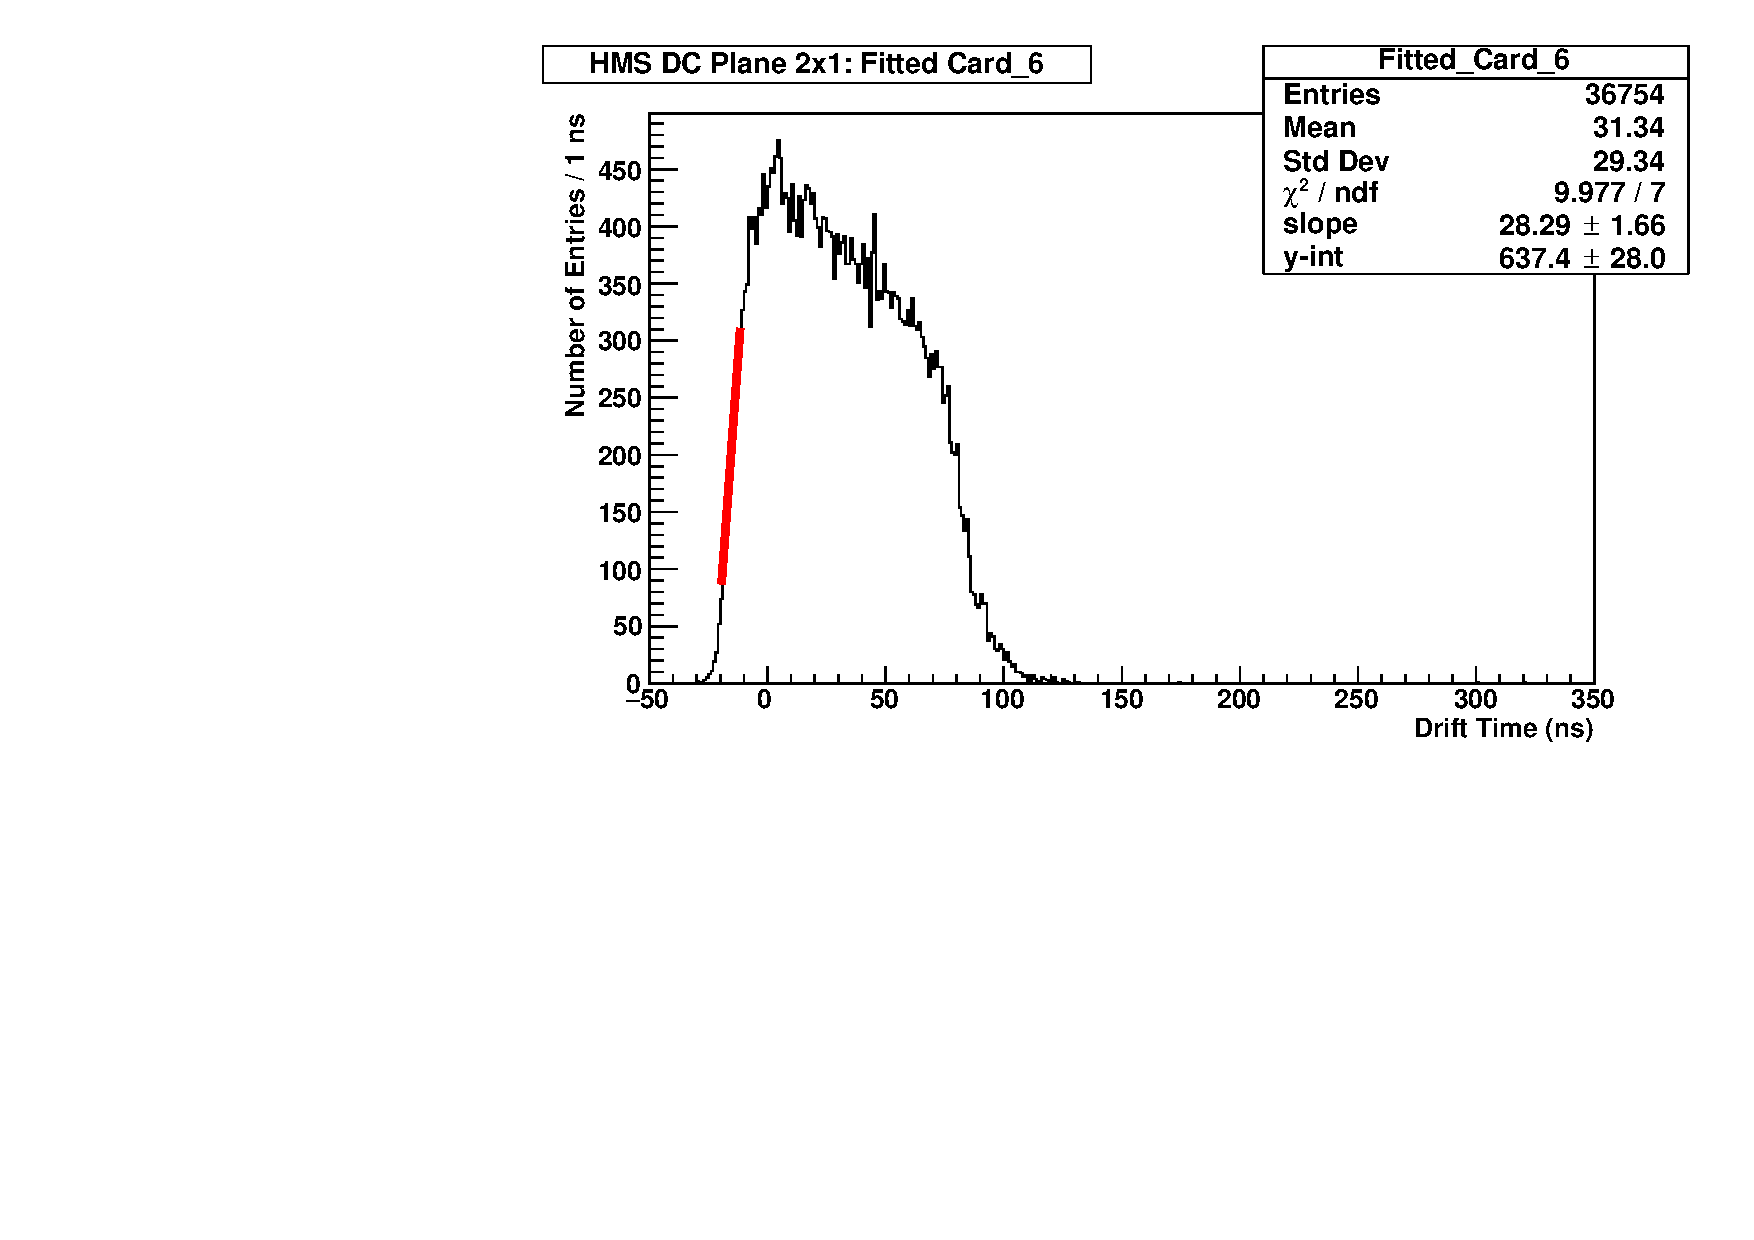
\includegraphics[width=0.8\textwidth]{chap4/drift_time_fit.pdf}
    \caption{
            The distribution of drift times for one card in the HMS 2x1 plane.
            The red line is a linear fit to the range corresponding to 20--60\%
            of the maximum bin content.
            The x-intercept of the fit is used as the offset $t_0$ for all
            wires in the card.
            }
    \label{fig:drift_time_fit}
\end{figure}

The calibration script first generates a histogram of drift times with bins of
width \SI{1}{\nano\second}
and finds the bin in the histogram containing the maximum number of entries.
A linear fit is then performed over the bins corresponding to 20--60\% of the
maximum bin content.
The x-intercept of this fit yields $t_0$, which can then be used to create a
lookup table using equation~\ref{eqn:drift_distance}.
An example of the distribution of uncorrected and corrected drift times is
shown in Fig~\ref{fig:drift_th2s}.

\begin{figure}[ht]
    \centering
    \begin{subfigure}[b]{0.8\textwidth}
        \centering
        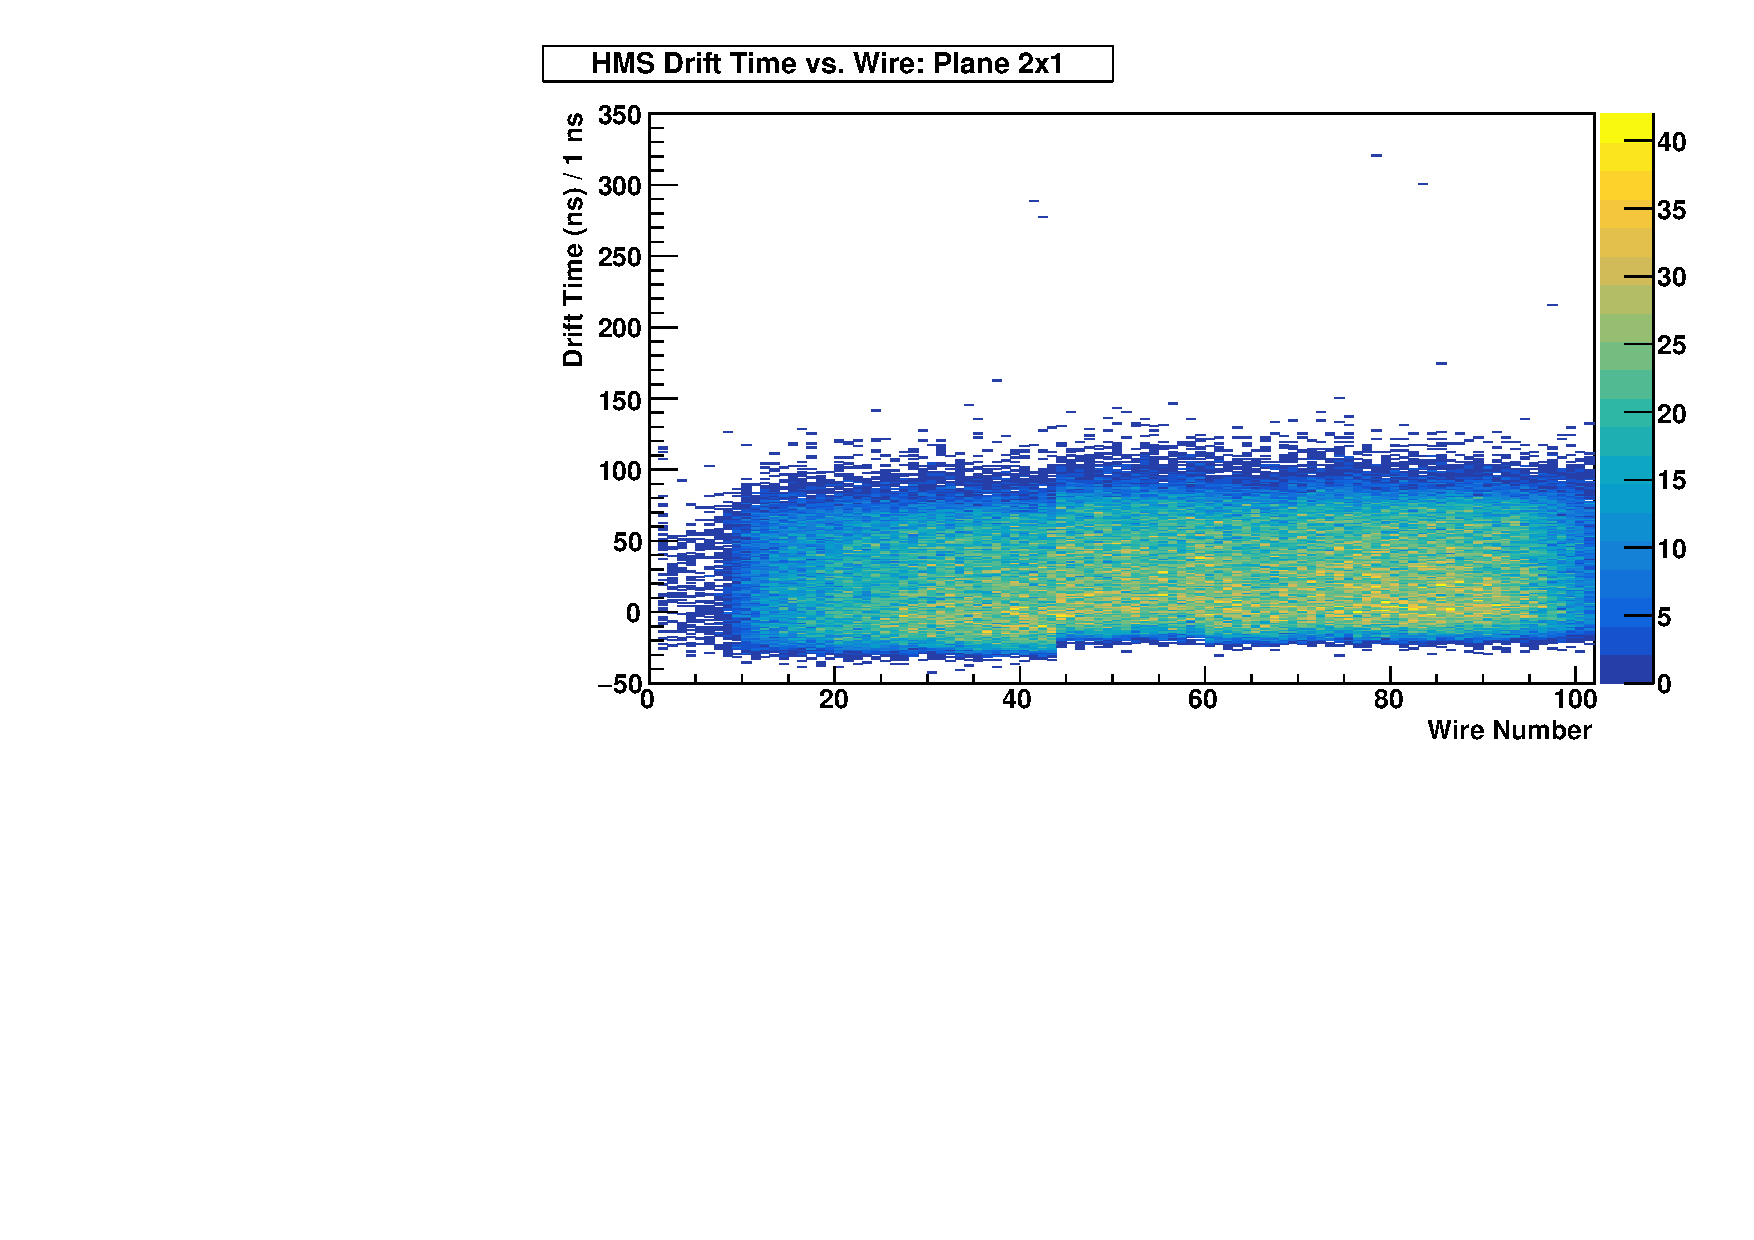
\includegraphics[width=\textwidth]{chap4/uncorrected_drift_times_2x1_TH2.pdf}
        \caption{Uncorrected drift times.}
        \label{fig:uncorrected_drift_th2}
    \end{subfigure}
    \vspace{0.1cm}
    \\
    \begin{subfigure}[b]{0.8\textwidth}
        \centering
        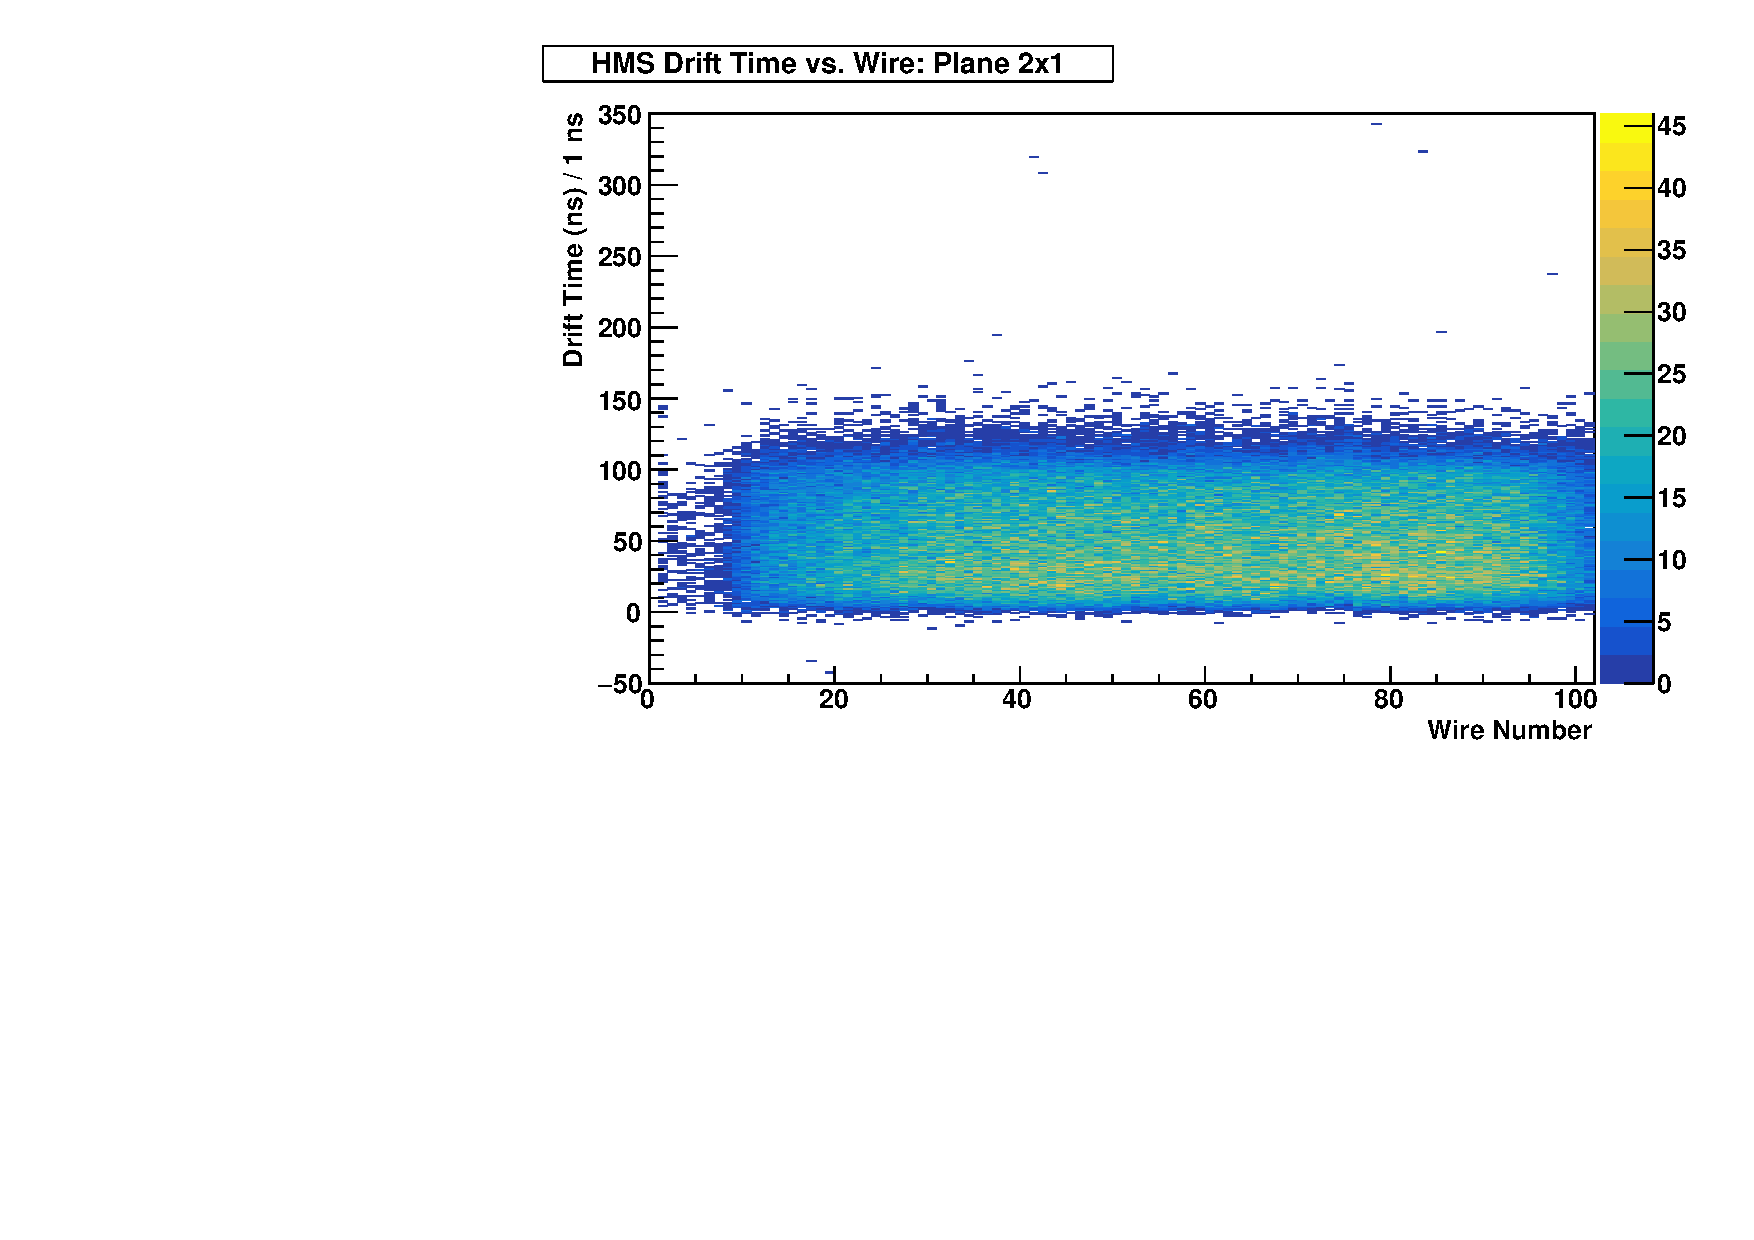
\includegraphics[width=\textwidth]{chap4/corrected_drift_times_2x1_TH2.pdf}
        \caption{Corrected drift times.}
        \label{fig:corrected_drift_th2}
    \end{subfigure}
    \caption{Two dimensional histograms of wire drift times for the HMS 2x1 plane,
             before (a) and after (b) $t_0$ correction.}
    \label{fig:drift_th2s}
\end{figure}

% TODO residuals

\subsection{Cherenkovs}

The calibration procedure for all threshold Cherenkov counters in both
spectrometers involves extracting per-PMT conversion factors $\alpha_i$ to
convert ADC pulse integrals to a number of photoelectrons.
The number of photoelectrons collected by PMT $i$ is $n_i=\alpha_iq_i$ where
$q_i$ is the pulse integral recorded for PMT $i$'s channel in the DAQ.


For the HMS Cherenkov, it is relatively straightforward to identify the single
photoelectron peak in histograms of each PMT's pedestal-subtracted pulse
integrals.
This peak can be fit with a Gaussian, the mean $\mu$ of which is the number of
\si{\pico\coulomb} generated by one photoelectron.
The conversion factor is $\alpha_i=1/\mu$.


Finding this peak for the SHMS Noble Gas Cherenkov has proved difficult, so a
second method was developed.
Events where an electron's Cherenkov radiation is focused on a single PMT are
selected by cutting on
calorimeter track-normalized energy approximately equal to 1,
track position in the PMT's quadrant at the mirror plane,
and low pulse integral in the other PMTs.
The histograms of pulse integrals for these events are again fit with a
Gaussian, from which the number of photoelectrons can be estimated to be
$N_{PE}=(\mu/\sigma)^2$.
The location of the single photoelectron peak in this histogram should then
be $\mu/N_{PE}=\mu/(\mu/\sigma)^2=\sigma^2/\mu$.
The conversion factor is $\alpha_i=\mu/\sigma^2$.


\subsection{Calorimeters}
% Plots to make for a run with good statistics
% etottracknorm
% T->Draw("H.cal.etottracknorm>>h(300,0,1.5)","H.cal.etottracknorm>0")
% shower vs preshower
% T->Draw("H.cal.etottracknorm-H.cal.eprtracknorm:H.cal.eprtracknorm>>h(100,0,1.0,120,0,1.2)","","colz")
% delta vs etottracknorm; should be vertical at 1
% T->Draw("H.gtr.dp:H.cal.etottracknorm>>h(300,0,1.5,90,-15,15)","","colz")

% Optimzation problem for calibration summarized in these slides,
% but it seems like the attenuation correction for the track y position
% is not described here.
% https://hallaweb.jlab.org/data_reduc/AnaWork2015/HMS_Calorimeter_in_HCANA.pdf

% Looking at hcana source:
% COARSE PROCESS:
%  The conversion factor is a "gain" which is the product:
%  gain = cal_{something}_cal_const[n] * cal_{something}_gain_cor[n]
%  The cal_consts are currently all 0.001. Seems silly but ok.
%
% FINE PROCESS:
%  There's a few Ycor functions in THcShower.h
%   They use parameters like cal_a_cor and a function like TMath::Exp(y/fAcor)/(1. + y*y/fBcor)
%   The parameters are in p(h)cal_geom.param.
%   Probably measured by someone like Vardan
% For reference:
% hcal_a_cor = 200.
% hcal_b_cor = 8000.
% hcal_c_cor = 64.36, 64.36
% hcal_d_cor = 1.66,  1.66
% pcal_a_cor = 106.73
% pcal_b_cor = 2.329
% pcal_c_cor = 0 0
% pcal_d_cor = 0 0

Energy deposited by particles in the calorimeters is reconstructed by
converting ADC pulse integrals recorded for each PMT to
the equivalent amount of energy converted into light collected by the PMTs.
Accurate reconstruction requires accounting for both
variations in PMT gain
and
attenuation as light propagates through the blocks.
The PMTs were matched at the hardware level to have equal output amplitudes, so
as to make the calorimeter pretrigger efficiencies as uniform as possible over
the spectrometers' acceptances.
The energy $e_i$ deposited in channel $i$ is estimated by
$e_i = \alpha_i q_i f(y)$
where
$\alpha_i$ is the channel's calibration constant,
$q_i$ is the pulse integral recorded by the DAQ,
and $f(y)$ is an attenuation correction.

\textit{hcana} first converts pulse integrals to equivalent energy with a
per-PMT conversion factor in the \texttt{CoarseProcess()} loop, and then
in the \texttt{FineProcess()} loop applies an attenuation correction
to each layer's reconstructed energy.
This correction is a function of the track's horizontal $y$ coordinate, so the
blocks in the SHMS shower array, which run roughly parallel to the $z$
coordinate, receive no attenuation correction.

The correction for blocks in HMS layers A and B, which have PMTs on both sides is:
\begin{equation}
    f_{\pm}(y) = \frac{C \pm y}{C \pm \frac{y}{D}}
\end{equation}

The correction for blocks in HMS layers C and D, which have PMTs on only one side, is:
\begin{equation}
    f(y) = \frac{e^{\frac{y}{A}}}{1 + \frac{y^2}{B}}
\end{equation}

The correction for blocks in the SHMS preshower layer is:
\begin{equation}
    f(y) = \frac{1}{1 + \left(\frac{\abs{y}}{A}\right)^B}
\end{equation}

The parameters $A$, $B$, $C$, and $D$ in the above expressions were determined
based on measurements of light transmittance made with a
spectrophotometer~\cite{Mkrtchyan_2012}.


Determining the calibration coefficients is a constrained optimization
problem~\cite{Amatuni, Vardan_cal_slides}.
Let $N$ be the number of PMTs in the calorimeter,
$q = (q_1, \cdots, q_N)^T$ their ADC pulse integrals,
$\alpha = (\alpha_1, \cdots, \alpha_N)^T$ their calibration constants,
$e_0 = E(e)$ the mean of particle energies $e$ obtained from the track reconstruction,
and $q_0 = E(q)$ the mean ADC pulse integral.
Then $e_R = \alpha^T q$ is the reconstructed particle energy.
To determine $\alpha$, the variance of the reconstructed energies with respect
to the track energies should be minimized.
That is, $E(e_R-e)^2$ should be minimized subject to the constraint
$\alpha^T q_0=e_0$.

The optimized calibration constants are
\begin{equation}
    \alpha_C = \frac{e_0 - \alpha_U^T q_0}{q_0^T Q^{-1} q_0} Q^{-1} q_0 + \alpha_U
\end{equation}
where $\alpha_U = Q^{-1}q_e$ are unconstrained calibration constants obtained
from the correlation matrix $Q=E(qq^T)$ and $q_e=E(eq)$.

\section{Tracking Algorithm}
The \textit{hcana} tracking algorithm fits a trajectory to the position of hits
recorded by the drift chamber sense wires.
As discussed in Section~\ref{sec:dc_calib}, the transverse distance between a
sense wire and a particle passing by it can be precisely estimated by
converting a reference-time-subtracted TDC time to a drift distance.
Based on a single hit, it is impossible to tell whether the particle passed by
on the left or right side of the wire.
This ambiguity is resolved by looking at nearby pairs of planes that have
identical wire orientation and spacing, but with cells displaced by half a
cell.


In each drift chamber, hits that are close ``enough'' to each other are grouped
into \textit{space points}.
The hits in each space point are fit to create \textit{stubs}, halves of a
complete track.
Stubs in both chambers are paired to form candidate tracks that are saved for
further cleaning if the paired stubs are collinear ``enough.''


In the event that multiple track candidates are found for an event, two options
for selecting the best track (referred to as the \textit{golden track}) exist.
The simplest method selects the track with the lowest $\chi^2$ value.
The other method, referred to as \textit{pruning}, involves a series of quality
assurance tests that reject suboptimal tracks.
If none of the tracks pass all the tests, this method defaults to selecting the
track with the lowest $\chi^2$.

\input{chap4/reconstruction}
\input{chap4/pid}
\section{Proton Absorption}

Because protons are strongly interacting particles, they may undergo a nuclear
reaction as they pass through the SHMS before forming an SHMS 3/4 trigger.
The corresponding electron in the HMS will have formed an HMS 3/4 trigger, but
the ``missing'' SHMS 3/4 will lead to a missing coincidence trigger.
As result, the total coincidence yield will be underestimated by some amount.
The proton absorption $A$ is the percentage of protons that, in this manner,
fail to form a coincidence trigger.


A theoretical estimate of the absorption can be obtained by considering the
proton's mean free path in the materials along its path through the SHMS.
Suppose a material is made up of components with atomic weights $A_i$, mass
density $\rho_i$, and total cross section $\sigma_{tot,i}$.
The nuclear collision length is
$\lambda_{T} = \sum_i A_i / (N_A \rho_i \sigma_{tot_i})$.
The nuclear interaction length $\lambda_{I}$ is similarly defined, subtracting
the elastic and quasielastic cross sections from $\sigma_{tot,i}$.
Because the elastic cross section is peaked in the forward direction, and will
thus remove few protons from the spectrometer's acceptance, we use the average
$\bar\lambda$ of $\lambda_T$ and $\lambda_I$ as our estimate of the mean free
path.
Our estimate of the absorption is $A=1-e^{-\sum_i X_i/\bar\lambda_i}$ where
$X_i$ is the thickness of each material in the proton's path.
Table~\ref{tab:shms_materials} lists the properties of relevant materials in
the SHMS.
Based on this table, we estimate the absorption to be $A=8.56\%$.


\vfill
% Note: in the multirow calls, the first argument is the height in lines I
% want the "system" name to span, not the number of rows in that section of
% the table.
\begin{table}[h]
    \centering
    \caption{Summary of materials in the SHMS that contribute to proton absorption.}
    \label{tab:shms_materials}
    \resizebox{1.0\textwidth}{!}{
        \begin{tabular}[t]{| l | l | l | r | r | r | r | r | r | r | r |}

            \hline
            System
            & Component                                       & Material & \thead{Thickness \\ (\si{cm})} & \thead{Density \\ (\si{\g\per\cubic\cm})} & \thead{X \\ (\si{\g\per\square\cm})} & \thead{$\lambda_T^{ a}$ \\ (\si{\g\per\square\cm})} & \thead{$\lambda_I^{ a}$ \\ (\si{\g\per\square\cm})} & \thead{$\bar{\lambda}$ \\ (\si{\g\per\square\cm})} & \thead{$X/\bar{\lambda}$ \\ ($10^-3$)}\\ \hline
            \hline

            \hline
            \multirow{6}{*}{\makecell[ml]{Target and \\ Magnets}}
            & LH2                                             & LH2                                   & 5.00                           & 0.07                                      & 0.35                                 & 42.80                                          & 52.00                                          & 47.40                                              & 7.38\\ \cline{2-10}
            & \makecell{Scattering chamber \\ exit window}    & Al                                    & 0.01                           & 2.7                                       & 0.03429                              & 69.70                                          & 107.20                                         & 88.45                                              & 0.39\\ \cline{2-10}
            & Air                                             & Air                                   & 30.00                          & 0.001                                     & 0.03675                              & 61.30                                          & 90.10                                          & 75.70                                              & 0.49\\ \cline{2-10}
            & HB entrance                                     & Al                                    & 0.03                           & 2.7                                       & 0.06858                              & 69.70                                          & 107.20                                         & 88.45                                              & 0.78\\ \cline{2-10}
            & Dipole exit                                     & Al                                    & 0.05                           & 2.7                                       & 0.13716                              & 69.70                                          & 107.20                                         & 88.45                                              & 1.55\\ \hline

            \hline
            \multirow{7}{*}{\makecell[ml]{Noble Gas \\ Cherenkov}}
            & \makecell{Entrance \\ window}                   & Tedlar                                & 0.01                           & 1.3                                       & 0.0066                               & 61.70                                          & 90.30                                          & 76.00                                              & 0.087\\ \cline{2-10}
            & Gas                                             & \makecell{\ch{CO2} \\ \SI{1.0}{\atm}} & 200.00                         & 0.002                                     & 0.396                                & 60.70                                          & 88.90                                          & 74.80                                              & 5.29\\ \cline{2-10}
            & Mirror                                          & \ch{SiO2}                             & 0.30                           & 2.2                                       & 0.66                                 & 65.20                                          & 97.80                                          & 81.50                                              & 8.10\\ \cline{2-10}
            & Mirror support                                  & Rohacell                              & 1.80                           & 0.11                                      & 0.198                                & -                                              & -                                              & 70.00                                              & 2.83\\ \cline{2-10}
            & Exit window                                     & Tedlar                                & 0.01                           & 1.3                                       & 0.0066                               & 61.70                                          & 90.30                                          & 76.00                                              & 0.087\\ \hline

            \hline
            \multirow{8}{*}{\makecell[ml]{Drift \\ Chambers}}
            & Entrance window                                 & Mylar                                 & 0.00254                        & 1.39                                      & 0.00353                              & 58.90                                          & 84.90                                          & 71.90                                              & 0.049\\ \cline{2-10}
            & Gas                                             & \makecell{50/50 \\ Ethane/Ar}         & 3.81                           & 0.002                                     & 0.00587                              & 68.60                                          & 101.00                                         & 84.80                                              & 0.069\\ \cline{2-10}
            & Field wire${^ b}$                               & W                                     & 0.00483                        & 2.7                                       & 0.01303                              & 69.80                                          & 108.00                                         & 88.90                                              & 0.147\\ \cline{2-10}
            & Sense wire${^ b}$                               & Be/Cu                                 & 0.00030                        & 19.3                                      & 0.00582                              & 110.00                                         & 185.00                                         & 147.50                                             & 0.040\\ \cline{2-10}
            & \makecell{Kapton in wire \\ and cathode planes} & Kapton                                & 0.18                           & 1.42                                      & 0.25248                              & 59.20                                          & 85.50                                          & 72.35                                              & 3.49\\ \cline{2-10}
            & Exit window                                     & Mylar                                 & 0.00254                        & 1.39                                      & 0.00353                              & 58.90                                          & 84.90                                          & 71.90                                              & 0.049\\ \hline

            \hline
            \multirow{2}{*}{\makecell[ml]{Hodoscope}}
            & \makecell{Scintilator \\ plane (x2.25)}         & PVT                                   & 1.13                           & 1.032                                     & 1.16100                              & 57.30                                          & 81.30                                          & 69.30                                              & 16.8\\ \hline

            \hline
            \multirow{5}{*}{\makecell[ml]{Heavy Gas \\ Cherenkov}}
            & Entrance window                                 & Al                                    & 0.10                           & 2.7                                       & 0.27                                 & 69.70                                          & 107.20                                         & 88.45                                              & 3.05\\ \cline{2-10}
            & Gas                                             & \makecell{\ch{CO2} \\ \SI{1.0}{\atm}} & 104.44                         & 0.002                                     & 0.20679                              & 60.70                                          & 88.90                                          & 74.80                                              & 2.76\\ \cline{2-10}
            & Mirror                                          & \ch{SiO2}                             & 0.30                           & 2.2                                       & 0.66                                 & 65.20                                          & 97.80                                          & 81.50                                              & 8.10\\ \cline{2-10}
            & Exit window                                     & Al                                    & 0.10                           & 2.7                                       & 0.27                                 & 69.70                                          & 107.20                                         & 88.45                                              & 3.05\\ \hline

            \hline
            \multirow{4}{*}{\makecell[ml]{Aerogel \\ Cherenkov}}
            & Entrance window                                 & Al                                    & 0.13                           & 2.699                                     & 0.35086                              & 69.70                                          & 107.20                                         & 88.45                                              & 3.97\\ \cline{2-10}
            & Aerogel                                         & Aeorogel                              & 9.00                           & 0.143                                     & 1.28571                              & 65.00                                          & 97.30                                          & 81.15                                              & 15.8\\ \cline{2-10}
            & Air                                             & Air                                   & 17.10                          & 0.001                                     & 0.02103                              & 61.30                                          & 90.10                                          & 75.70                                              & 0.28\\ \cline{2-10}
            & Exit window                                     & Al                                    & 0.16                           & 2.7                                       & 0.43200                              & 69.70                                          & 107.20                                         & 88.45                                              & 4.88\\ \hline
            \hline

            \hline
            \multirow{1}{*}{\makecell[ml]{Total}}
            &                                                 &                                       &                                &                                           &                                      &                                                &                                                &                                                    & 89.5\\ \hline

            \multicolumn{10}{l}{\multirow{1}{\linewidth}{\makecell[tl]{$^{a }$Nuclear
            interaction and collision lengths taken from
            PDG~\cite{pdg_material_properties}.}}} \\
            \multicolumn{10}{l}{\multirow{2}{\linewidth}{\makecell[tl]{$^{b }$The
            thicknesses of the wires are ``effective'' thicknesses, determined
            by the wire radii and cell spacings described \\ in
            subsection~\ref{subsection:drift_chambers}. This effective thickness
            of a single wire plane is the average thickness of a wire with
            radius r \\ repeated in a lattice of cell width w, seen by a particle whose position in the
            $XY$ plane is random. This effective \\ thickness is $\pi r^2/w$. \\}}}
        \end{tabular}
    } % resizebox
\end{table}
\vfill
\clearpage

\begin{figure}[!h]
    \centering
    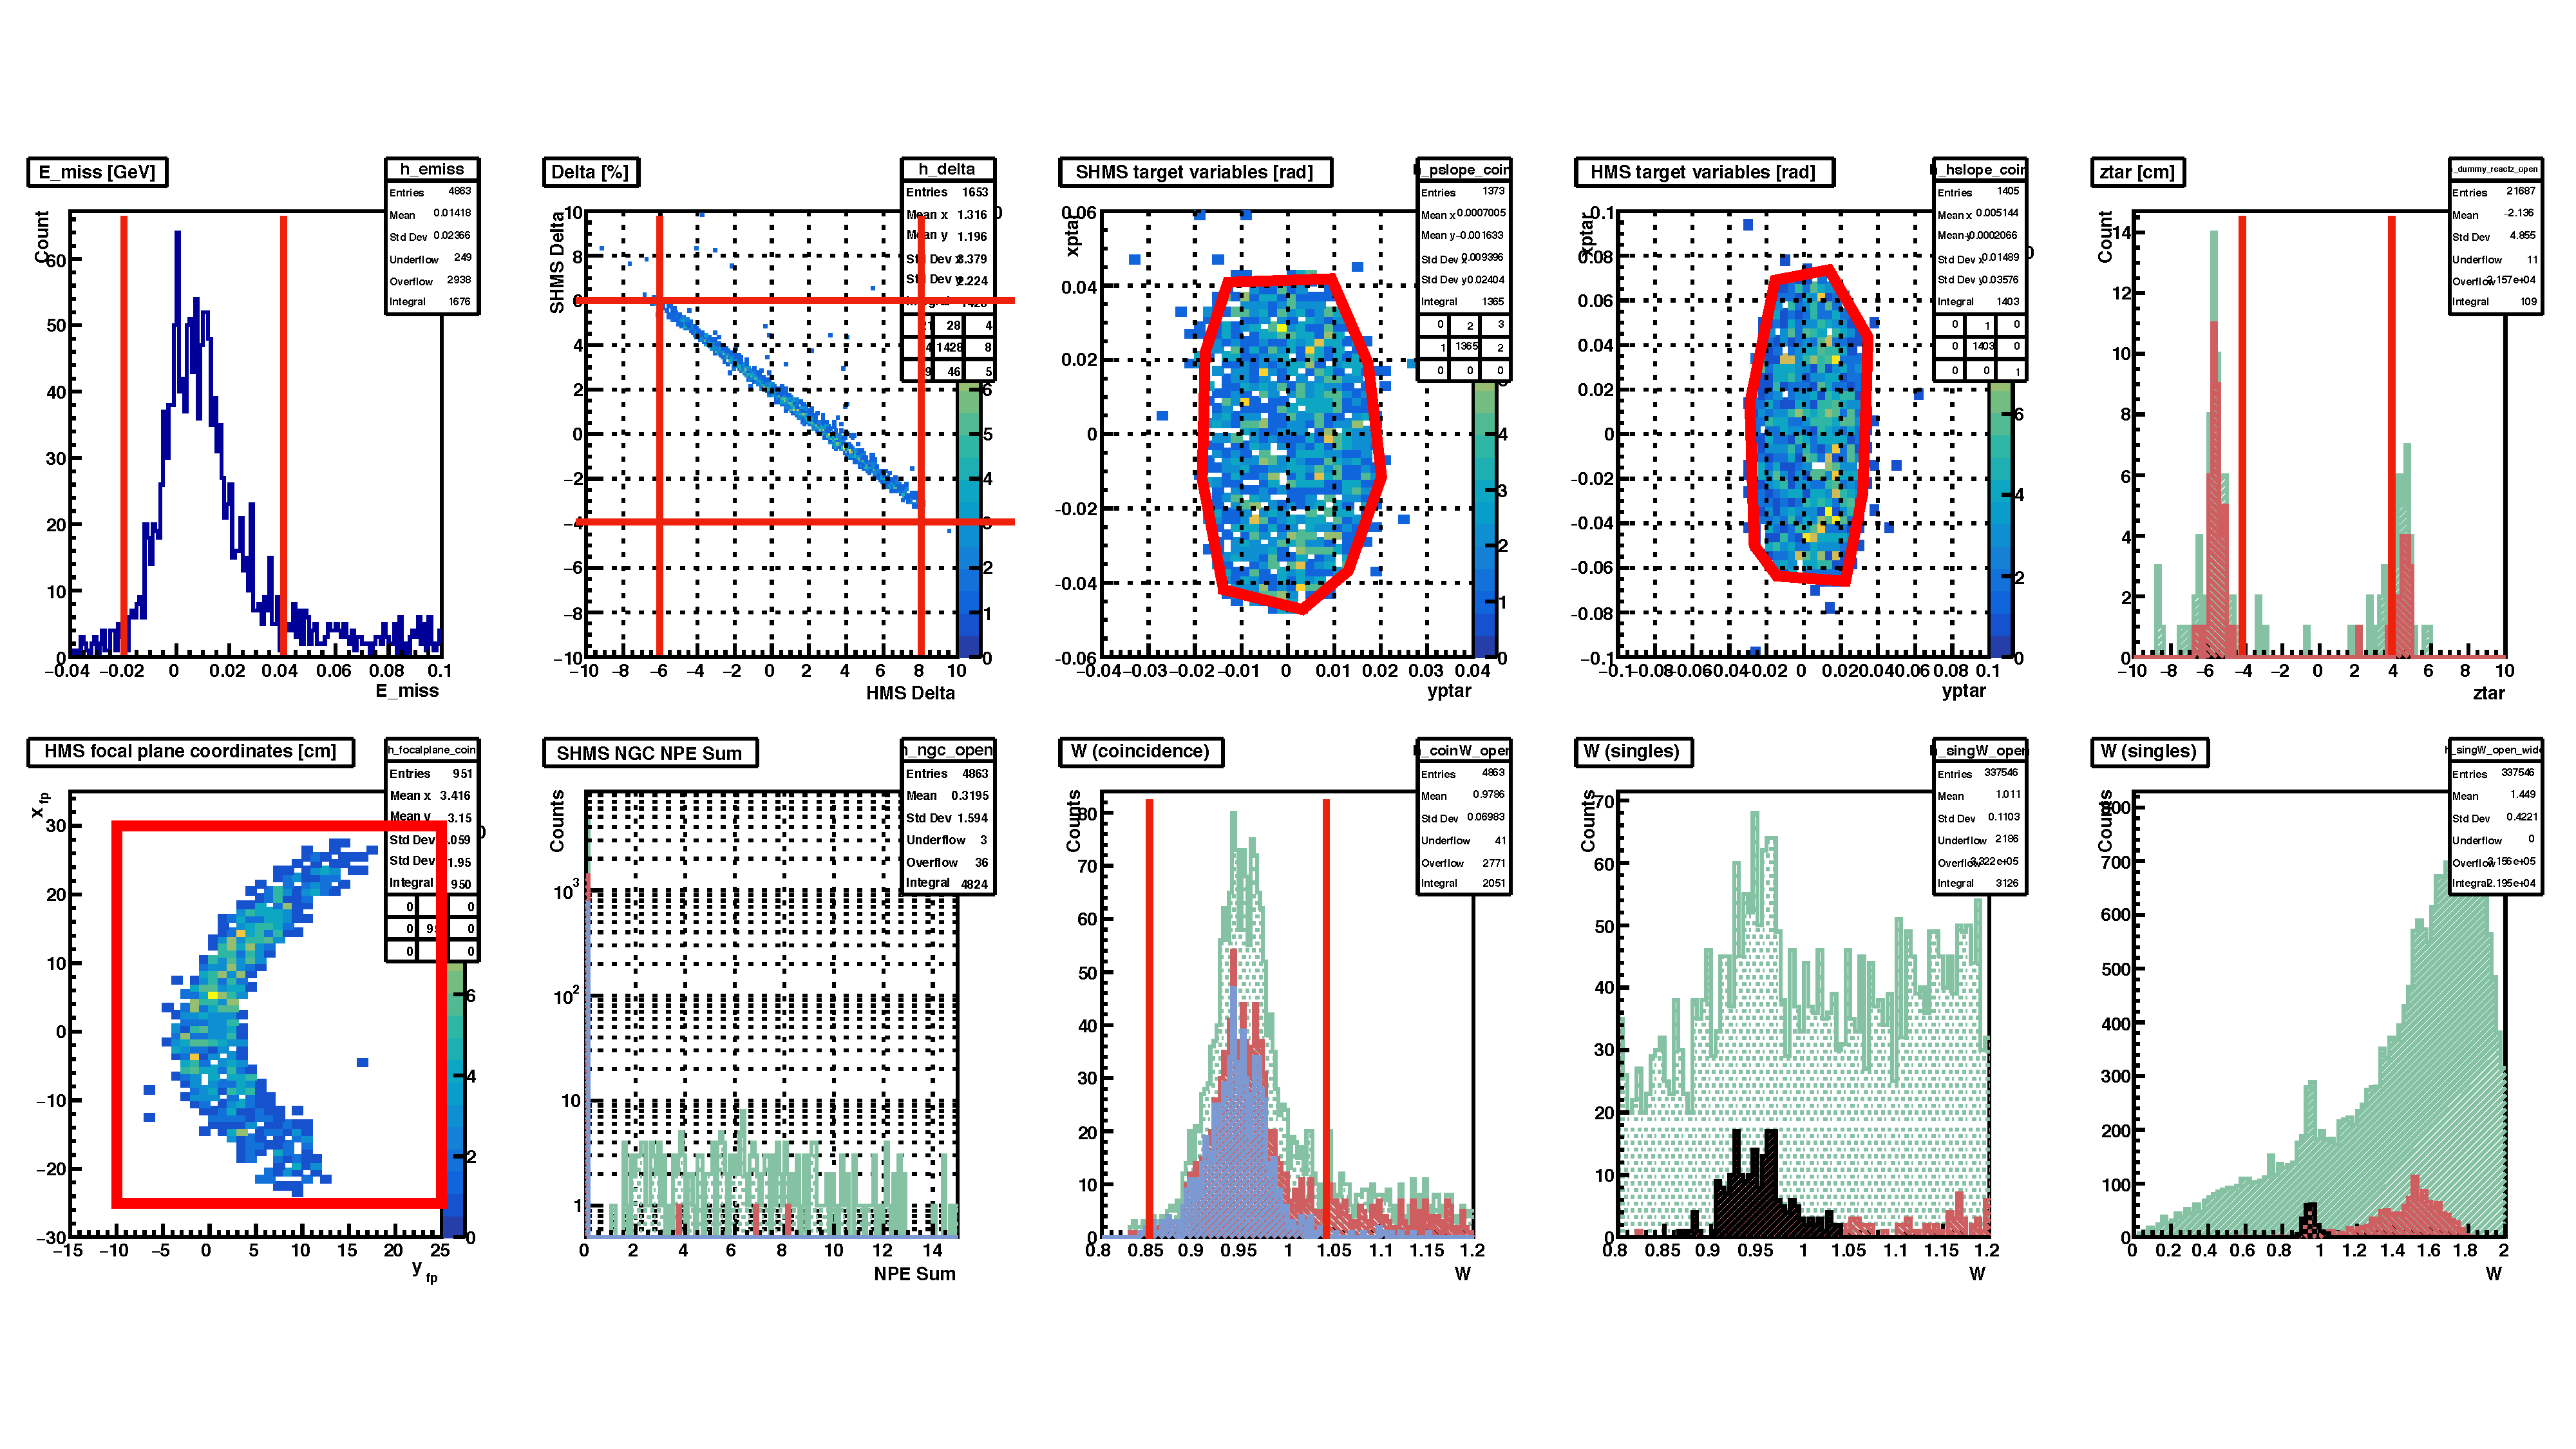
\includegraphics[width=1.0\textwidth]{chap4/proton_absorption_plots.pdf}
    \caption{Histograms of the quantities used to guide the selection of cuts
             for selecting H(e,e'p) events to estimate proton absorption.
             The red lines and contours indicate the cuts used.}
    \label{fig:proton_absorption_plots}
\end{figure}

Using the charge-normalized yields, $Y_{coin}$ and $Y_{sing}$, from coincidence
HMS singles H(e,e'p) runs, we can measure the proton absorption
$A=1-Y_{coin}/Y_{sing}$.
With a tight cut on spectrometer acceptance and invariant mass $W$ and
correcting for detector efficiencies and deadtime, $Y_{sing}$ should be an
accurate count of all electrons that participated in elastic scattering.
In contrast, $Y_{coin}$, even with the same cuts and corrections, will have
underestimated the ``true'' yield; some portion of the electrons detected in the
HMS will have corresponding protons that did not form a 3/4 trigger in the SHMS
because they were absorbed.
Using our $Q^2 = \SI{11.5}{\giga\electronvolt}$ runs and the cuts listed in
Table~\ref{tab:proton_absorption_cuts}, we estimate a proton absorption of $A=8.83 \pm 0.69 \%$.
The uncertainty quoted here is only statistical.

\begin{table}[h]
    \centering
    \caption{List of cuts used in proton absorption estimate.}
    \label{tab:proton_absorption_cuts}
    \resizebox{1.0\textwidth}{!}{
        \begin{tabular}[t]{| l | l | l | r | r | r | r | r | r | r | r |}
            \hline
            Variables              &  Cut \\ \hline
            \hline
            HMS PID                &  H.cer.npeSum>1 \&\& 0.90 < H.cal.etottracknorm \&\& H.cal.etottracknorm < 1.10 \\ \hline
            % ppidcut              &  P.ngcer.npeSum == 0 \\ \hline
            $E_{miss}$             &  -0.02 < P.kin.secondary.emiss \&\& P.kin.secondary.emiss<0.04 \\ \hline
            % pdeltacut            &  -4.0 < P.gtr.dp \&\& P.gtr.dp < 6.0 \\ \hline
            $\delta_{HMS}$         &  -6.0 < H.gtr.dp \&\& H.gtr.dp < 8.0 \\ \hline
            $x'_{tar}$,$y'_{tar}$  &  Graphical cut on HMS xptar and yptar shown in Figure~\ref{fig:proton_absorption_plots} \\ \hline
            % pslope               &  Graphical cut on SHMS xptar and yptar \\ \hline
            $z_{tar}$              &  abs(H.react.z)<3 \\ \hline
            $y_{tar}$              &  abs(H.gtr.y)<2 \\ \hline
            $x_{fp}$               &  -25<H.dc.x[0] \&\& H.dc.x[0]<30 \\ \hline
            $y_{fp}$               &  -10<H.dc.y[0] \&\& H.dc.y[0]<25 \\ \hline
            $W$                    &  0.85 < H.kin.W \&\& H.kin.W < 1.04 \\ \hline
        \end{tabular}
    } % resizebox
\end{table}

% TODO: list the method for choosing cuts
These cuts were selected by an iterative process of plotting a sequence of
histograms, each of which is plotted with a cut determined by the preceding
histograms in the sequence.
The relevant histograms are shown in Figure~\ref{fig:proton_absorption_plots}.
The process can be summarized as follows:
\begin{enumerate}
    \item Plot $E_{miss}$ for H(e,e'p) data using HMS Cherenkov and calorimeter cuts to select
        electrons. Select a cut around the peak of this distribution.
    \item Plot SHMS and HMS delta for H(e,e'p) data using that $E_{miss}$ cut and the HMS PID
        cuts. Select a cut on both.
    \item Plot HMS and SHMS $x'_{tar}$ vs $y'_{tar}$ for H(e,e'p) data using all prior cuts. Place
        a tight graphical cut on this distribution.
    \item Plot $z_{tar}$ and $y_{tar}$ for singles dummy data using cuts on HMS delta
        $x'_{tar}$, and $y'_{tar}$. Place cuts on $z_{tar}$ and $y_{tar}$ to
        remove events from the walls of the cell.
    \item Plot HMS $x_{fp}$ vs $y_{fp}$ for H(e,e'p) data using all prior cuts.
        Place a loose cut on this focal plane distribution.
    \item Define a subset of ``HMS-only'' cuts from the full set of cuts
        ``coincidence'' cuts selected so far.
    \item Examine the distributions of $W$ and SHMS Noble Gas Cherenkov NPE sum.
        Ensure that the HMS-only cuts are able to reproduce the $W$ distribution
        plotted using coincidence cuts. Ensure that there are not a significant
        number of pions showing up as non-zero entries in the SHMS Noble Gas
        Cherenkov NPE sum distribution.
    \item Using these HMS-only cuts, calculate the yields from coincidence and
        HMS singles H(e,e'p) data.
\end{enumerate}


\begin{figure}[!h]
    \centering
    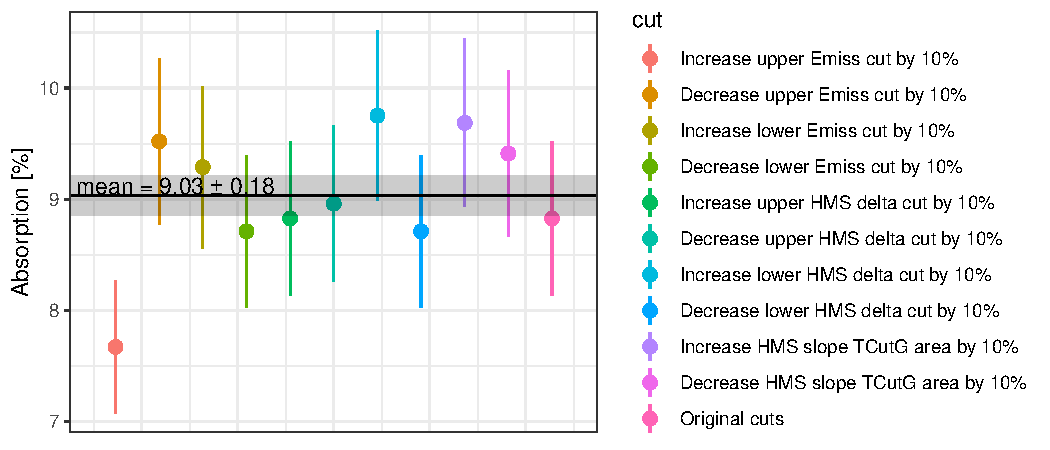
\includegraphics[width=1.0\textwidth]{chap4/proton_absorption_cut_study.pdf}
    \caption{Values of absorption estimated with 10\% variations on cuts used
             to select H(e,e'p) events.}
    \label{fig:proton_absorption_cut_study}
\end{figure}

To estimate the systematic uncertainty of this measurement, we varied the limits
of the following cuts by $\pm10\%$: $E_miss$, HMS delta, HMS xptar/yptar.
The absorption values for each of these variations are shown in
Figure~\ref{fig:proton_absorption_cut_study} along with the mean and standard
deviation of these estimates.
We use this value, $A=9.03\pm0.71\%$ as our final estimate of the proton
absorption, where the uncertainty is the quadrature sum of the systematic and
statistical uncertainties.
Note that the theoretical estimate of absorption is within the uncertainty in
this measurement.

% TODO: list runs
% TODO: include a caveat about our poor statistics and a suggestion that this
%       measurement be duplicated in a future experiment?
% TODO: include reference to Carlos's HMS measurement
% TODO: discuss momentum (in)dependence of cross sections

\section{Efficiency}
In general, the efficiency of a given detector system is estimated by using
information from other systems to select a set of ``clean'' events that can
reasonably be expected to produce a signal in that particular system.
Let $N^{should}$ be the number of events selected by a cut $C^{should}$ that
should show a signal in detector $D$, and $N^{did}$ be the subset of those
events that pass a cut $C^{did} = C^{should} \land C^{D}$,
where $C^{D}$ is an additional cut on information from the detector
$D$ under consideration and $\land$ represents the logical operation
\textit{and}.
Then the efficiency of $D$ is $\epsilon^D = N^{did}/N^{should}$.

\subsection{HMS Calorimeter} \label{sec:hcal_eff}
A set of electrons that should have normalized track energy deposition
approximately equal to one are selected using the cuts in
Table~\ref{tab:hcal_cuts}.

\begin{table}[h]
    \centering
    \caption{List of cuts used to estimate HMS Calorimeter efficiency.}
    \label{tab:hcal_cuts}
    \begin{tabular}[t]{| c | l | l |}
        \hline
                   &  Variables              &  Cut \\ \hline
        \hline
        \multirow{4}{*}{\makecell[ml]{$C^{should}$}}
        &  HMS Cherenkov NPE      &  H.cer.npeSum>0                         \\ \cline{2-3}
        &  $\delta_{HMS}$         &  -10.0 < H.gtr.dp \&\& H.gtr.dp < 10.0  \\ \cline{2-3}
        &  $\beta_{HMS}$          &  0.8 < H.gtr.beta \&\& H.gtr.beta < 1.2 \\ \cline{2-3}
        &  Good hodoscope time    &  H.hod.goodstarttime==1                 \\ \hline
        \hline
        \multirow{2}{*}{\makecell[ml]{$C^{HCal}$}}
        &  HMS Calorimeter Energy &  \makecell{0.8 < H.cal.etottracknorm \&\&  \\
                                               H.cal.etottracknorm < 1.15} \\ \hline
    \end{tabular}
\end{table}

Events are divided into $\delta$ bins of width 5 and efficiencies
$\epsilon_i=N_i^{did}/N_i^{should}$ are calculated for each bin.
A 95\% confidence interval for each bin's estimated efficiency is obtained
using the Clopper-Pearson method.
% TODO: This is a little unclear; sigma should be the difference between epsilon and the bounds
A weight $w_i=1/\sigma_i^2$ for each bin is assigned, where $\sigma_i$ is the
larger of differences between $\epsilon_i$ and the upper and lower CI bounds.
Then the weighted efficiency is
\begin{equation}
    \epsilon = \frac{\sum_i w_i \epsilon_i}
                    {\sum_j w_j}
\end{equation}
with uncertainty
\begin{equation}
    \sigma_\epsilon = \frac{1}{\sqrt{\sum_i w_i}}
\end{equation}

\subsection{HMS Cherenkov}
A set of electrons that should fire the Cherenkov
are selected using the cuts in
Table~\ref{tab:hcer_cuts}.
A weighted efficiency is calculated as discussed in Section~\ref{sec:hcal_eff}

\begin{table}[h]
    \centering
    \caption{List of cuts used to estimate HMS Chereknov efficiency.}
    \label{tab:hcer_cuts}
    \begin{tabular}[t]{| c | l | l |}
        \hline
                   &  Variables              &  Cut \\ \hline
        \hline
        \multirow{5}{*}{\makecell[ml]{$C^{should}$}}
        &  HMS Calorimeter Energy &  \makecell{0.8 < H.cal.etottracknorm \&\&  \\
                                               H.cal.etottracknorm < 1.15} \\ \cline{2-3}
        &  $\delta_{HMS}$         &  -10.0 < H.gtr.dp \&\& H.gtr.dp < 10.0  \\ \cline{2-3}
        &  $\beta_{HMS}$          &  0.8 < H.gtr.beta \&\& H.gtr.beta < 1.2 \\ \cline{2-3}
        &  Good hodoscope time    &  H.hod.goodstarttime==1                 \\ \hline
        \hline
        \multirow{1}{*}{\makecell[ml]{$C^{HCer}$}}
        &  HMS Cherenkov NPE      &  H.cer.npeSum>0                         \\ \hline
    \end{tabular}
\end{table}

% TODO: mirror
Discuss how we dealt with the broken mirror.

\subsection{SHMS Noble Gas Cherenkov}
The SHMS Noble Gas Cherenkov was used as a pion veto.
The SHMS central momenta used in this experiment range from
5.122 to \SI{8.505}{\giga\electronvolt}.
The pion threshold in this detector is \SI{4.65}{\giga\electronvolt} while the
the proton threshold is \SI{999999999}{\giga\electronvolt}.
A set of protons that should not fire the Cherenkov
are selected using the cuts in Table~\ref{tab:pcer_cuts}.
A weighted efficiency is calculated as discussed in Section~\ref{sec:hcal_eff}

\begin{table}[h]
    \centering
    \caption{List of cuts used to estimate SHMS Noble Gas Chereknov efficiency.}
    \label{tab:pcer_cuts}
    \begin{tabular}[t]{| c | l | l |}
        \hline
                   &  Variables              &  Cut \\ \hline
        \hline
        \multirow{3}{*}{\makecell[ml]{$C^{should}$}}
        &  $\delta_{SHMS}$        &  -10.0 < P.gtr.dp \&\& P.gtr.dp < 10.0  \\ \cline{2-3}
        &  $\beta_{SHMS}$         &  P.gtr.beta < 1.4 \\ \cline{2-3}
        &  Good hodoscope time    &  P.hod.goodstarttime==1                 \\ \hline
        \hline
        \multirow{1}{*}{\makecell[ml]{$C^{PCer}$}}
        &  SHMS Cherenkov NPE     &  P.ngcer.npeSum<0.1                     \\ \hline
    \end{tabular}
\end{table}

\subsection{Tracking}

\begin{table}[h]
    \centering
    \caption{List of cuts used to estimate HMS tracking efficiency.}
    \label{tab:htrack_cuts}
    \begin{tabular}[t]{| c | l | l |}
        \hline
                   &  Variables              &  Cut \\ \hline
        \hline
        \multirow{11}{*}{\makecell[ml]{$C^{should}$}}
        & Fiducial cut              & H.hod.goodscinhit==1 \\ \cline{2-3}
        & $\beta_{notrack}$         & \makecell{0.5 < H.hod.betanotrack \&\& \\
                                                H.hod.betanotrack < 1.4} \\ \cline{2-3}
        & Few hits in DC 1          & \makecell{(H.dc.1x1.nhit + H.dc.1u2.nhit + \\
                                                 H.dc.1u1.nhit + H.dc.1v1.nhit + \\
                                                 H.dc.1x2.nhit + H.dc.1v2.nhit) < 35} \\ \cline{2-3}
        & Few hits in DC 1          & \makecell{(H.dc.2x1.nhit + H.dc.2u2.nhit + \\
                                                 H.dc.2u1.nhit + H.dc.2v1.nhit + \\
                                                 H.dc.2x2.nhit + H.dc.2v2.nhit) < 35} \\ \cline{2-3}
        & SHMS Cherenkov NPE        & P.ngcer.npeSum<0.1 \\ \cline{2-3}
        & HMS Cherenkov NPE         & H.cer.npeSum>0 \\ \hline

        \multirow{1}{*}{\makecell[ml]{$C^{HTrack}$}}
        & At least one track found  & H.dc.ntrack>0 \\ \hline
    \end{tabular}
\end{table}

\begin{table}[h]
    \centering
    \caption{List of cuts used to estimate SHMS tracking efficiency.}
    \label{tab:htrack_cuts}
    \begin{tabular}[t]{| c | l | l |}
        \hline
                   &  Variables              &  Cut \\ \hline
        \hline
        \multirow{11}{*}{\makecell[ml]{$C^{should}$}}
        & Fiducial cut              & P.hod.goodscinhit==1 \\ \cline{2-3}
        & Good hodoscope time       & P.hod.goodstarttime==1 \\ \cline{2-3}
        & $\beta_{notrack}$         & P.hod.betanotrack < 1.2 \\ \cline{2-3}
        & Few hits in DC 1          & \makecell{(P.dc.1x1.nhit + P.dc.1u2.nhit + \\
                                                 P.dc.1u1.nhit + P.dc.1v1.nhit + \\
                                                 P.dc.1x2.nhit + P.dc.1v2.nhit) < 25} \\ \cline{2-3}
        & Few hits in DC 1          & \makecell{(P.dc.2x1.nhit + P.dc.2u2.nhit + \\
                                                 P.dc.2u1.nhit + P.dc.2v1.nhit + \\
                                                 P.dc.2x2.nhit + P.dc.2v2.nhit) < 25} \\ \cline{2-3}
        & SHMS Cherenkov NPE        & P.ngcer.npeSum<0.1 \\ \cline{2-3}
        & HMS Cherenkov NPE         & H.cer.npeSum>0 \\ \hline

        \multirow{1}{*}{\makecell[ml]{$C^{PSingleTrack}$}}
        & One track found           & P.dc.ntrack==1 \\ \hline


        \multirow{17}{*}{\makecell[ml]{$C^{PMultipleTrack}$}}
        & \makecell{More than one track \\ found} & P.dc.ntrack > 1 \\ \cline{2-3}
        & \makecell{Few hits on negative \\ side ADCs} & 
                \makecell{P.hod.1x.totNumGoodNegAdcHits<5 \&\& \\ 
                          P.hod.1y.totNumGoodNegAdcHits<5 \&\& \\
                          P.hod.2x.totNumGoodNegAdcHits<5 \&\& \\
                          P.hod.2y.totNumGoodNegAdcHits<5} \\ \cline{2-3}
        & Good focal plane time     &
                \makecell{-10 < P.hod.1x.fptime      \&\& \\
                                P.hod.1x.fptime < 50 \&\& \\
                          -10 < P.hod.1y.fptime      \&\& \\
                                P.hod.1y.fptime < 50 \&\& \\
                          -10 < P.hod.2x.fptime      \&\& \\
                                P.hod.2x.fptime < 50 \&\& \\
                          -10 < P.hod.2y.fptime      \&\& \\
                                P.hod.2y.fptime < 50} \\ \cline{2-3}
        & $\delta$                   & -15 < P.gtr.dp \&\& P.gtr.dp < 15 \\ \cline{2-3}
        & $y_{tar}$                  & -5 < P.gtr.y \&\& P.gtr.y < 5 \\ \cline{2-3}
        & $x'_{tar}$                & -0.2 < P.gtr.th \&\& P.gtr.th < 0.2 \\ \cline{2-3}
        & $y'_{tar}$                & -0.2 < P.gtr.ph \&\& P.gtr.ph < 0.2 \\ \hline
    \end{tabular}
\end{table}

\subsection{Trigger}

\subsection{Livetime} \label{sec:livetime}
When a trigger is accepted, the DAQ system is unable to accept additional
triggers for a time determined by the gate widths of front end electronics and
the time it takes for CODA to write the event to disk.
The time during which the DAQ is unable to accept another event is referred to
as deadtime.
The inverse concept, livetime, refers to the total time that the DAQ is
\textit{not} occupied by processing incoming triggers.
The total livetime $TLT$ is a correction applied to the charge normalized yield
to account for events that are missed because of this phenomenon.

% TODO: edtm logic diagram
The EDTM (see Section~\ref{sec:edtm}) pulser allows an estimate of the total
livetime in a given run.
It sends regular pulses at a low frequency (\SI{3}{\hertz} in our experiment) at the
trigger logic level in the counting house.
By comparing the number of triggers that are accepted by the DAQ to the number
of pulses that are counted by the EDTM scaler, we can estimate the total
livetime as
\begin{equation}
    TLT = \frac{N_{EDTM,accepted}}{N_{EDTM,scaler}}
\end{equation}
where $N_{EDTM,accepted}$ is the number of events with a non-zero hit in the
EDTM TDC spectrum and $N_{EDTM,scaler}$ is the total number of EDTM triggers
counted by the EDTM scaler.
% TODO: Peter Bosted's correction. I don't understand his derivation.
% Let n be accepted, N be scaler count. Then L=n/N
% Let j be the current, and jc be the "cut current"
% Let f=j/jc
% Then Peter's correction is Lnew = (L-(1-f))/f
% The assumption here is that livetime is 100% when the beam is "off"
% i.e. below the cut value (typically a couple uA) used by hcana


% TODO: trigger rate figure
Because livetime should be dependent on trigger rate and the trigger rates
vary between our kinematic settings, we calculate a per-run livetime to
correct each run's yield.
Moreover, the EDTM system was not functional when we took our first set of data
for $Q^2$ of \SI{8}{\giga\electronvolt\squared}.
To estimate the livetime for these data, we performed a linear fit of the other
kinematics' $TLT$ dependence on SHMS 3/4 trigger rate and used this fit to
estimate the livetime for the $Q^2$=\SI{8}{\giga\electronvolt\squared} runs.

% TODO: LTE vs pTRIG1 (SHMS 3/4)

The computer livetime can be estimated as
\begin{equation}
    CLT = \frac{N_{phys,accepted}-N_{EDTM,accepted}}{N_{phys,scaler}-N_{EDTM,scaler}}
\end{equation}
The computer livetime for our data is negligible because CODA was configured to
only take coincidence events, whose rates were all quite low (below
\SI{6}{\hertz}) for all our kinematics.

% TODO: computer livetime vs pTRIG6

% TODO: add refs for Eric and Dave's slides


\section{Simulation}

\section{Nuclear Transparency}

The nuclear transparency was extracted as the ratio of the experimental yield
to the simulated PWIA yield from \textit{SIMC} over the phase space volume $V$
defined by the limits
$E_m<\SI{80}{\mega\electronvolt}$ and
$\norm{\vec{p}_m}<\SI{300}{\mega\electronvolt}$ for ${}^{12}C(e,e'p)$
and
$E_m<\SI{100}{\mega\electronvolt}$ and
$\norm{\vec{p}_m}<\SI{100}{\mega\electronvolt}$ for $H(e,e'p)$.
\begin{equation}
    T(Q^2) = \frac{\int_{V} d^{3} p_{m} d E_{m} Y_{exp }(E_{m}, \vec{p}_{m})}
                  {\int_{V} d^{3} p_{m} d E_{m} Y_{PWIA}(E_{m}, \vec{p}_{m})}
\end{equation}

The nuclear transparency measured as a function of $Q^2$ for $H(e,e'p)$ is
shown in Fig~\ref{fig:lh2_transparency_results}.
This elastic scattering process has no final state interactions and should be
accurately modeled by the PWIA as implemented in \textit{SIMC}.
The ratio $T$ should thus be equal to one for each point, and these
measurements are consistent with $T=1$ well within the statistical and
systematic uncertainty.
This indicates that the Monte Carlo simulation in \textit{SIMC} accurately
models the scattering process and that both the spectrometers and
\textit{hcana} are accurately reconstructing physics quantities.

% TODO: replace this with a pdf
\begin{figure}[!h]
    \centering
    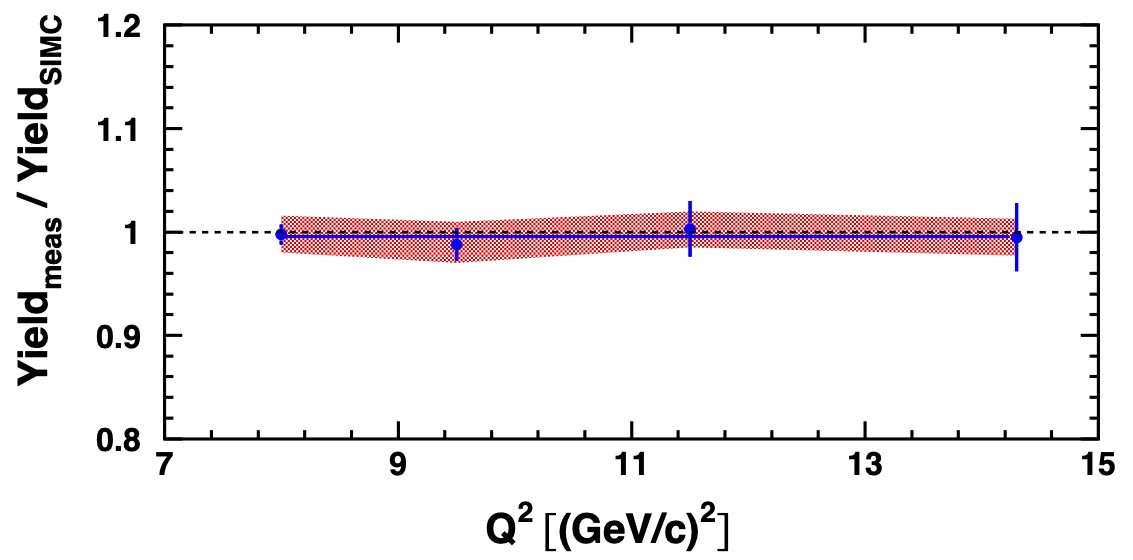
\includegraphics[width=0.8\textwidth]{chap5/lh2_results.png}
    \caption{
            Nuclear transparency for ${}^{1}H(e,e'p)$ as a function of
            momentum transfer.
            The error bars represent statistical uncertainty and the
            shaded band represents the 4.0\% systematic uncertainty.
            }
    \label{fig:lh2_transparency_results}
\end{figure}

The nuclear transparency measured as a function of $Q^2$ for ${}^{12}C(e,e'p)$
is shown in Fig~\ref{fig:lh2_transparency_results} along with previous
measurements.
Our measurements from 8--\SI{14.2}{\giga\electronvolt\squared} are consistent
with conventional multiple scattering calculations~\cite{Pandharipande_1992}
and do not support the onset of color transparency.

\begin{figure}[!h]
    \centering
    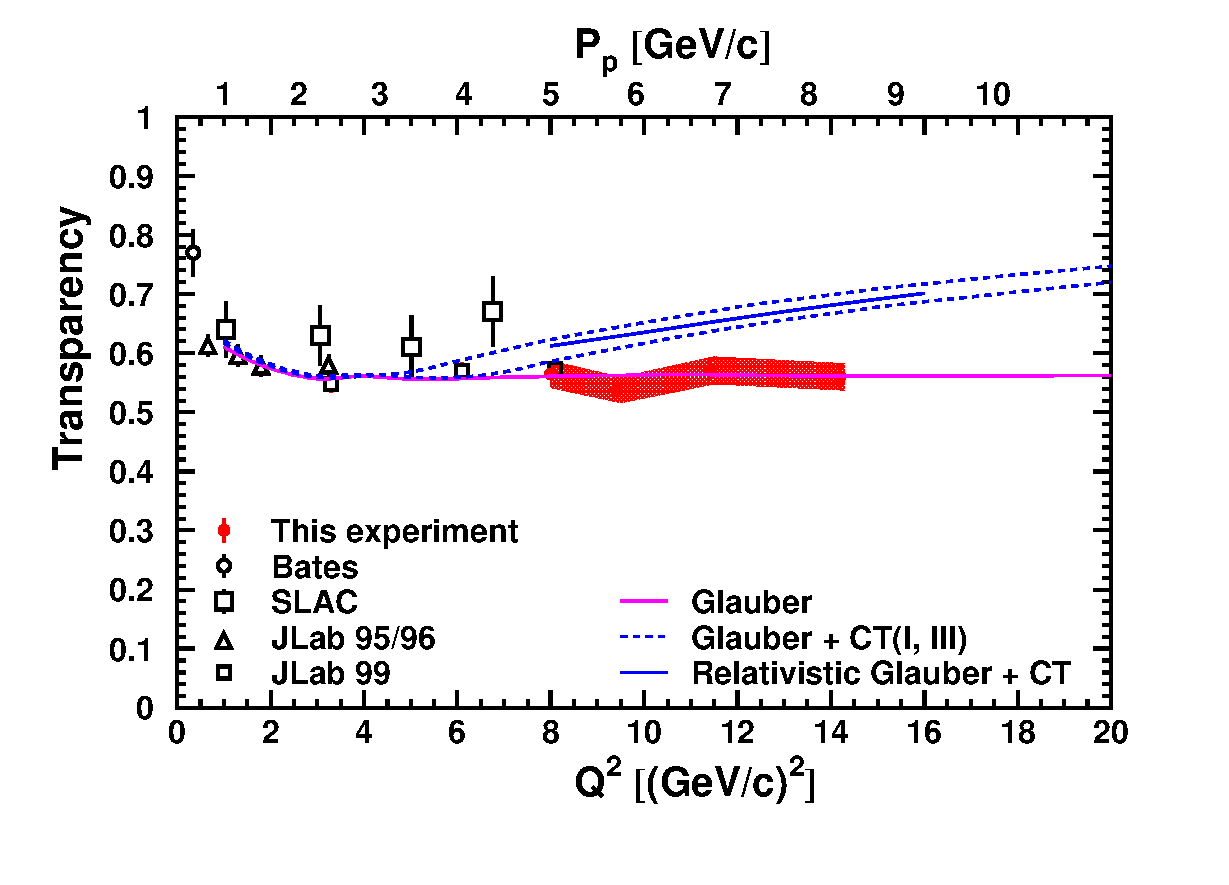
\includegraphics[width=0.8\textwidth]{chap5/c12_results.pdf}
    \caption{
            Nuclear transparency for ${}^{12}C(e,e'p)$ as a function of
            momentum transfer.
            The results of this experiment, E12-06-107, are shown in red along
            with previous measurements in open shapes.
            The error bars represent statistical uncertainty and the
            shaded band represents the 4.0\% systematic uncertainty.
            The magenta line is the prediction of a Glauber
            model that does not include CT~\cite{Pandharipande_1992}.
            The dashed lines represent predictions, for two choices of
            parameters, of a model including CT~\cite{Frankfurt_1995_PRC}.
            The solid line represents the prediction of a relativistic Glauber
            model that includes CT~\cite{Cosyn_2006}.
            }
    \label{fig:c12_transparency_results}
\end{figure}

\subsection{Systematic Uncertainty}

Table~\ref{tab:systematic_uncertainty} lists the major sources of systematic
uncertainty in our measurements of nuclear transparency.


The systematic uncertainty due to spectrometer acceptance was estimated by
taking the average of the bin-wise difference between the normalized missing
momentum spectra for data and simulation.


The uncertainty due to event selection was estimated by varying the limits of
the cuts listed in Tables~\ref{tab:lh2_cuts} and~\ref{tab:c12_cuts}
by $\pm10\%$ one at a time
and calculating the corresponding percentage change in measured transparency.
The quadrature sum of these variations was used as the systematic uncertainty.


Tracking efficiency.


Radiative corrections.


The uncertainty due to livetime and the detector efficiencies was determined
from a set of luminosity scans taken with the ${}^{12}C$ target.
The charge-normalized yield from these scans for each spectrometer was found to
be independent of the beam current within statistical uncertainties,
The average variation in the normalized yield vs beam current was recorded as the
systematic uncertainty (0.5\%).


The normalization uncertainty due to the free $ep$ cross section used in
\textit{SIMC} is 1.8\%~\cite{Bosted_1995}.
The uncertainty due to target thickness is taken from the JLab target group's
measurements. %TODO: find this citation again
The uncertainty in measured charge was estimated to be $1\%$ by varying the
minimum beam current cut used by \textit{hcana} to calculate each run's average
current.
Proton absorption.

% The total model-dependent uncertainty is 3.9\% when the uncertainty in the
% spectral function (2.8\%) and the corrections due to nucleon-nucleon
% correlations (2.7\%) are added in quadrature.

% The uncertainty in the spectral function includes the effects of the off-shell
% $\sigma_{ep}$ of 2\%, the electric and magnetic form factors of the proton
% (2\%) as previously determined\,\cite{ONeill_1995}.

\begin{table}[htb!]
    \caption{
        Systematic uncertainties in our measurements of nuclear
        transparency.
        $Q^2$-dependent uncertainties are averaged over all kinematic settings.
        The total uncertainty is the quadrature sum of the individual
        contributions.
    }
    \label{tab:systematic_uncertainty}
    \centering
    \begin{tabular}{lc}
        \hline
        \hline
        Source                            & $Q^2$-dependent uncertainty (\%) \\
        \hline
        Spectrometer acceptance           & 2.6                              \\
        Event selection                   & 1.4                              \\
        Tracking efficiency               & 0.5                              \\
        Radiative corrections             & 1.0                              \\
        Live time \& detector efficiency  & 0.5                              \\
        \hline
        \hline
        Source                            & Normalization uncertainty (\%)   \\
        \hline
        Free $ep$ cross section           & 1.8                              \\
        Target thickness                  & 0.5                              \\
        Beam charge                       & 1.0                              \\
        Proton absorption                 & 1.2                              \\
        \hline
        \hline
        Total                             & 4.0                              \\
    \end{tabular}
\end{table}


\chapter{Results}

\subsection{Missing Energy and Missing Momentum}

\begin{equation}
    E_m = \omega - T_{p'} - T_{A-1}
\end{equation}
\begin{equation}
    \vec{p}_m = \vec{p}_{p'} - \vec{q}
\end{equation}
where the kinetic energy is $T=E-m$.

\section{Nuclear Transparency}

The nuclear transparency was extracted as the ratio of the experimental yield
to the simulated PWIA yield from \textit{SIMC} over the phase space volume $V$
defined by the limits
$E_m<\SI{80}{\mega\electronvolt}$ and
$\norm{\vec{p}_m}<\SI{300}{\mega\electronvolt}$ for ${}^{12}C(e,e'p)$
and
$E_m<\SI{100}{\mega\electronvolt}$ and
$\norm{\vec{p}_m}<\SI{100}{\mega\electronvolt}$ for $H(e,e'p)$.
\begin{equation}
    T(Q^2) = \frac{\int_{V} d^{3} p_{m} d E_{m} Y_{exp }(E_{m}, \vec{p}_{m})}
                  {\int_{V} d^{3} p_{m} d E_{m} Y_{PWIA}(E_{m}, \vec{p}_{m})}
\end{equation}

The nuclear transparency measured as a function of $Q^2$ for $H(e,e'p)$ is
shown in Fig~\ref{fig:lh2_transparency_results}.
This elastic scattering process has no final state interactions and should be
accurately modeled by the PWIA as implemented in \textit{SIMC}.
The ratio $T$ should thus be equal to one for each point, and these
measurements are consistent with $T=1$ well within the statistical and
systematic uncertainty.
This indicates that the Monte Carlo simulation in \textit{SIMC} accurately
models the scattering process and that both the spectrometers and
\textit{hcana} are accurately reconstructing physics quantities.

% TODO: replace this with a pdf
\begin{figure}[!h]
    \centering
    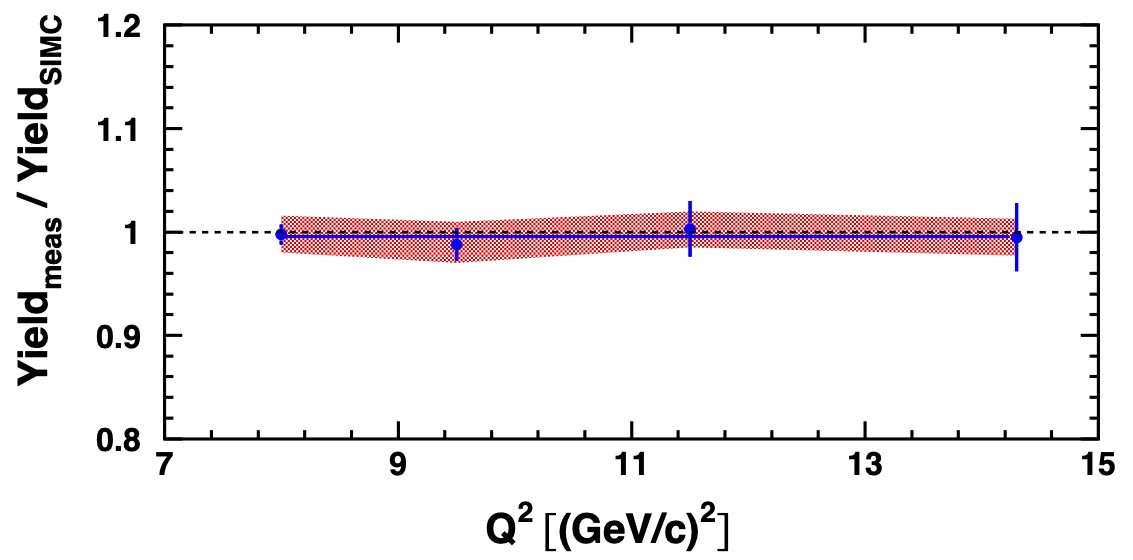
\includegraphics[width=0.8\textwidth]{chap5/lh2_results.png}
    \caption{
            Nuclear transparency for ${}^{1}H(e,e'p)$ as a function of
            momentum transfer.
            The error bars represent statistical uncertainty and the
            shaded band represents the 4.0\% systematic uncertainty.
            }
    \label{fig:lh2_transparency_results}
\end{figure}

The nuclear transparency measured as a function of $Q^2$ for ${}^{12}C(e,e'p)$
is shown in Fig~\ref{fig:lh2_transparency_results} along with previous
measurements.
Our measurements from 8--\SI{14.2}{\giga\electronvolt\squared} are consistent
with conventional multiple scattering calculations~\cite{Pandharipande_1992}
and do not support the onset of color transparency.

\begin{figure}[!h]
    \centering
    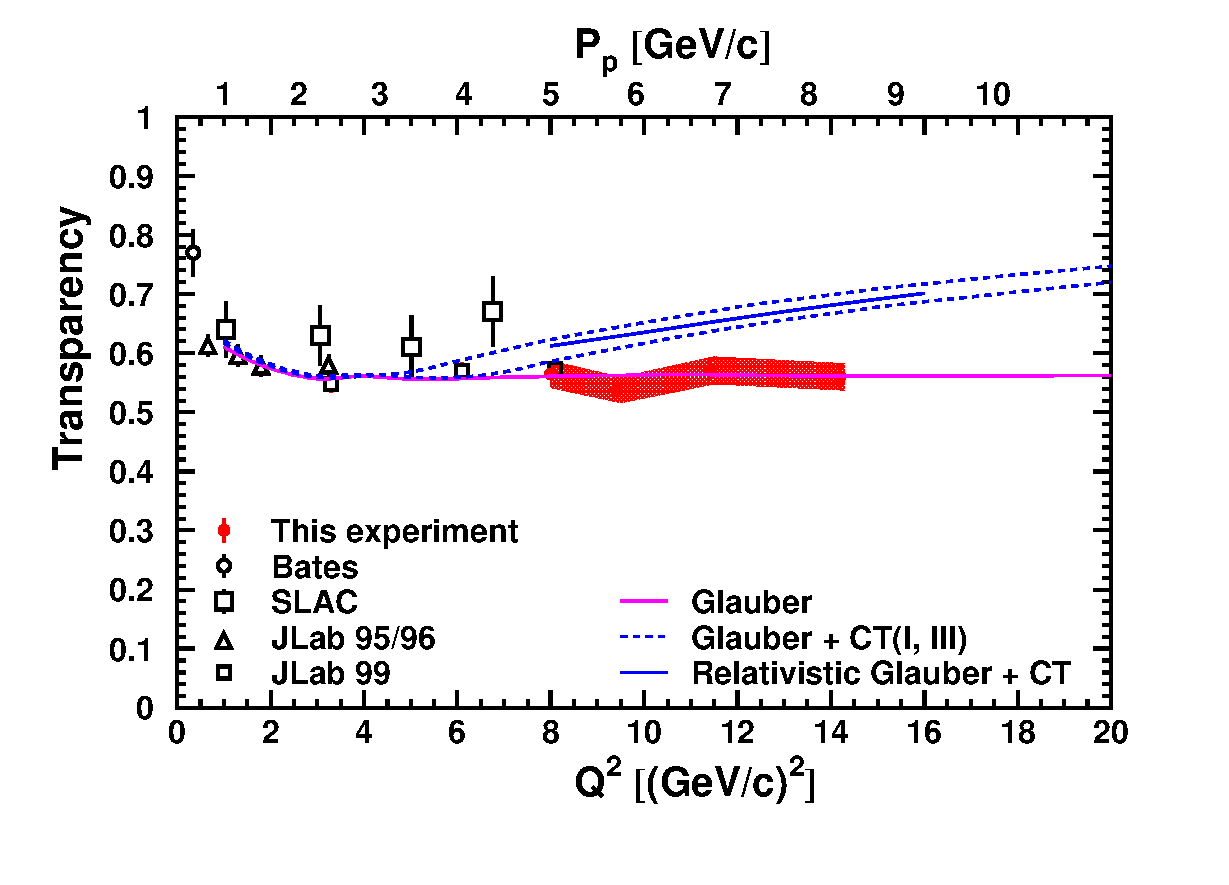
\includegraphics[width=0.8\textwidth]{chap5/c12_results.pdf}
    \caption{
            Nuclear transparency for ${}^{12}C(e,e'p)$ as a function of
            momentum transfer.
            The results of this experiment, E12-06-107, are shown in red along
            with previous measurements in open shapes.
            The error bars represent statistical uncertainty and the
            shaded band represents the 4.0\% systematic uncertainty.
            The magenta line is the prediction of a Glauber
            model that does not include CT~\cite{Pandharipande_1992}.
            The dashed lines represent predictions, for two choices of
            parameters, of a model including CT~\cite{Frankfurt_1995_PRC}.
            The solid line represents the prediction of a relativistic Glauber
            model that includes CT~\cite{Cosyn_2006}.
            }
    \label{fig:c12_transparency_results}
\end{figure}

\subsection{Systematic Uncertainty}

Table~\ref{tab:systematic_uncertainty} lists the major sources of systematic
uncertainty in our measurements of nuclear transparency.


The systematic uncertainty due to spectrometer acceptance was estimated by
taking the average of the bin-wise difference between the normalized missing
momentum spectra for data and simulation.


The uncertainty due to event selection was estimated by varying the limits of
the cuts listed in Tables~\ref{tab:lh2_cuts} and~\ref{tab:c12_cuts}
by $\pm10\%$ one at a time
and calculating the corresponding percentage change in measured transparency.
The quadrature sum of these variations was used as the systematic uncertainty.


Tracking efficiency.


Radiative corrections.


The uncertainty due to livetime and the detector efficiencies was determined
from a set of luminosity scans taken with the ${}^{12}C$ target.
The charge-normalized yield from these scans for each spectrometer was found to
be independent of the beam current within statistical uncertainties,
The average variation in the normalized yield vs beam current was recorded as the
systematic uncertainty (0.5\%).


The normalization uncertainty due to the free $ep$ cross section used in
\textit{SIMC} is 1.8\%~\cite{Bosted_1995}.
The uncertainty due to target thickness is taken from the JLab target group's
measurements. %TODO: find this citation again
The uncertainty in measured charge was estimated to be $1\%$ by varying the
minimum beam current cut used by \textit{hcana} to calculate each run's average
current.
Proton absorption.

% The total model-dependent uncertainty is 3.9\% when the uncertainty in the
% spectral function (2.8\%) and the corrections due to nucleon-nucleon
% correlations (2.7\%) are added in quadrature.

% The uncertainty in the spectral function includes the effects of the off-shell
% $\sigma_{ep}$ of 2\%, the electric and magnetic form factors of the proton
% (2\%) as previously determined\,\cite{ONeill_1995}.

\begin{table}[htb!]
    \caption{
        Systematic uncertainties in our measurements of nuclear
        transparency.
        $Q^2$-dependent uncertainties are averaged over all kinematic settings.
        The total uncertainty is the quadrature sum of the individual
        contributions.
    }
    \label{tab:systematic_uncertainty}
    \centering
    \begin{tabular}{lc}
        \hline
        \hline
        Source                            & $Q^2$-dependent uncertainty (\%) \\
        \hline
        Spectrometer acceptance           & 2.6                              \\
        Event selection                   & 1.4                              \\
        Tracking efficiency               & 0.5                              \\
        Radiative corrections             & 1.0                              \\
        Live time \& detector efficiency  & 0.5                              \\
        \hline
        \hline
        Source                            & Normalization uncertainty (\%)   \\
        \hline
        Free $ep$ cross section           & 1.8                              \\
        Target thickness                  & 0.5                              \\
        Beam charge                       & 1.0                              \\
        Proton absorption                 & 1.2                              \\
        \hline
        \hline
        Total                             & 4.0                              \\
    \end{tabular}
\end{table}


\chapter{Summary and Conclusion}
Using the upgraded 12\,\,GeV CEBAF beam at JLab, coincidence $(e,e'p)$ data
were taken with $^{1}H$ and $^{12}C$ targets for $Q^2$ values between 8 and
14.2\,(GeV/$c)^2$.
Nuclear transparencies were extracted for each kinematic point by integrating
charge-normalized yields and taking their ratio.
The transparency measured at the lowest kinematic point at
$Q^2=8.1$\,(GeV/$c)^2$ agrees with prior measurements at JLab.
The $Q^2$-dependence of the measured transparencies is consistent with
traditional Glauber multiple scattering theory and does not show an onset of
color transparency in $^{12}C(e,e'p)$ below $Q^2=14.2$\,(GeV/$c)^2$.
% Though other work has suggested that the onset may be more obvious in the
% $s$-shell than in the $p$-shell, this effect is not evident in this
% experiment's results.

As discussed in Sec~\ref{sec:ct_def}, Brodsky and de Téramond~\cite{Brodsky_2021}
use light-front holographic QCD to derive an expression for a PLCs transverse
size as a function of twist $\tau$ and $Q^2$.
Their calculations suggest that the onset of CT in ${}^{12}C(e,e'p)$ may be
higher than what can currently be probed in Hall C, perhaps not occurring
until $Q^2=\SI{20}{\giga\electronvolt\squared}$.

Using the same framework, Caplow-Munro and Miller~\cite{CaplowMunro_2021}
demonstrate that expansion effects are not sufficiently large to cause FSI in
this experiment's measurements.
The lack of a rise in transparency then suggests that a PLC was not formed,
and that the proton's electromagnetic form factor is dominated at large
momentum by the Feynman mechanism\footnote{In the Feynman mechanism, a single
quark carrying a large portion of a hadron's momentum absorbs the entire
momentum transfer $Q$~\cite{Drell_1970}.} rather than a PLC.

Experiments at JLab in the near future will include color transparency studies
in rho (Hall B) and pion (Hall C) electroproduction, and pion photoproduction
in Hall D.

\appendix
\chapter{SIMC} \label{app:simc}

% The general structure of SIMC's simulation for (quasi)elastic
% scattering is described below.
% \begin{enumerate}
%     \item Initialization
%     \begin{itemize}
%         \item Choose a reaction and final state
%         % \item Disable/enable implementation of (or correction for) raster, eloss ...
%     \end{itemize}

%     \item Event Generation
%     \begin{itemize}
%         \item Generate an event vertex based on target geometry,
%               beam width, beam raster, and beam energy
%         \item Generate $\theta_e$, $\phi_e$, $p_e$,
%                        $\theta_p$, $\phi_p$, $p_p$
%     \end{itemize}

%     \item Event Propagation
%     \begin{itemize}
%         \item Adjust event for radiative effects, Coulomb corrections, particle decays, etc.
%         \item Propagate particles through spectrometers using COSY models,
%               applying energy loss and multiple scattering in the target and
%               detectors.
%     \end{itemize}

%     \item Event Reconstruction
%     \begin{itemize}
%         \item Fit tracks in the focal plane
%         \item Reconstruct target variables $\delta$, $x'_{tar}$, $y'_{tar}$, $y_{tar}$
%     \end{itemize}

%     \item Normalization and Saving to Disk
%     \begin{itemize}
%         \item Calculate $E_m$ and $\vec{p}_m$ if simulating quasielastic scattering
%         \item Calculate per-event weight from spectral function, cross section,
%               radiative correction weight, and event generation weight.
%         \item Calculate normalization factor \textit{normfac} from luminosity,
%               phase space factors, and total number of events generated.
%         \item Save per-event physics quantities and weights in an Ntuple in a
%               PAW HBOOK.
%     \end{itemize}
% \end{enumerate}

% \textit{SIMC}'s output \texttt{.hbook} files can be converted to \texttt{.root}
% files for analysis alongside \textit{hcana} output using the utility
% \textit{h2root}.

% Good note explaining normfac
% https://hallaweb.jlab.org/12GeV/experiment/E12-07-108/Publications/Technical/Spectrometer/SIMC/simc_extra.pdf
% Gaskell/Arrington talk on simc
% https://hallaweb.jlab.org/collab/meeting/2009-winter/talks/Analysis%20Workshop%20--%20Dec%2014/simc_overview.pdf

\section{Spectral Functions}

The spectral functions used in SIMC are based on the independent particle shell
model (IPSM), which assumes nucleons occupy shells with quantum numbers $n$,
$l$, $j$, similar to the model of electron orbitals in atomic physics.
% preetty good slides
% http://indico.ictp.it/event/7641/session/21/contribution/46/material/0/0.pdf
In this model, the spectral function can be factored into a sum of per-shell
energy and momentum distributions
\begin{equation}
    S(E_m,\vec{p}_m) = \sum_i N_i \norm{\varphi_i(\vec{p})}^2 L_i(E_m)
\end{equation}
where $N_i$ is the occupation number of the $i$th shell,
$\varphi_i(\vec{p})$ is the bound state wavefunction,
and $L_i(E_m)$ is an energy profile.


% TODO: Give one of these Ls a tilde or prime to account for normalization?
The energy profile of each nuclear shell $i$ with binding energy $E_i$ is
given by a Lorentzian with finite width $\Gamma_i$ that accounts for the finite
lifetime of the one-hole state.
\begin{equation}
    L_i(E) = \frac{1}{\pi} \frac{\Gamma_i/2}{(E-E_i)^2 + \Gamma_i^2/4}
\end{equation}

The separation energy $E$ cannot be less than the minimum proton removal
energy $E_{min}=m_p + m_{A-1} - m_A$, so these profiles are cut off below
$E_min$ and normalized to ensure the spectroscopic sum rule,
Equation~\ref{eqn:spectroscopic_sum_rule}, is obeyed.
\begin{equation}
    L_i(E) =
    \begin{cases}
        L_i(E) / \int^{\infty}_{E_{min}} L_i(E) dE & \text{if $E \geq E_{min}$} \\
        0 & \text{if $E<E_{min}$}
    \end{cases}
\end{equation}


The wavefunctions $\varphi_i(\vec{p})$ are Fourier transforms of solutions
$\psi(\vec{r})$ to the Schroedinger equation with a potential given by the sum
of a
Woods-Saxon potential $-V_0 f(\vec{r})$,
Coulomb potential $V_C(r)$,
and spin-orbit coupling,
\begin{equation}
    V(\vec{r}) = - V_{0} f(r)
                 + V_{C}(r)
                 + V_{SO} \left(\frac{\hbar}{m_\pi c}\right)^{2}
                          \frac{2}{r} \frac{df}{dr}
                          \vec{l}\cdot\vec{s}
\end{equation}

The Woods-Saxon potential is characterized by
depth $V_0$,
radius $R_0=r_0(A-1)^{1/3}$, and
diffuseness $a$
parameters and a form given by a Fermi-Dirac distribution
\begin{equation}
    f(r) = \frac{1}{1+e^{\frac{r-R_0}{a}}}
\end{equation}
The Coulomb potential is that of a uniform sphere of radius
$R_c=r_c(A-1)^{1/3}$.


The model parameters were obtained from fits to the Saclay
measurements~\cite{Mougey_1976, Frullani_1984} of the ${}^{12}C$ spectral
functions.
The wavefunctions were obtained using the method described in
Ref~\cite{Giusti_1988, Giusti_1987, Blok_1991}.
% TODO: clarify: is this still the DWEEPY stuff others describe?
% TODO: table of relevant parameters?


Short range nucleon-nucleon correlations push protons to higher missing energy
and momentum than accounted for by the IPSM.
Without correcting for this, simulated yields would be artificially large.
Assuming this leads to a uniform suppression of the spectral function below the
Fermi momentum, the spectral functions can be corrected by a constant factor,
assuming one consistently works in the same volume $V_m$ of $(E_m,\vec{p}_m)$ phase
space.
Given spectral functions $S_{SRC}$,that include the effects of short range
correlations, the correction is given by
\begin{equation}
    \frac{\int_{V_m} S_{IPSM}(E_m,\vec{p}_m) dE_m d^3p_m}
         {\int_{V_m} S_{SRC} (E_m,\vec{p}_m) dE_m d^3p_m}
\end{equation}
% DD: A more realistic estimate of the SRC correction would have different
% values for the p and s-shell with the overall correction averaging to 12%

\section{Coulomb Corrections}
Coulomb distortions of the PWIA model arise from electromagnetic interactions
between the beam electron and target nucleus, modifying the momentum transfer
and incoming/outgoing momenta of the electron.


The energy required to bring an electron from infinity to a position $\vec{r}$
inside a nucleus with $Z-1$ protons is
\begin{equation}
    \Delta E(\vec{r})=f_{C}(|\vec{r}|)\left[\alpha \frac{(Z-1)}{R_{0}}\right]
\end{equation}
where
$\vec{r}=0$ is the center of the nucleus,
$\alpha$ is the fine structure constant,
and
$R_0=1.1 A^{1/3}+0.86 A^{-1/3}$ is the radius of the nucleus.


\textit{SIMC} uses the prescription described in Ref~\cite{Aste_2005}, which
takes this energy to be
\begin{equation}
    \Delta E = \frac{f(Z-1)\alpha}{R_0}
\end{equation}
where the factor $f$ is of order 1; SIMC uses $f=1.125$.


Assuming the incoming electron is not deflected, its initial momentum at the
interaction vertex becomes
\begin{equation}
    (\vec{p}_e)_v = \vec{p}_e(1 + \Delta E / p_e)
\end{equation}
This value is used to calculate the momentum transfer
\begin{equation}
    \vec{q} = (\vec{p'}_e)_v - (\vec{p}_e)_v
\end{equation}
and opposite correction is applied to the outgoing electron momentum,
\begin{equation}
    \vec{p}_e = (\vec{p'}_e)(1 - \Delta E / (p'_e)_v)
\end{equation}

% \section{Final State Interactions}
% TODO: FSI in SIMC


% \section{Pauli Blocking}
% TODO: write Pauli blocking section? I don't think we actually use it in QE simulation?
% Basic idea:
% In Fermi gas, all states below k_F are filled.
% When a pion is produced in A(e,e'pi+)n, the recoil neutron might not have
% anywhere to go!
% So occupation levels are smoothed out.
% SIMC uses Fantoni 1984 data for this.

\section{Radiative Corrections}
The method for radiative corrections in \textit{SIMC} is based on the work of
Mo and Tsai~\cite{Mo_1969}.
The full derivation by Makins et. al~\cite{Ent_2001, Makins_1994} for
coincidence elastic and quasielastic scattering done is quite length.
What follows in this section is an overview of the main results.
In brief, \textit{SIMC} calculates vertex corrections and the energy radiated
as internal and external Bremsstrahlung, modifies the simulated particles'
vertex 4-momenta accordingly, and applies a weight to the event.

\subsection{Internal Bremsstrahlung}
The cross section for scattering an electron into a solid angle $d\Omega_e$
accompanied by the emission of a single photon with momentum in the range
$d^3\omega$ is
\begin{align}
    \frac{d\sigma}{d\Omega_e d^3\omega} &=
        \left.\frac{d \sigma^{(1)}}{d \Omega_{e}}\right|_{e p}
        \frac{-\alpha}{4 \pi^{2} (\omega^{0})^2}
        \left[ \frac{k'}{\omega \cdot k'} -
                \frac{p'}{\omega \cdot p'} -
               \frac{k}{\omega \cdot k} +
               \frac{p}{\omega \cdot p}
        \right]^2 \\
     &= \left. \frac{d\sigma^{(1)}}{d\Omega_e}\right|_{ep}
         \frac{A(\hat{\omega})}{\omega^0}
\end{align}

where $\left. \frac{d\sigma^{(1)}}{d\Omega_e}\right|_{ep}$ is the single-photon
exchange $ep$ cross section,
and $A(\hat{\omega})$ is the angular distribution of single photon Bremsstrahlung.
The kinematic terms on the right hand side come from the
amplitudes given by the Feynman diagrams in Fig~\ref{fig:single_photon_brem_feynman}

\begin{figure}[!h]
    \centering
    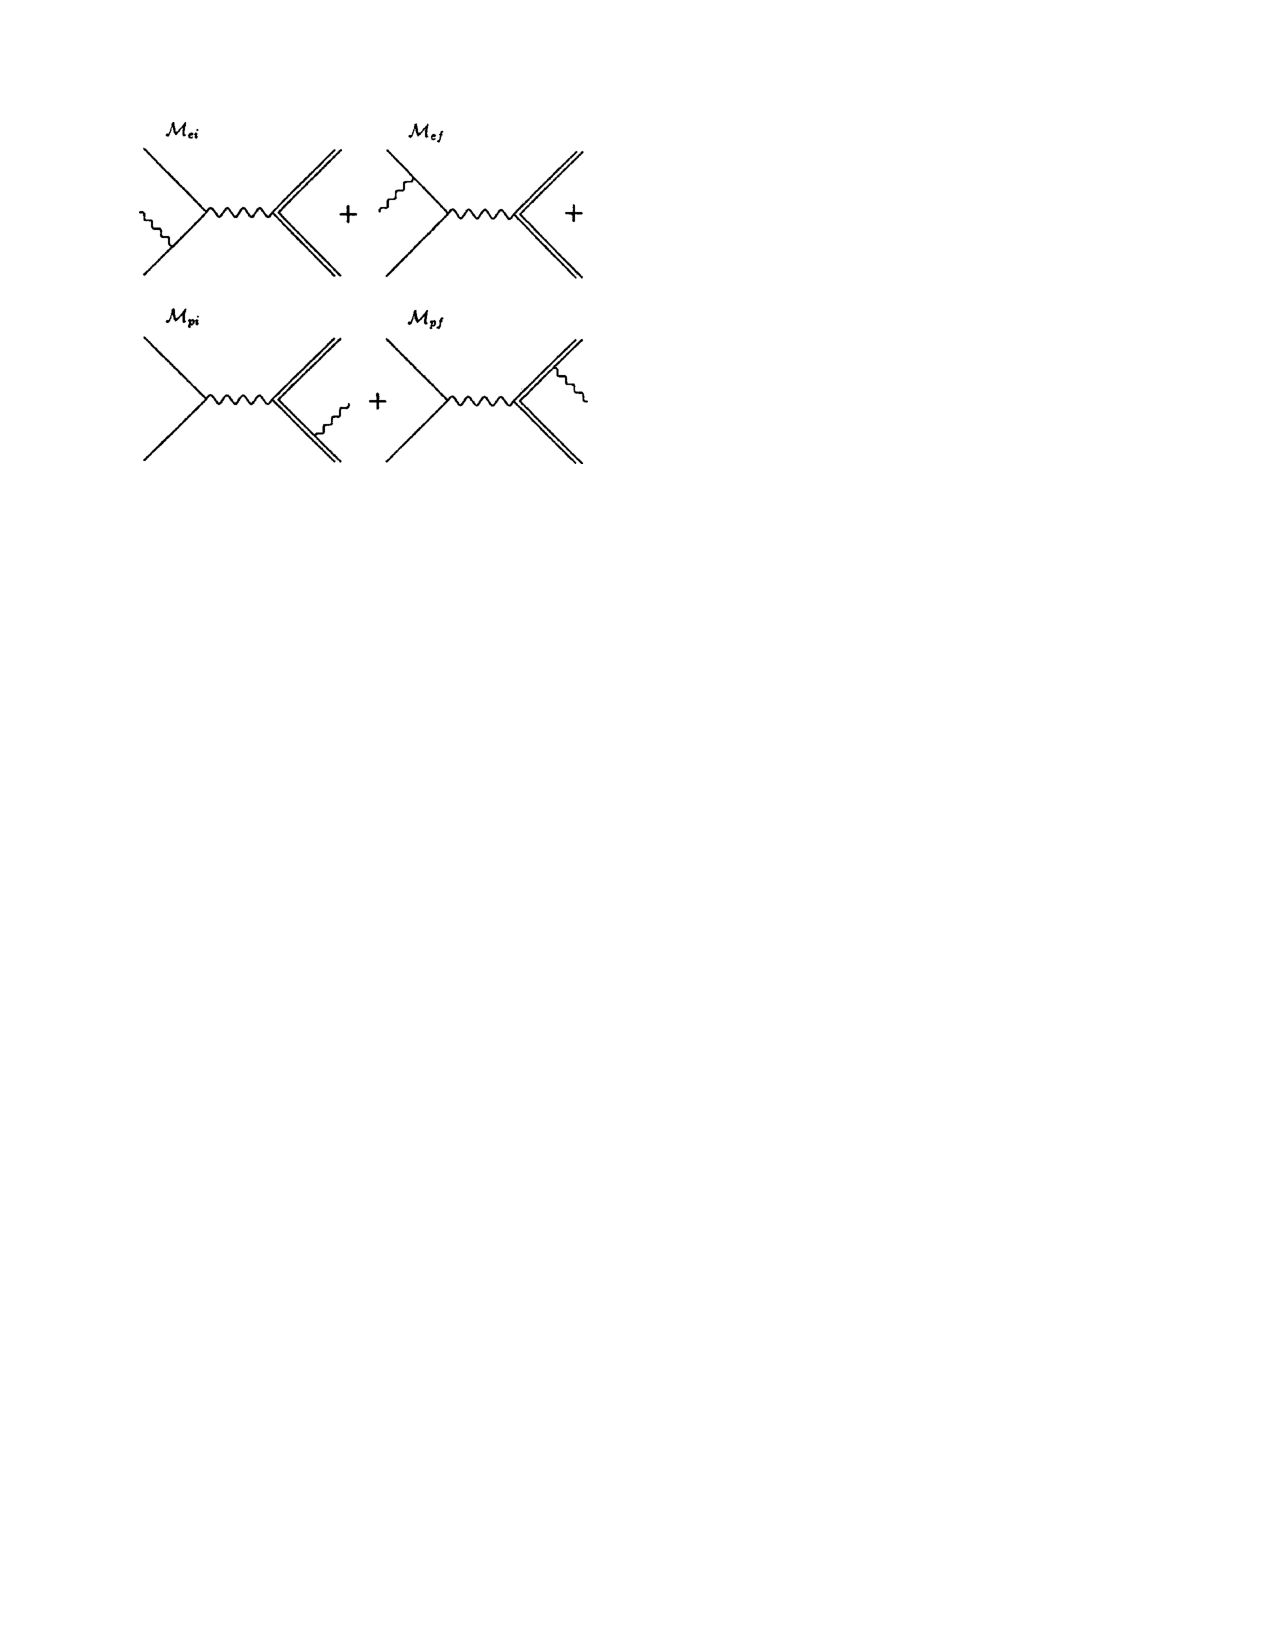
\includegraphics[width=0.7\textwidth]{chap1/single_photon_brem_feynman.pdf}
    \caption{
             Figure reproduced from Ref~\cite{Ent_2001}.
             }
    \label{fig:single_photon_brem_feynman}
\end{figure}

% TODO: remove some of this derivation stuff so we only have main results
Let
\begin{equation}
    B(p_i, p_j, \Delta E_m) = \int_0^{\Delta E_m} d^3 \omega
    \frac{1}{8\pi^2\omega^0}
    \frac{p_i \cdot p_j}{(\omega \cdot p_i)(\omega \cdot p_j)}
\end{equation}
and
\begin{equation}
    \lambda = \int d\Omega_\gamma A(\hat{\omega})
\end{equation}

Allowing the emission of multiple Bremsstrahlung photons, with a total energy
$E_{tot}$,

\begin{equation}
    \frac{d\sigma}{d\Omega_e d^3\omega} =
        \left.\frac{d \sigma^{(1)}}{d \Omega_{e}}\right|_{e p}
        (1-\sigma_{hard})
        (-\delta'_{soft}(E_{tot})
        e^{-\delta_{soft}(E_{tot})}
        F(\lambda)
\end{equation}

where $F(\lambda)=\frac{e^{-C\lambda}}{\Gamma(1+\lambda)}$ and $C$ is the
Euler-Mascheroni constant.
% TODO: clarify: is \delta'_{soft}(E) = \frac{d\delta_{soft}(E)}{dE}?


The contribution from one photon Bremsstrahlung is
\begin{equation}
    \delta_{soft}(\Delta E_m) = 2\alpha \sum_{i,j} \Theta(p_i) \Theta(p_j)
                                                   \bar{B}(p_i,p_j,\Delta E_m)
\end{equation}
where $\bar{B}(p_i,p_j,\Delta E_m)$ is $B(p_i,p_j,\Delta E_m)$ without the
infrared divergent term
$p_i$ is one of $k,k',p,p'$
and
$\Theta(p_i)$ is the sign function.

The contribution from one-loop diagrams is
\begin{equation}
    \delta_{hard} = 2\alpha
                    \left[
                        -\frac{3}{4\pi}\log\left(\frac{-q^2}{m_e^2}\right)
                        + \frac{1}{\pi}
                        - \sum_i \delta^{vp}_i(q^2)
                    \right]
\end{equation}
where
\begin{equation}
    \delta^{vp}_i = \frac{1}{3 \pi}
                        \left(
                            -\frac{5}{3} - \frac{4 m_{i}^{2}}{q^{2}} +
                            \left(1+\frac{2 m_{i}^{2}}{q^{2}}\right)
                            \sqrt{1-\frac{4 m_{i}^{2}}{q^{2}}}
                            \log \left[\frac{\sqrt{1-\frac{4 m_{i}^{2}}{q^{2}}}+1}
                                            {\sqrt{1-\frac{4 m_{i}^{2}}{q^{2}}}-1}
                                 \right]
                        \right)
\end{equation}
is the vacuum polarization correction due to flavor $i$ of leptons and light quarks of flavor $i$.

\begin{figure}[!h]
    \centering
    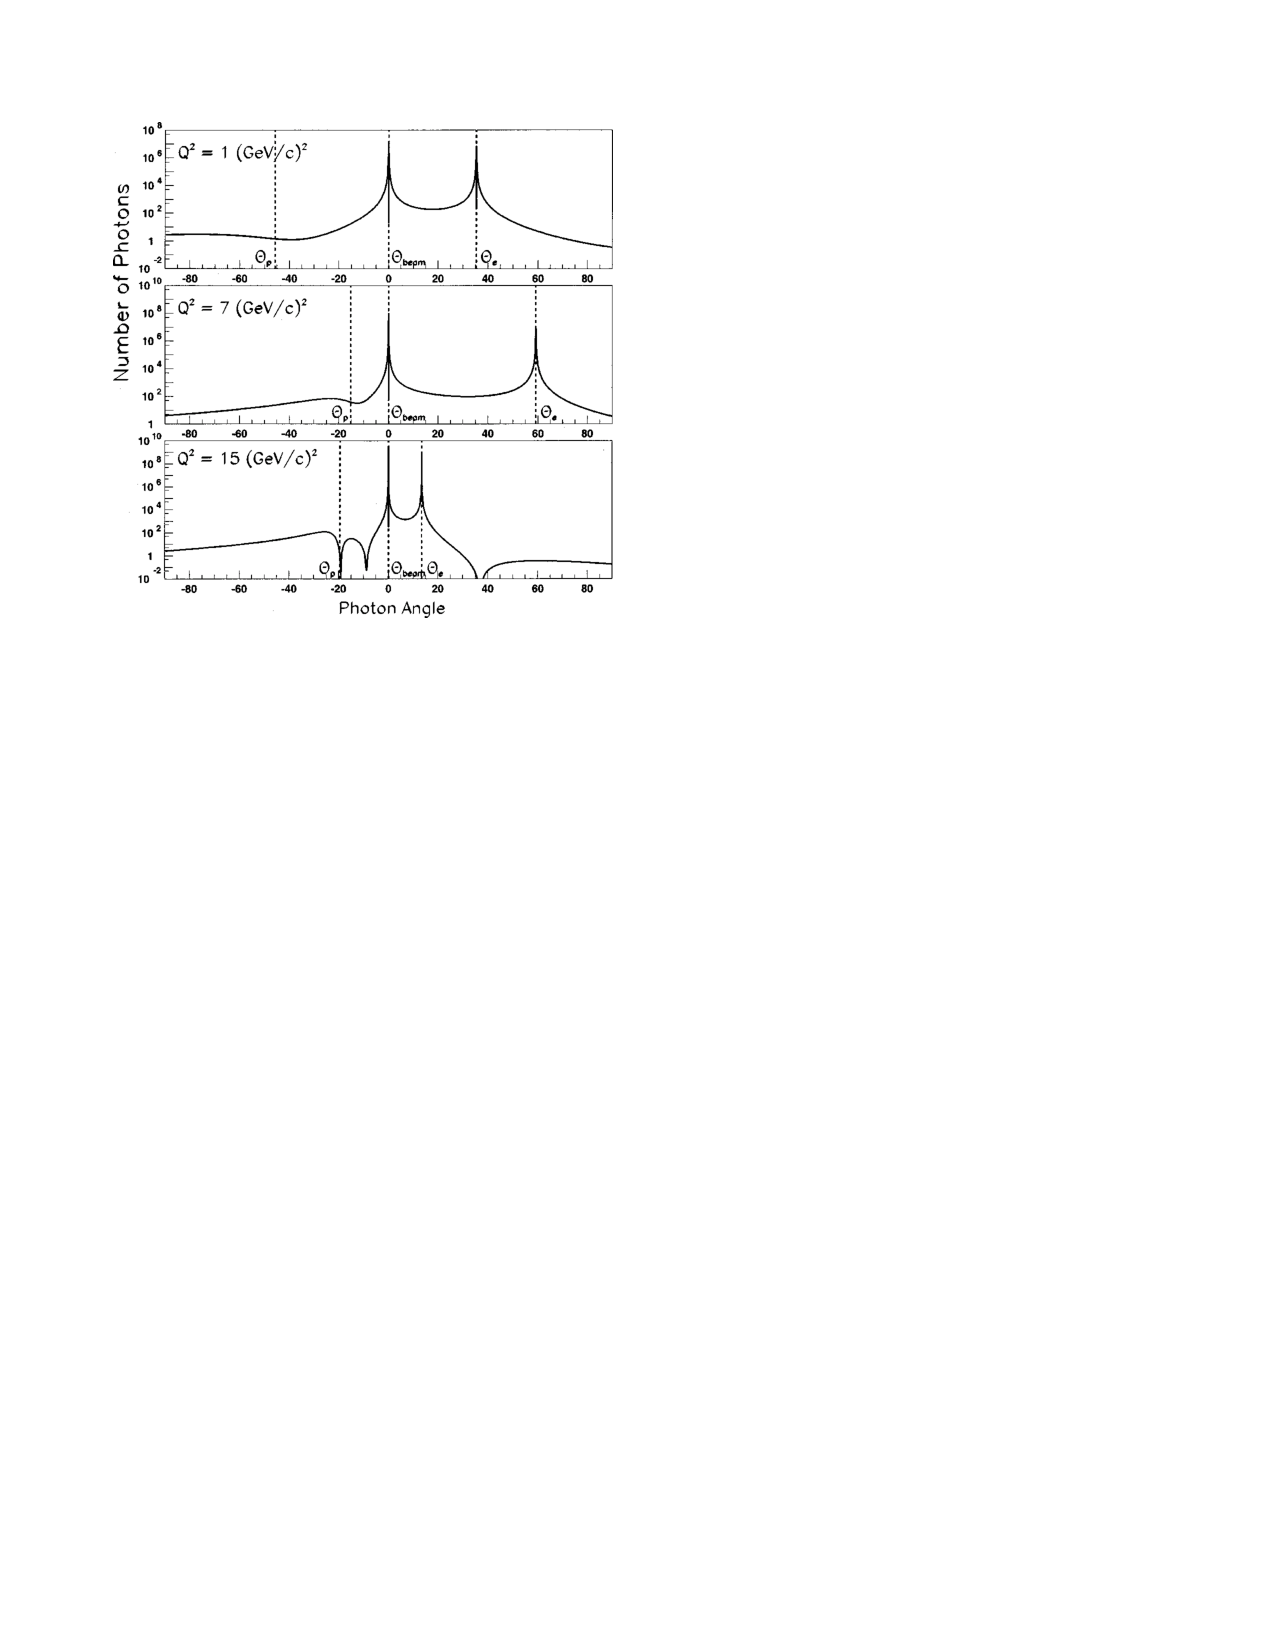
\includegraphics[width=0.7\textwidth]{chap1/single_photon_angular_distribution.pdf}
    \caption{The angular distribution of first order single photon
             Bremmstrahlung for three values of momentum transfer $Q^2$.
             The photon angle, given in degrees, is measured with respect to
             the direction of the incoming beam electron.
             The directions $\theta_e$ and $theta_p$ of the scattered electron
             and proton are indicated by dotted lines.
             Figure reproduced from Ref~\cite{Ent_2001}.
             }
    \label{fig:single_photon_angular_distribution}
\end{figure}

As shown in Fig~\ref{fig:single_photon_angular_distribution}, the single
photon angular distribution is peaked around the directions of the incoming and
outgoing electron, and this focus increases with momentum transfer $Q^2$.
A broad peak in the direction of the scattered proton also becomes more defined
with increasing $Q^2$.
The \textit{peaking approximation} consists of dividing the total energy
radiated in Bremmstrahlung into three photons of energy $E_e$, $E_{e'}$, and
$E_{p'}$ that travel in the directions
$\hat{k}$ of the incoming electron,
$\hat{k}'$ of the outgoing electron,
and
$\hat{p}'$ of the outgoing proton.
The angular distribution $A(\hat{\omega})$ then becomes
\begin{equation}
    A_{peaking}(\hat{\omega}) = \lambda_{e}  \delta(\hat{\omega}-\hat{k}) +
                                \lambda_{e'} \delta(\hat{\omega}-\hat{k}') +
                                \lambda_{p'} \delta(\hat{\omega}-\hat{p}')
\end{equation}
The form of these $\lambda_i$ terms can be found by breaking up the angular
distribution $A(\hat{\omega})$ into three terms---one due to electron, one
due to the proton, and one with the cross terms

\begin{align}
    A(\hat{\omega}) = -\frac{\alpha(\omega^0)^2}{4\pi^{2}}
                        &\left[\left(\frac{k^{\prime}}{\omega \cdot k^{\prime}}-\frac{k}{\omega \cdot k}\right)^{2}
                        + \left(\frac{p^{\prime}}{\omega \cdot p^{\prime}}-\frac{p}{\omega \cdot p}\right)^{2}\right.\nonumber\\
                        &\left.-2\left(\frac{k^{\prime}}{\omega \cdot k^{\prime}}-\frac{k}{\omega \cdot k}\right)
                        \left(\frac{p^{\prime}}{\omega \cdot p^{\prime}}-\frac{p}{\omega \cdot p}\right) \right]
\end{align}

By expanding each of these terms in the polar coordinate $\theta$,
making approximations about their asymptotic behavior near and away from the peaks,
and finally integrating them, one can distribute their contents among the three
directions
\begin{align}
    \lambda_e    &= \frac{\alpha}{\pi}\left[\log\left(\frac{4k^2}{m_e^2}\right) +
                                        2\log\left(\frac{k}{k'}\right) +
                                        \log\left(\frac{1-cos\theta_e}{2}\right)
                                        -1\right] \\
    \lambda_{e'} &= \frac{\alpha}{\pi}\left[\log\left(\frac{4k'^2}{m_e^2}\right) +
                                        2\log\left(\frac{k}{k'}\right) +
                                        \log\left(\frac{1-cos\theta_e}{2}\right)
                                        -1\right] \\
    \lambda_{p'} &= \frac{\alpha}{\pi}
                  \left[
                      \frac{p'^0}{|\vec{p}|}
                      \log\left(\frac{p'^0+|\vec{p}|}
                                     {p'^0-|\vec{p}|}\right)
                      - 2
                  \right]
\end{align}

Generalizing to multiphoton Bremsstrahlung,
\begin{align}
    \frac{d\sigma}{d\Omega_e dE_e dE_{e'} dE_{p'}} &= \left. \frac{d\sigma^{(1)}}{d\Omega_e}\right|_{ep} \left(1-\delta_{hard}\right) \\
    &\times\frac{\lambda_e \lambda_{e'} \lambda_{p'}} {\left(kk'\right)^{\lambda_e/2} \left(kk'\right)^{\lambda_{e'}/2} \left(m_p p'^0\right)^{\lambda_{p'}/2}} \\
    &\times\frac{1}{E_{e}^{1-\lambda_{e}} E_{e'}^{1-\lambda_{e'}} E_{p'}^{1-\lambda_{p'}}}
\end{align}

\subsection{External Bremsstrahlung}
% our flags:
% rad_flag = 0; "use best available formulas, generate in (ntail,Egamma) basis"
% extrad_flag = 2; "use BASIC ext rad formulas x phi"
External Bremsstrahlung refers to the emission of photons in the fields of
nuclei other than the nucleus participating in the primary scattering.
The proton emits a negligible amount of such radiation, but the electron will
experience these losses as it travels through various materials\footnote{
SIMC calculates external Bremsstrahlung for the region between the target
chamber entrance window and the spectrometer entrance windows.
Energy loss and multiple scattering are the dominant corrections in the magnets
and detectors.}

Early~\cite{Early_1973} provides a numerical solution for the probability that
an electron with momentum $k$ radiates a total energy $E^{ext}$ while traveling
through $t$ radiation lengths of material with atomic number Z,
\begin{equation}
    \frac{1}{\Gamma(1+bt)}
    \frac{bt}{E^{ext}}
    \left(\frac{E^{ext}}{k}\right)^{bt}
    \Phi^{ext}\left(\frac{E^{ext}}{k}\right)
\end{equation}
where $b$ is a parameter expressing the $Z$ dependence,
\begin{equation}
    b = \frac{1}{9}\left(12 + \frac{Z+1}{ZL_1+L_2}\right)
\end{equation}
where
$L_1 = \ln{184.15} - \frac{1}{3} \ln Z$
and
$L_2 = \ln{1194} - \frac{2}{3} \ln Z$.
The function $\Phi^{ext}$ is a correction for large photon energies.
For the incoming electron, \textit{SIMC} uses the approximate form
\begin{equation}
    \Phi^{ext}_e\left(\frac{E_e}{k}\right) = 1 - \frac{bt}{bt-\lambda_e}\frac{E_e}{k}
\end{equation}


\textit{SIMC} combines the internal and external Bremsstrahlung into three
photon energies $E_e$, $E_{e'}$, and $E_{p'}$
\begin{align}
\frac{d\sigma}{d\Omega_{e} dE_{e} dE_{e'} dE_{p'}} =&\left.\frac{d\sigma}{d\Omega_{e}}\right|_{ep} \left(1-\delta_{hard}\right) \\
    &\times \frac{1}{\Gamma\left(1+b t_{e}\right)}  \frac{bt_{e}  + \lambda_{e}} {k^{bt_{e}} (kk')^{\lambda_{e}/2}}  \frac{1}{E_{e}^{1 -\lambda_{e} -bt_{e}}} \\
    &\times \frac{1}{\Gamma\left(1+b t_{e'}\right)} \frac{bt_{e'} + \lambda_{e'}}{k^{bt_{e'}}(kk')^{\lambda_{e'}/2}} \frac{1}{E_{e'}^{1-\lambda_{e'}-bt_{e'}}} \\
    &\times \frac{\lambda_{p'}}{(m_p p')^{\lambda_{p'}/2}} \frac{1}{E_{p'}^{1-\lambda_{p'}}}
\end{align}

Using the energy distributions contained in this expression,
\textit{SIMC} generates the radiated energy based on the limits
$E_{min}$ and $E_{max}$
imposed by
the model spectral functions,
spectrometer acceptances,
and randomly generated initial and final 4-momenta of particles participating
in scattering.
These energies are then subtracted from the particles' vertex energies.


Then, \textit{SIMC} generates a weight $W^{event}_{rad}$ for the event based on the
probabilities of emitting energies $E_i$, where $i$ is one of $e$, $e'$, and
$p'$.
The first contribution to this weight,
$W^{soft}_{rad}=W^{e}_{rad}W^{e'}_{rad}W^{p'}_{rad}$, is due to Bremsstrahlung,
where
\begin{equation}
    W^{e}_{rad} = \frac{1}{\Gamma(1+bt_{e})} \frac{1}{k^{bt_{e}}(kk')^{\lambda_{e}/2}}
                \left((E^{e}_{max})^{bt+\lambda_{e}}-(E^{e}_{max})^{bt+\lambda_{e}}\right)
\end{equation}
\begin{equation}
    W^{e'}_{rad} = \frac{1}{\Gamma(1+bt_{e'})} \frac{1}{k^{bt_{e'}}(kk')^{\lambda_{e'}/2}}
                \left((E^{e'}_{max})^{bt+\lambda_{e'}}-(E^{e'}_{max})^{bt+\lambda_{e'}}\right)
\end{equation}
\begin{equation}
    W^{p'}_{rad} =  \frac{1}{(m_p p')^{\lambda_{p'}/2}}
                \left((E^{p'}_{max})^{\lambda_{p'}}-(E^{p'}_{max})^{\lambda_{p'}}\right)
\end{equation}

The second contribution $\Phi^{ext}=\Phi^{ext}_{e}\Phi^{ext}_{e'}$
is due to external radiation.
The final contribution $(1-\delta_{hard})$ is due to vertex corrections.
Altogether, the weight from radiative corrections is
\begin{equation}
    W_{rad} = W^{soft}_{rad} \Phi^{ext} (1-\delta_{hard})
\end{equation}


\section{Multiple Scattering}

\textit{SIMC} includes a list of the effective thickness in radiation lengths
$t_{eff}$ of every material a particle passes through.
As the simulated particle with momentum $p$ passes through each material, a
rescattering angle $\theta$ is calculated using the approximation of
Moli\`{e}re's multiple scattering theory given in Equation (6) of
Ref~\cite{Lynch_1991},
\begin{equation}
    \theta = \frac{E_s}{p \beta}
             \sqrt{t_{eff}}
             \left[1 + \epsilon \log_{10}{\left( \frac{t_{eff}}{\beta^2} \right)}\right]
\end{equation}
where $E_s=\SI{13.6}{\mega\electronvolt}$ and $\epsilon=0.088$ are parameters
taken from fits to multiple scattering measurements taken at
Fermilab~\cite{Shen_1979}.
These measurements were taken with incident pions, kaons, and protons at
momenta between 50 and \SI{200}{\giga\electronvolt} on hydrogen, beryllium,
carbon, aluminum, copper, tin, and lead targets.

\section{Energy Loss}
Energy loss in \si{\mega\electronvolt} is determined by the Bethe-Bloch formula,
the implementation of which can currently be found in \texttt{enerloss\_new.f}.
\begin{equation}
 E_{loss} =  K \frac{Z}{A} \frac{t}{\beta^2}
             \left[
                1.063
                + \log\left(\frac{m_e}{I^2}\right)
                + 2 \log(\gamma\beta)
                - \beta^2
                + \log\left(K\frac{Z}{A}\frac{t}{\beta^2}\right)
                - \delta
             \right]
\end{equation}
where
$K=\SI{0.1536e-03}{\centi\meter\squared\per\gram}$,
$t$ is the thickness of the material in \si{\gram\per\centi\meter\squared},
$Z$ and $A$ are the effective atomic number and weight of the material,
$I=16 Z^{0.9}) \si{\electronvolt}$ is the estimated ionization energy of the material,
and $\delta$ is a momentum-dependent density effect correction.
% Why 1.063? Trying to make sense of this and Leo secton 2.2.2

The density effect arises from the fact that a charged particle will polarize
the atoms in the material along its path.
Electrons in atoms far from this path will be shielded and contribute less to
the total energy loss.
The magnitude of this effect is greater at larger momenta.

% \section{Weighting and Normalization}
% \begin{equation}
%     \text{normfac} = \frac{\mathcal{L} \Delta E_p \Delta \Omega_p \Delta E_e \Delta \Omega_e}
%                           {N_{gen}}
% \end{equation}

\chapter{Comparison of Experimental and Monte Carlo Distributions} \label{app:distributions}
This appendix compares the distributions of reconstructued quantities measured in experiment
to those generated by \textit{SIMC}.
Error bars are statistical only and the distributions are normalized to each other.
\begin{figure}[!h]
    \centering
    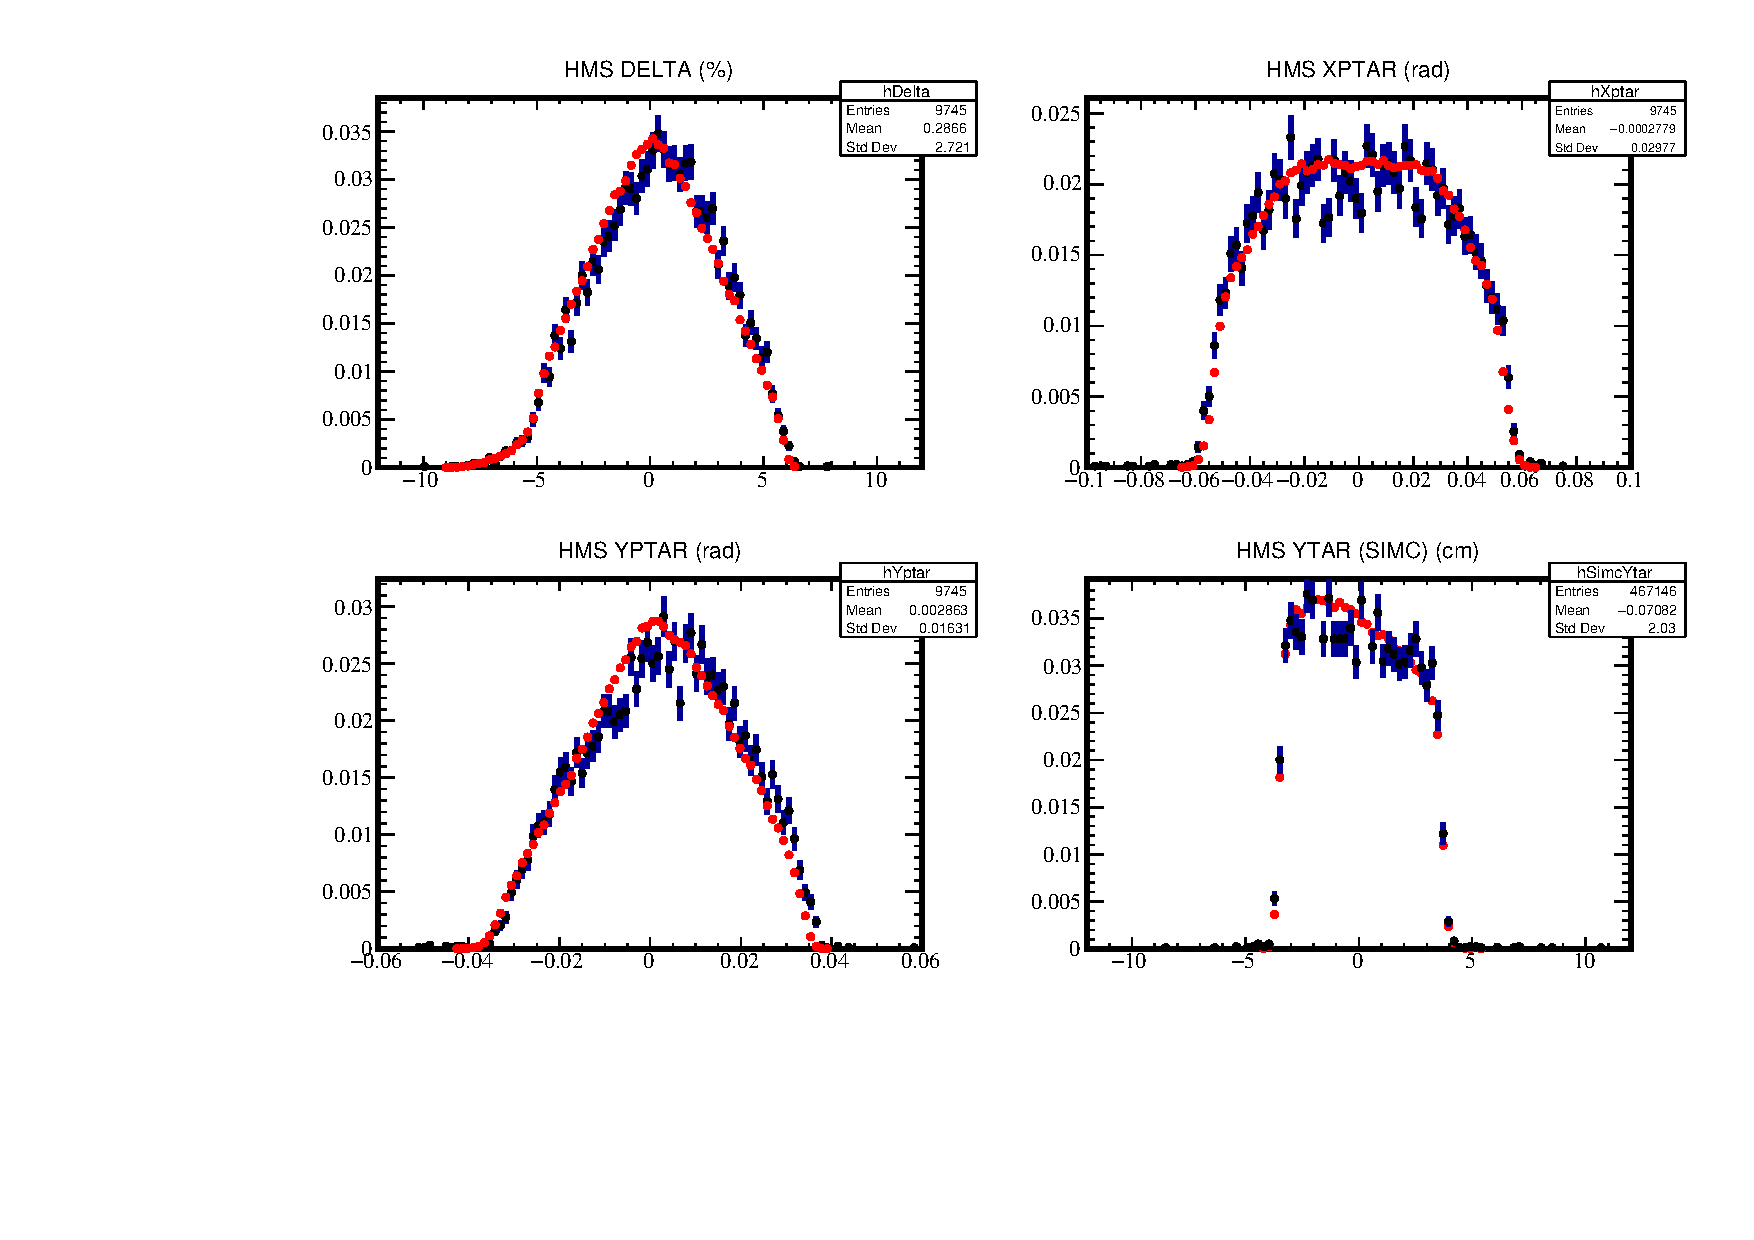
\includegraphics[page=1,width=1.0\textwidth]{pass5_report/Report_h8.pdf}
    \caption{
            Experimental (in blue) and Monte Carlo (in red) distributions of
            target quantities reconstructed from the HMS for
            the $LH_2$ target at $Q^2=\SI{8.0}{\giga\electronvolt\squared}$.
            }
    \label{fig:Report_h8.pdf}
\end{figure}


\begin{figure}[!h]
    \centering
    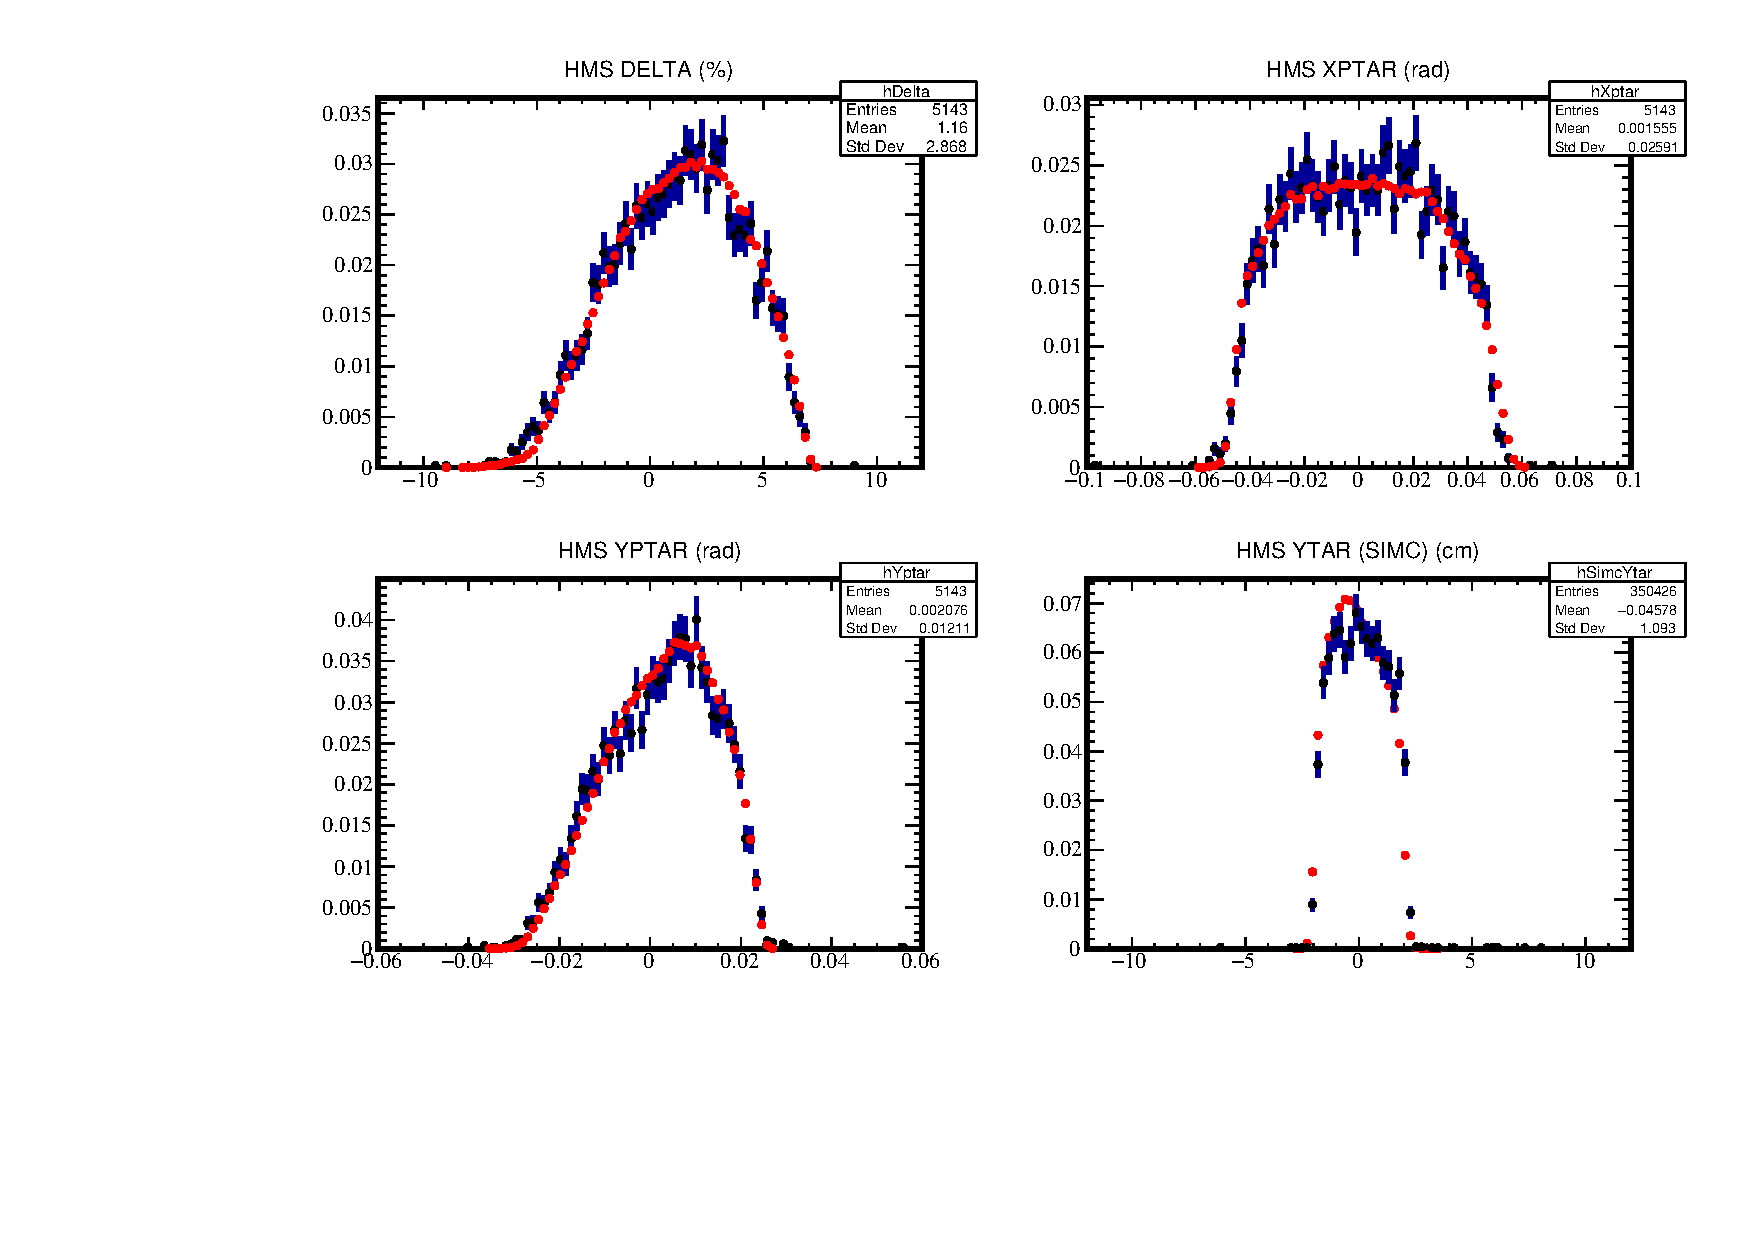
\includegraphics[page=1,width=1.0\textwidth]{pass5_report/Report_h95sm.pdf}
    \caption{
            Experimental (in blue) and Monte Carlo (in red) distributions of
            target quantities reconstructed from the HMS for
            the $LH_2$ target at $Q^2=\SI{9.5}{\giga\electronvolt\squared}$.
            }
    \label{fig:Report_h95sm.pdf}
\end{figure}


\begin{figure}[!h]
    \centering
    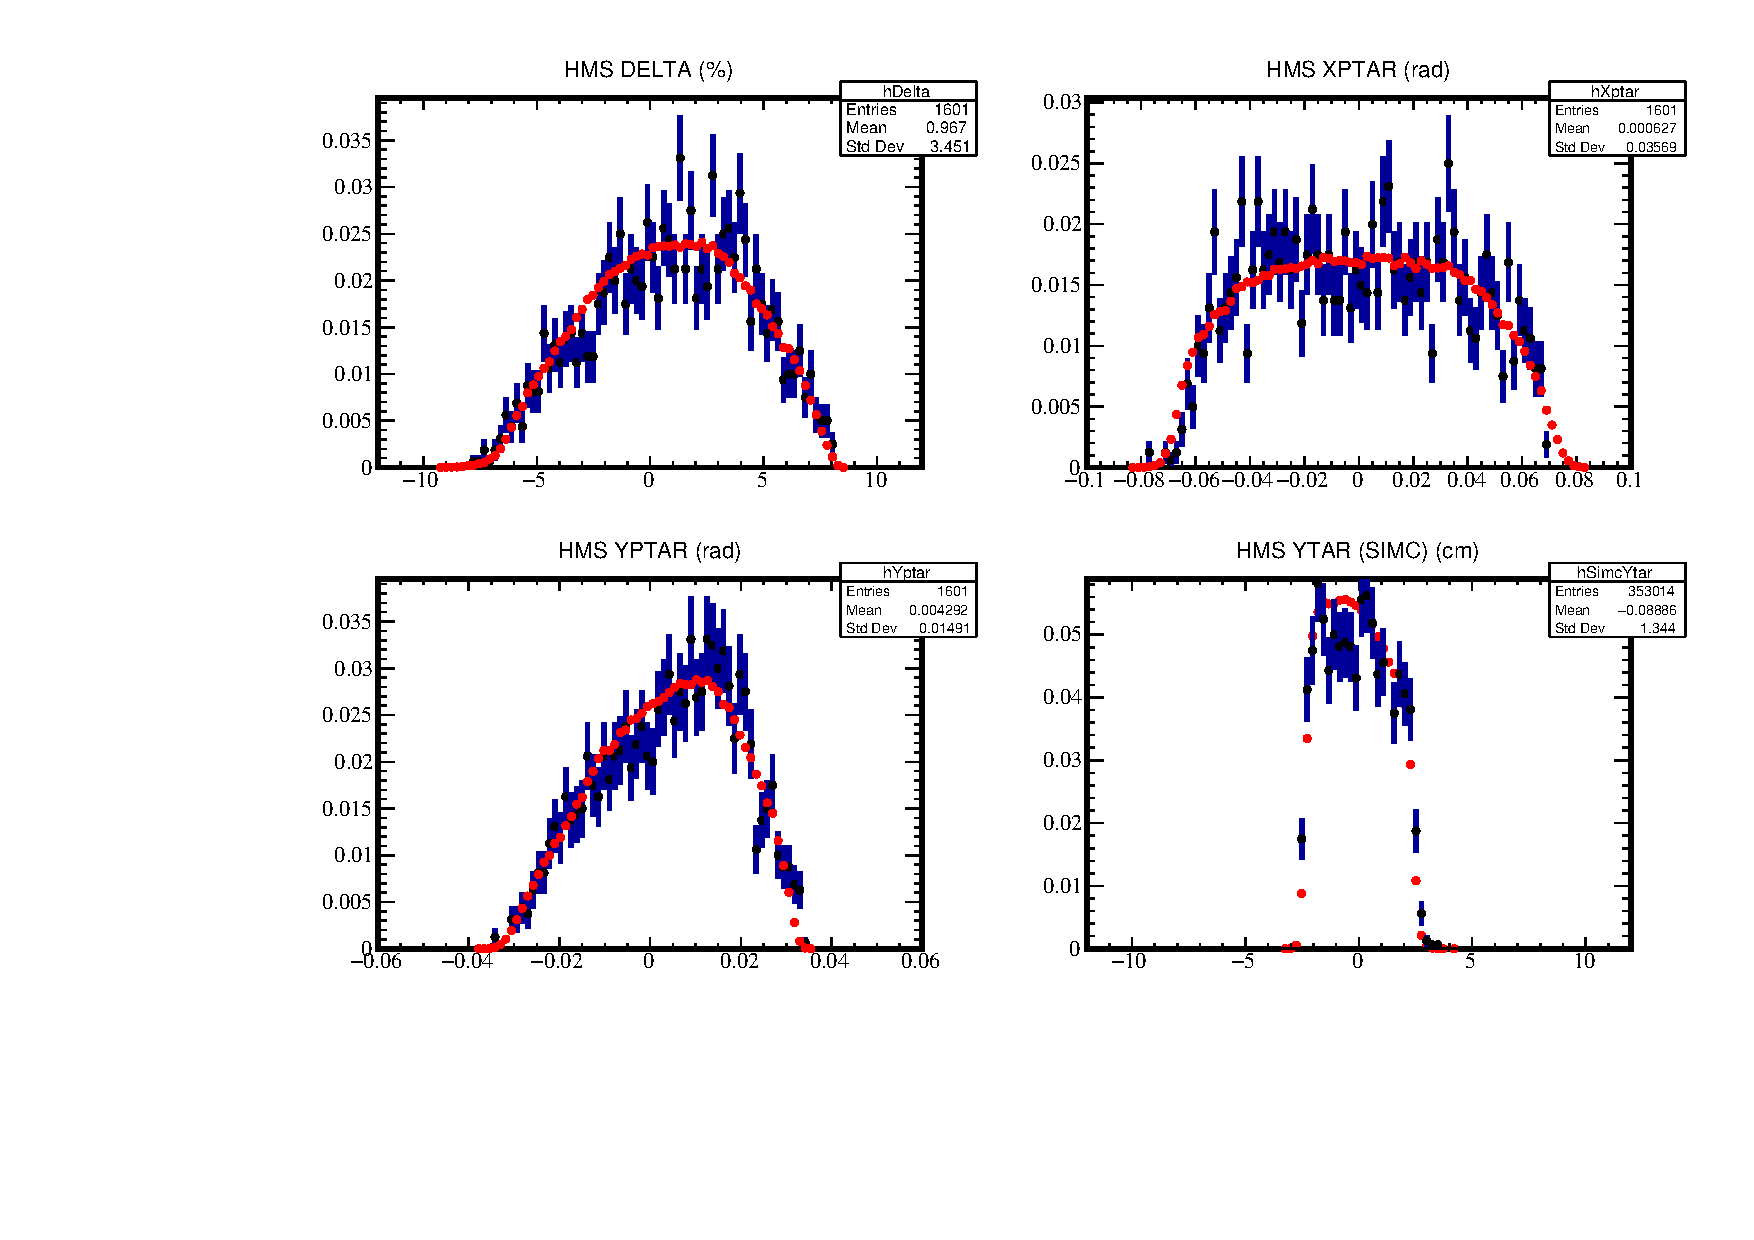
\includegraphics[page=1,width=1.0\textwidth]{pass5_report/Report_h115.pdf}
    \caption{
            Experimental (in blue) and Monte Carlo (in red) distributions of
            target quantities reconstructed from the HMS for
            the $LH_2$ target at $Q^2=\SI{11.5}{\giga\electronvolt\squared}$.
            }
    \label{fig:Report_h115.pdf}
\end{figure}


\begin{figure}[!h]
    \centering
    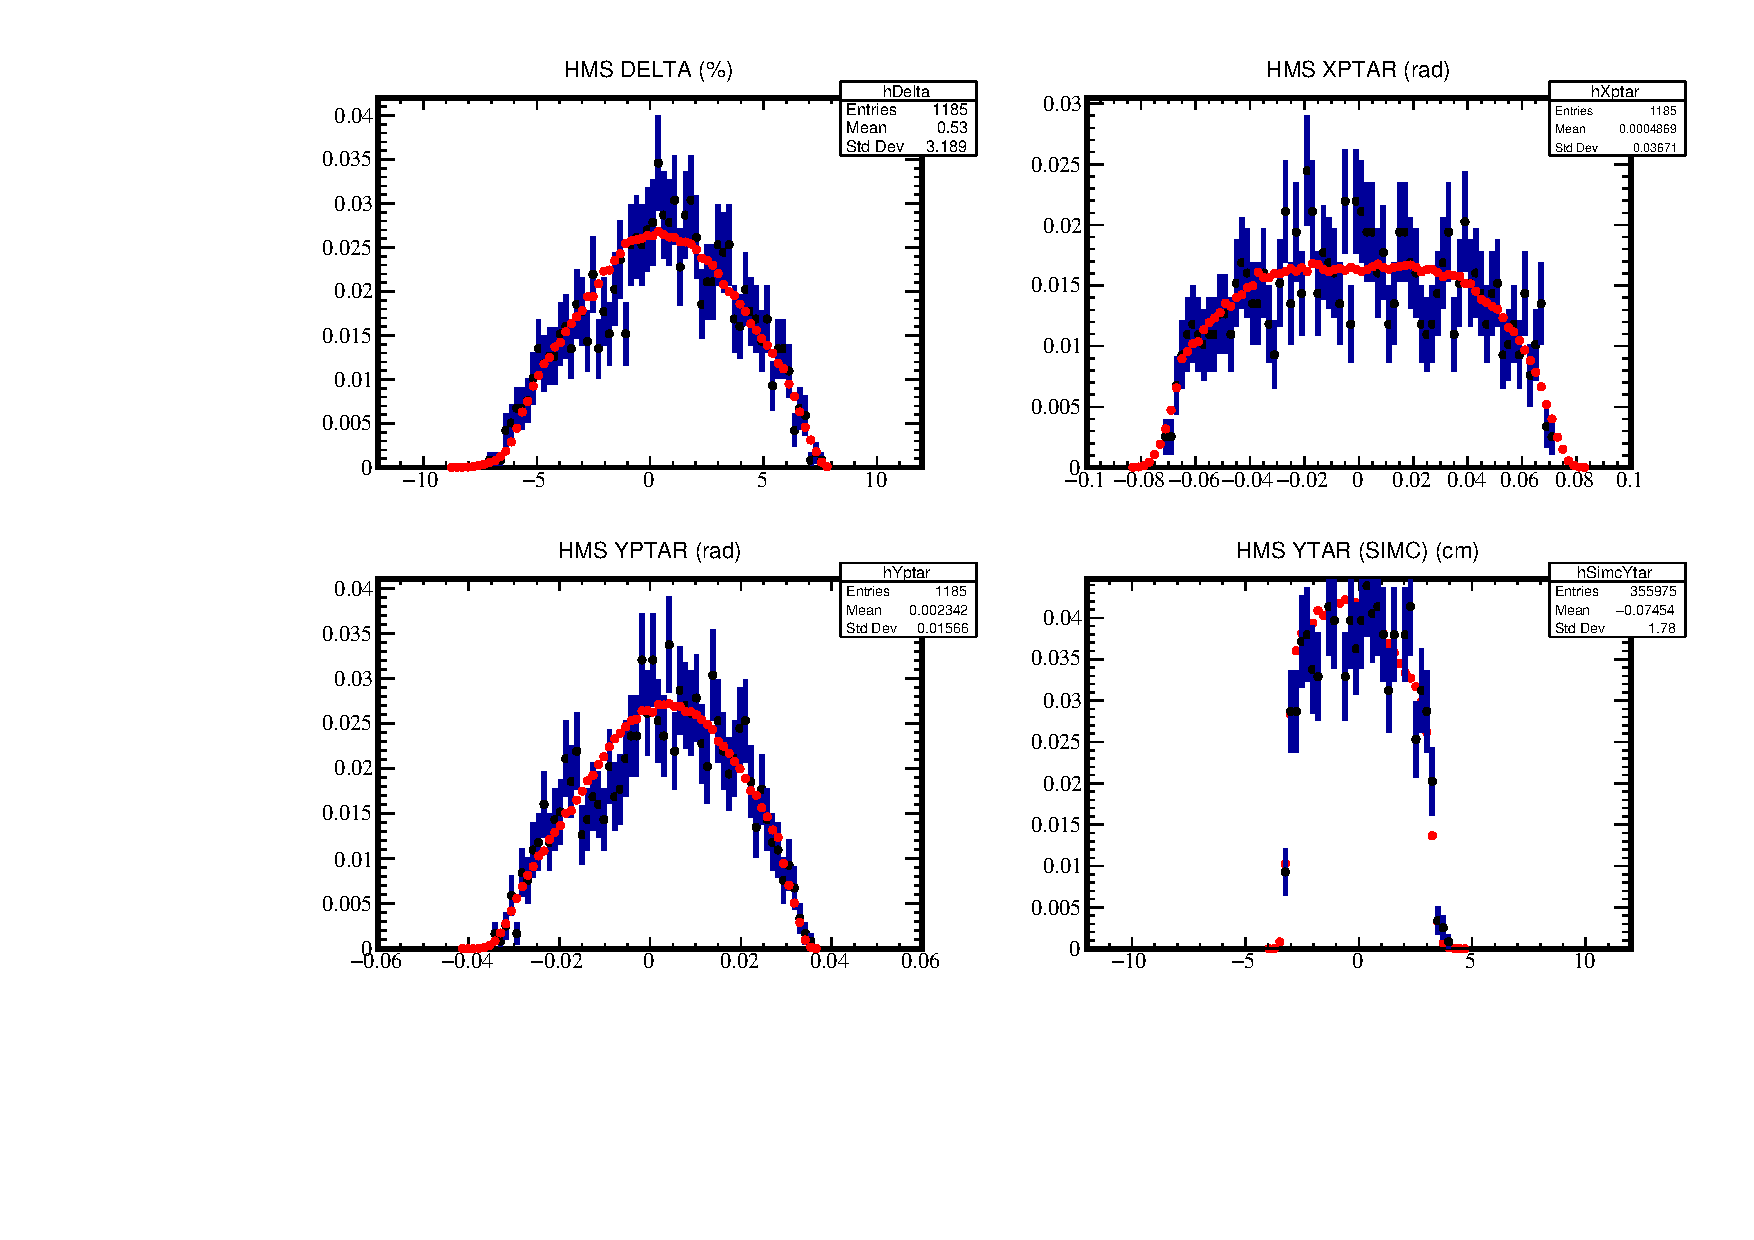
\includegraphics[page=1,width=1.0\textwidth]{pass5_report/Report_h143.pdf}
    \caption{
            Experimental (in blue) and Monte Carlo (in red) distributions of
            target quantities reconstructed from the HMS for
            the $LH_2$ target at $Q^2=\SI{14.2}{\giga\electronvolt\squared}$.
            }
    \label{fig:Report_h143.pdf}
\end{figure}


\begin{figure}[!h]
    \centering
    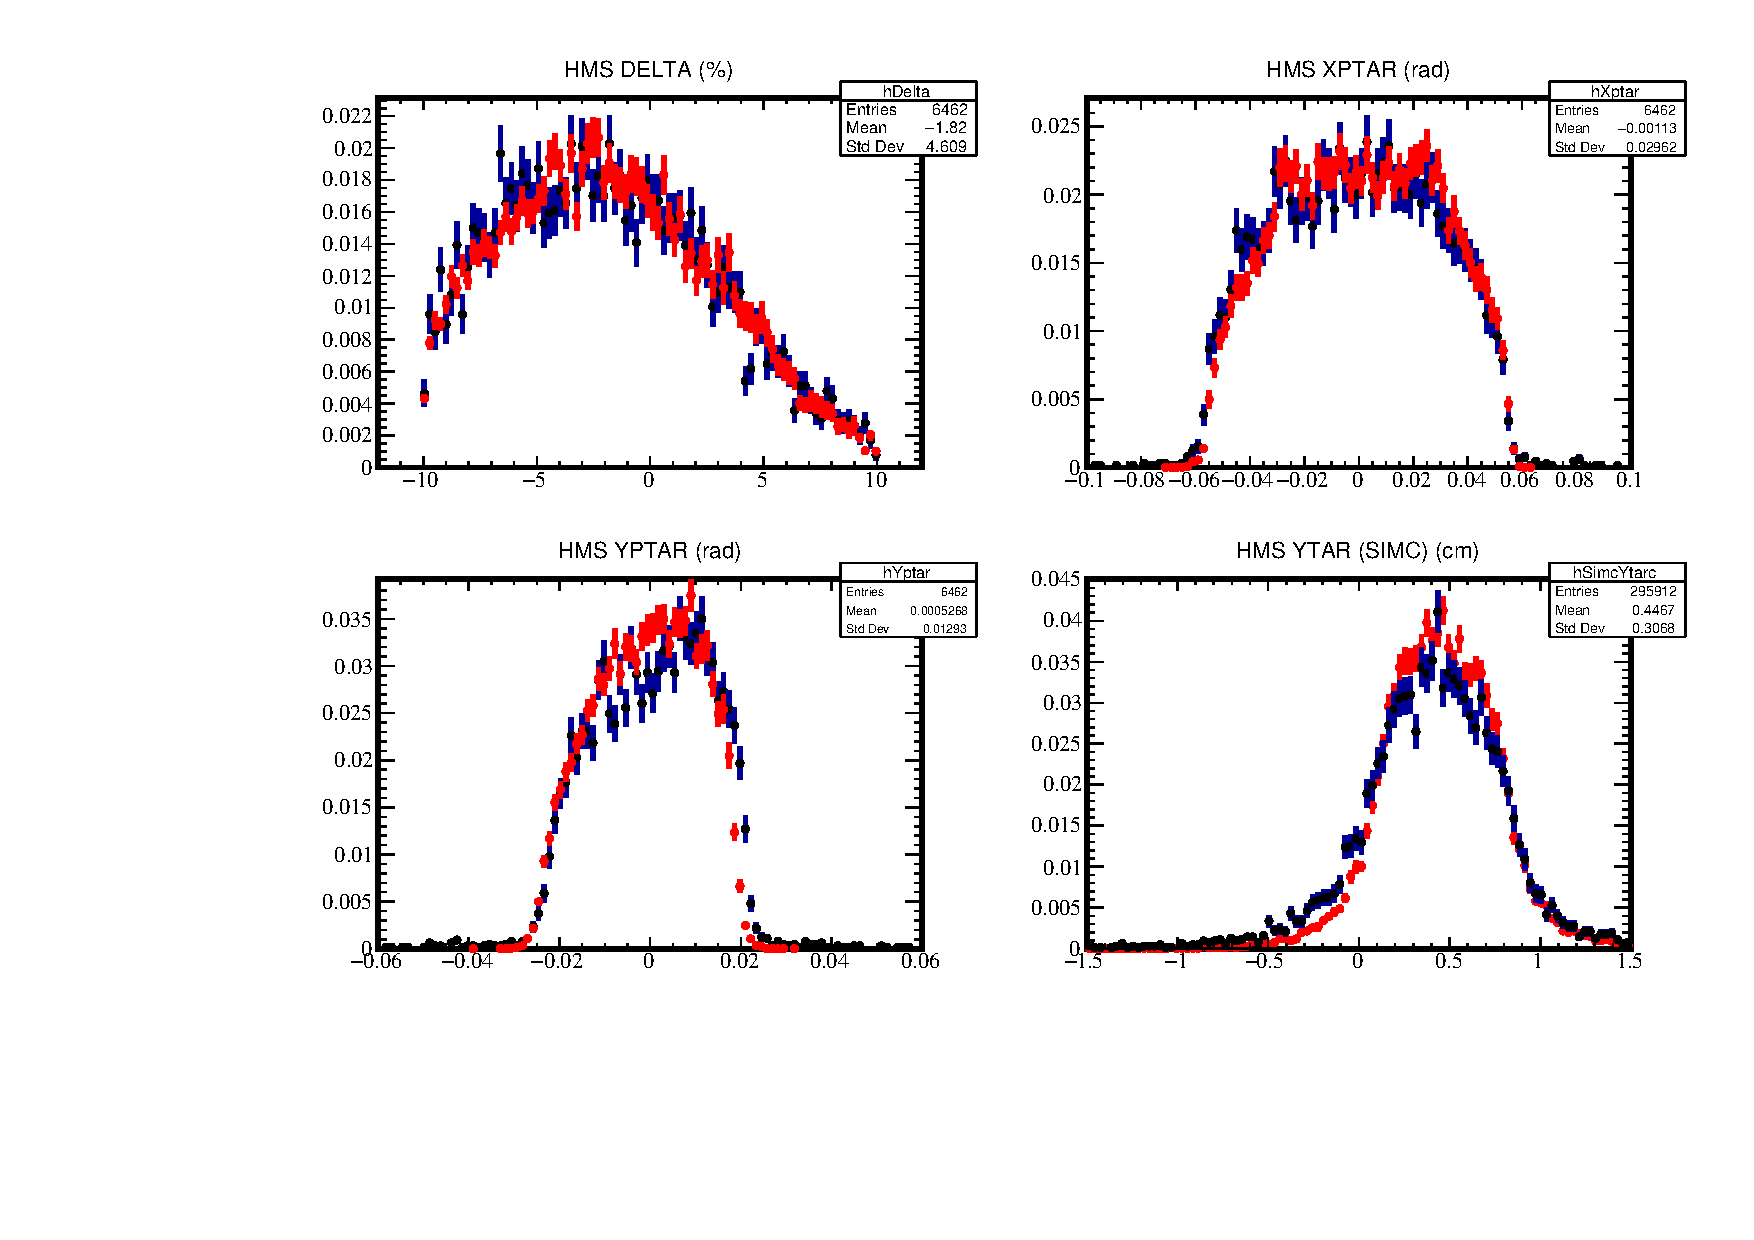
\includegraphics[page=1,width=1.0\textwidth]{pass5_report/Report_c12_8.pdf}
    \caption{
            Experimental (in blue) and Monte Carlo (in red) distributions of
            target quantities reconstructed from the HMS for
            the ${}^{12}C$ target at $Q^2=\SI{8.0}{\giga\electronvolt\squared}$.
            }
    \label{fig:Report_c12_8.pdf}
\end{figure}


\begin{figure}[!h]
    \centering
    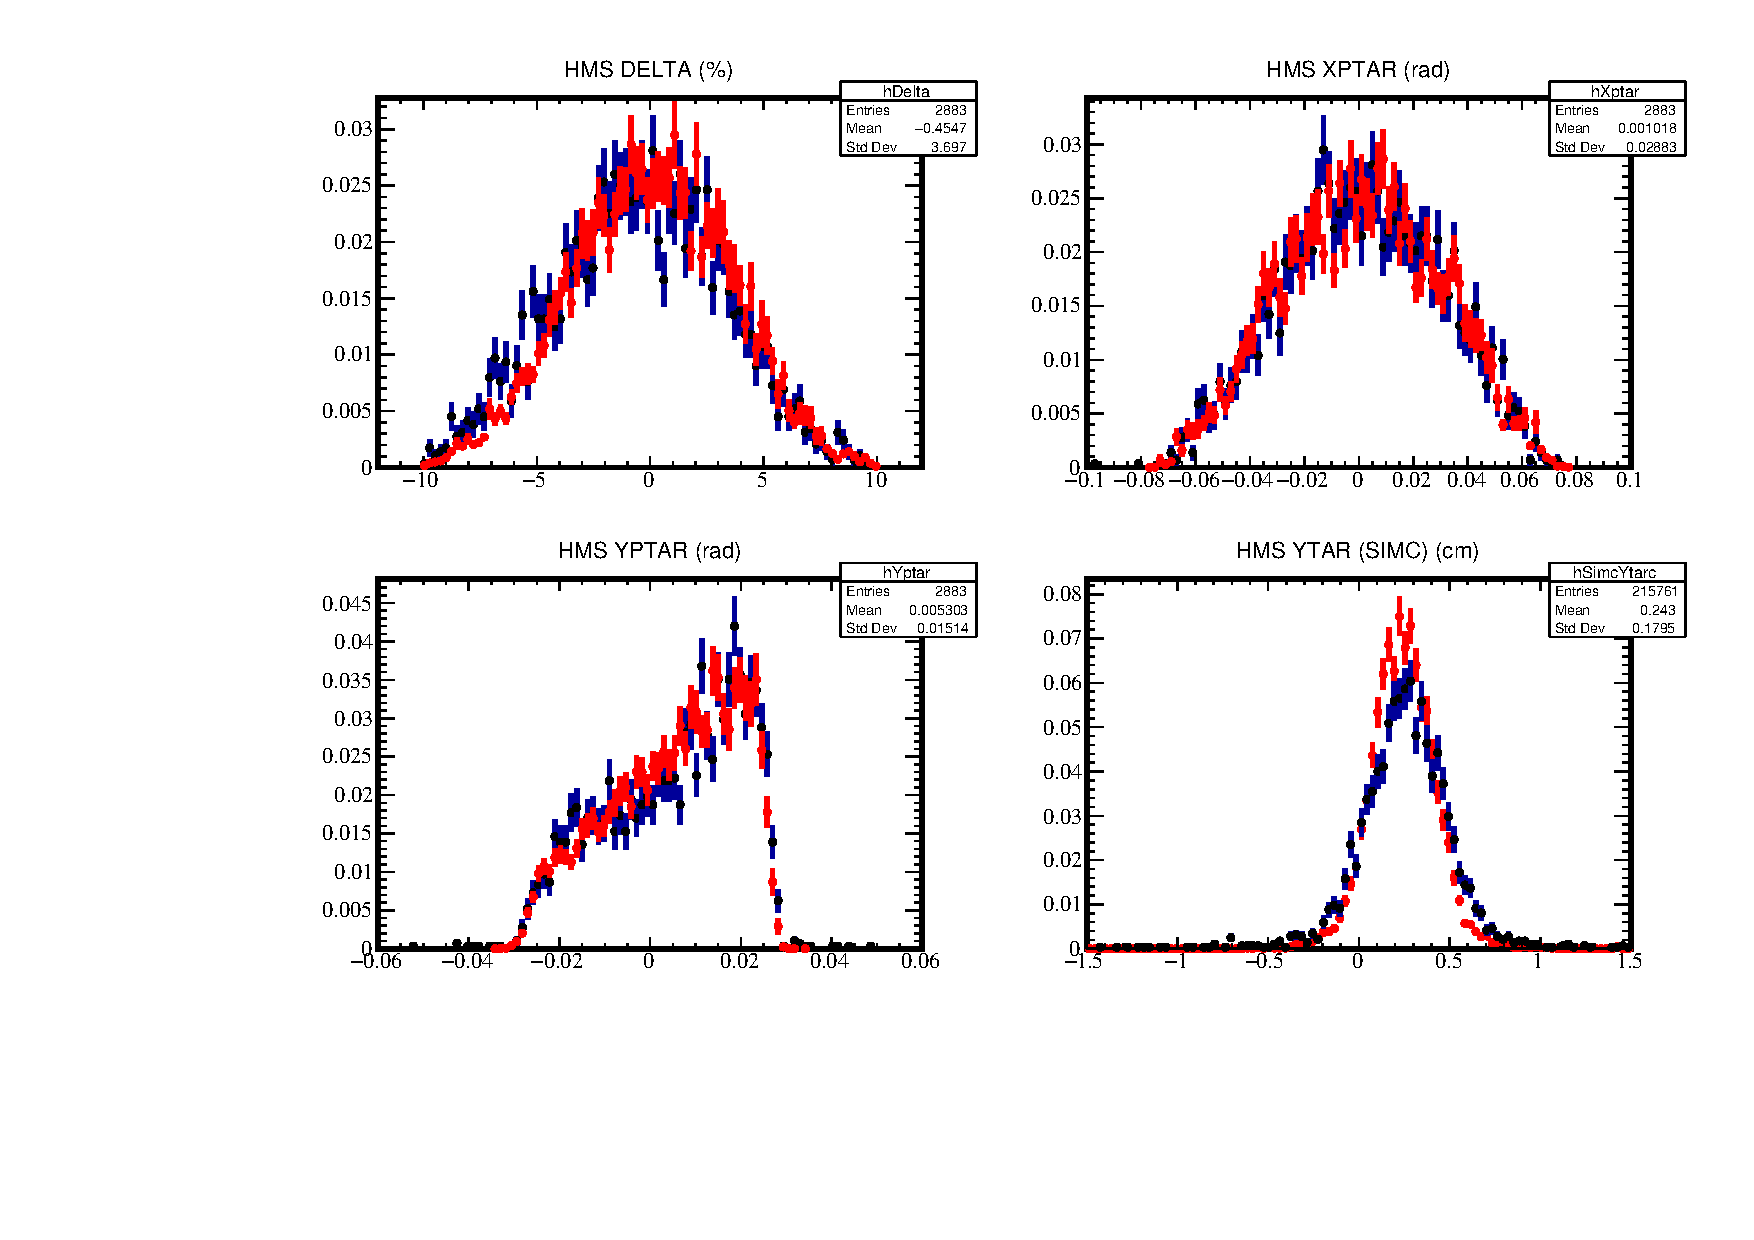
\includegraphics[page=1,width=1.0\textwidth]{pass5_report/Report_c95.pdf}
    \caption{
            Experimental (in blue) and Monte Carlo (in red) distributions of
            target quantities reconstructed from the HMS for
            the ${}^{12}C$ target at $Q^2=\SI{9.5}{\giga\electronvolt\squared}$.
            }
    \label{fig:Report_c95.pdf}
\end{figure}


\begin{figure}[!h]
    \centering
    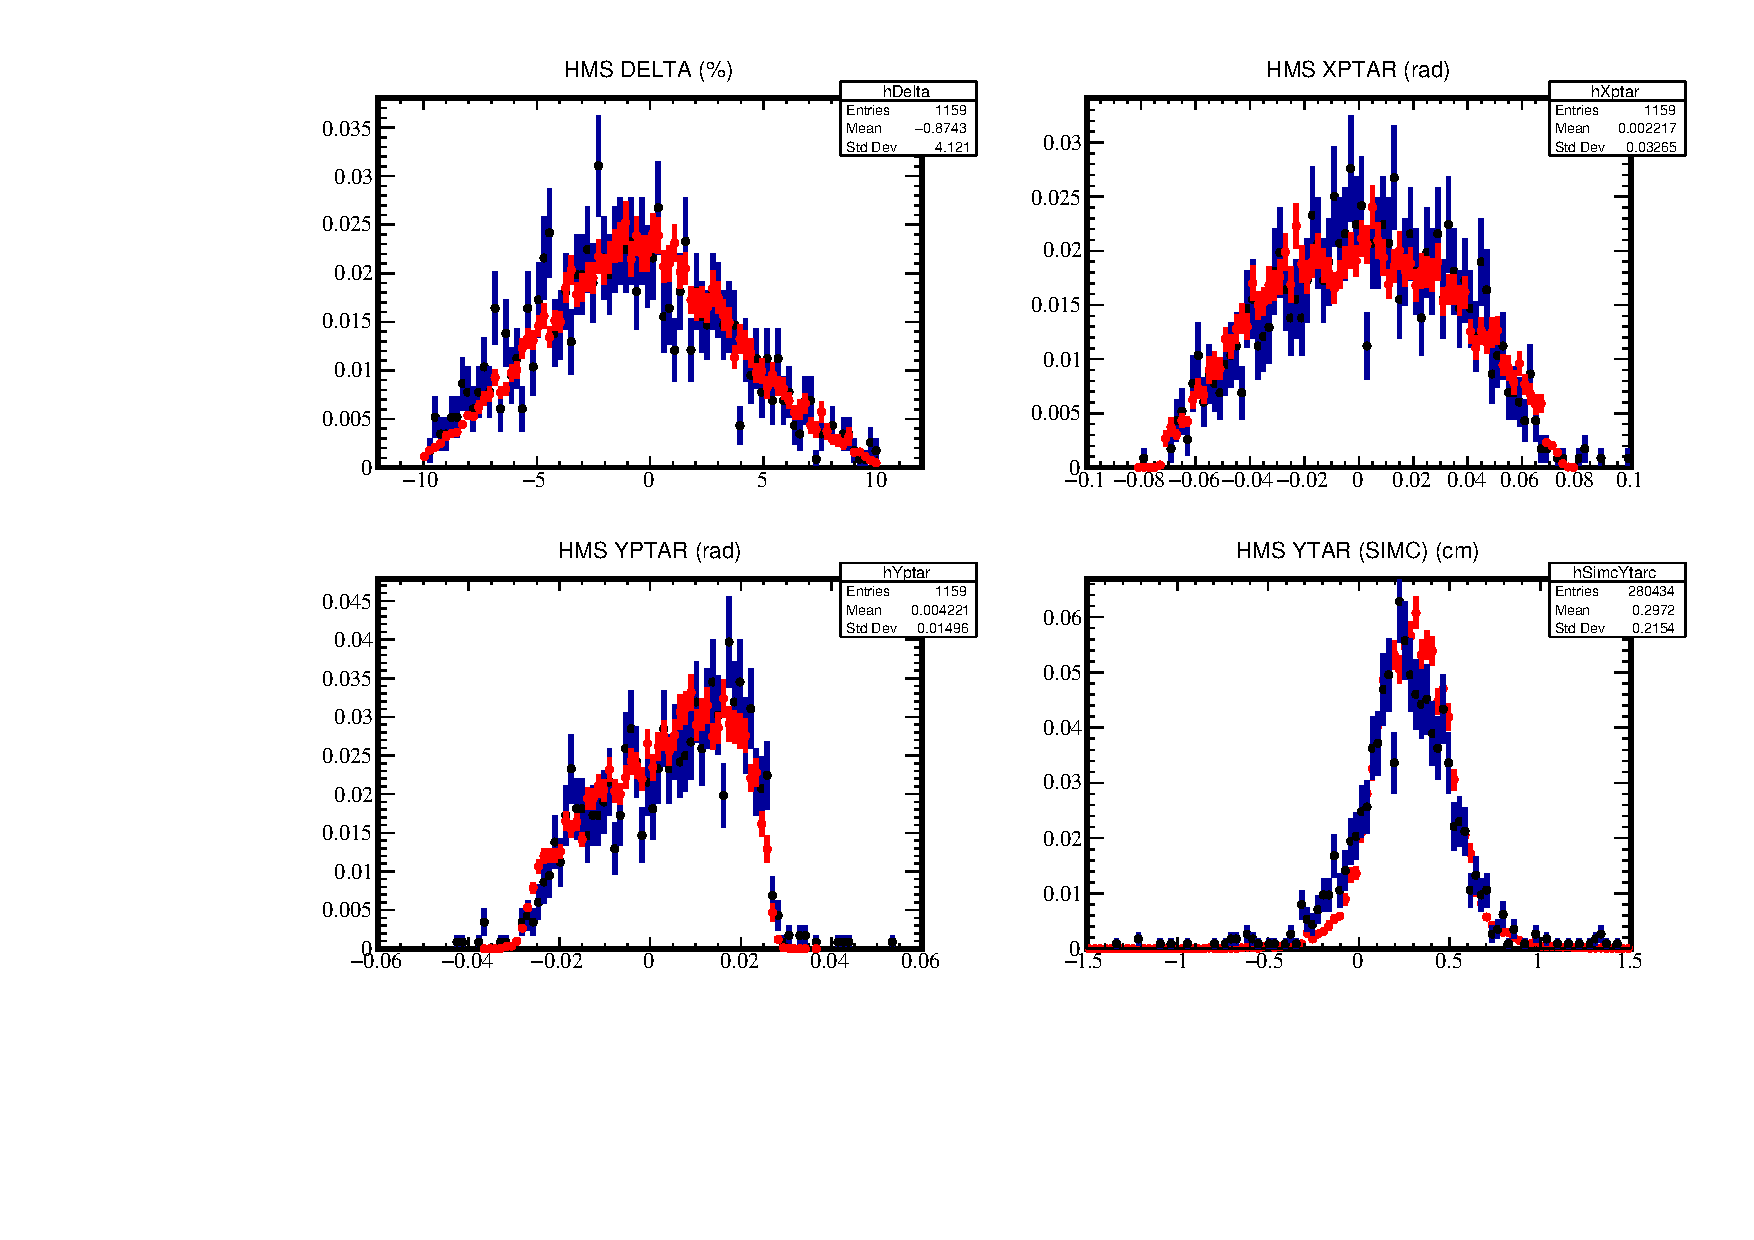
\includegraphics[page=1,width=1.0\textwidth]{pass5_report/Report_c115.pdf}
    \caption{
            Experimental (in blue) and Monte Carlo (in red) distributions of
            target quantities reconstructed from the HMS for
            the ${}^{12}C$ target at $Q^2=\SI{11.5}{\giga\electronvolt\squared}$.
            }
    \label{fig:Report_c115.pdf}
\end{figure}


\begin{figure}[!h]
    \centering
    \includegraphics[page=1,width=1.0\textwidth]{pass5_report/Report_c143_sm.pdf}
    \caption{
            Experimental (in blue) and Monte Carlo (in red) distributions of
            target quantities reconstructed from the HMS for
            the ${}^{12}C$ target at $Q^2=\SI{14.2}{\giga\electronvolt\squared}$.
            }
    \label{fig:Report_c143_sm.pdf}
\end{figure}


\begin{figure}[!h]
    \centering
    \includegraphics[page=2,width=1.0\textwidth]{pass5_report/Report_h8.pdf}
    \caption{
            Experimental (in blue) and Monte Carlo (in red) distributions of
            target quantities reconstructed from the SHMS for
            the $LH_2$ target at $Q^2=\SI{8.0}{\giga\electronvolt\squared}$.
            }
    \label{fig:Report_h8.pdf}
\end{figure}


\begin{figure}[!h]
    \centering
    \includegraphics[page=2,width=1.0\textwidth]{pass5_report/Report_h95sm.pdf}
    \caption{
            Experimental (in blue) and Monte Carlo (in red) distributions of
            target quantities reconstructed from the SHMS for
            the $LH_2$ target at $Q^2=\SI{9.5}{\giga\electronvolt\squared}$.
            }
    \label{fig:Report_h95sm.pdf}
\end{figure}


\begin{figure}[!h]
    \centering
    \includegraphics[page=2,width=1.0\textwidth]{pass5_report/Report_h115.pdf}
    \caption{
            Experimental (in blue) and Monte Carlo (in red) distributions of
            target quantities reconstructed from the SHMS for
            the $LH_2$ target at $Q^2=\SI{11.5}{\giga\electronvolt\squared}$.
            }
    \label{fig:Report_h115.pdf}
\end{figure}


\begin{figure}[!h]
    \centering
    \includegraphics[page=2,width=1.0\textwidth]{pass5_report/Report_h143.pdf}
    \caption{
            Experimental (in blue) and Monte Carlo (in red) distributions of
            target quantities reconstructed from the SHMS for
            the $LH_2$ target at $Q^2=\SI{14.2}{\giga\electronvolt\squared}$.
            }
    \label{fig:Report_h143.pdf}
\end{figure}


\begin{figure}[!h]
    \centering
    \includegraphics[page=2,width=1.0\textwidth]{pass5_report/Report_c12_8.pdf}
    \caption{
            Experimental (in blue) and Monte Carlo (in red) distributions of
            target quantities reconstructed from the SHMS for
            the ${}^{12}C$ target at $Q^2=\SI{8.0}{\giga\electronvolt\squared}$.
            }
    \label{fig:Report_c12_8.pdf}
\end{figure}


\begin{figure}[!h]
    \centering
    \includegraphics[page=2,width=1.0\textwidth]{pass5_report/Report_c95.pdf}
    \caption{
            Experimental (in blue) and Monte Carlo (in red) distributions of
            target quantities reconstructed from the SHMS for
            the ${}^{12}C$ target at $Q^2=\SI{9.5}{\giga\electronvolt\squared}$.
            }
    \label{fig:Report_c95.pdf}
\end{figure}


\begin{figure}[!h]
    \centering
    \includegraphics[page=2,width=1.0\textwidth]{pass5_report/Report_c115.pdf}
    \caption{
            Experimental (in blue) and Monte Carlo (in red) distributions of
            target quantities reconstructed from the SHMS for
            the ${}^{12}C$ target at $Q^2=\SI{11.5}{\giga\electronvolt\squared}$.
            }
    \label{fig:Report_c115.pdf}
\end{figure}


\begin{figure}[!h]
    \centering
    \includegraphics[page=2,width=1.0\textwidth]{pass5_report/Report_c143_sm.pdf}
    \caption{
            Experimental (in blue) and Monte Carlo (in red) distributions of
            target quantities reconstructed from the SHMS for
            the ${}^{12}C$ target at $Q^2=\SI{14.2}{\giga\electronvolt\squared}$.
            }
    \label{fig:Report_c143_sm.pdf}
\end{figure}


\begin{figure}[!h]
    \centering
    \includegraphics[page=3,width=1.0\textwidth]{pass5_report/Report_h8.pdf}
    \caption{
            Experimental (in blue) and Monte Carlo (in red) distributions of
            reconstructed physics quantities for
            the $LH_2$ target at $Q^2=\SI{8.0}{\giga\electronvolt\squared}$.
            }
    \label{fig:Report_h8.pdf}
\end{figure}


\begin{figure}[!h]
    \centering
    \includegraphics[page=3,width=1.0\textwidth]{pass5_report/Report_h95sm.pdf}
    \caption{
            Experimental (in blue) and Monte Carlo (in red) distributions of
            reconstructed physics quantities for
            the $LH_2$ target at $Q^2=\SI{9.5}{\giga\electronvolt\squared}$.
            }
    \label{fig:Report_h95sm.pdf}
\end{figure}


\begin{figure}[!h]
    \centering
    \includegraphics[page=3,width=1.0\textwidth]{pass5_report/Report_h115.pdf}
    \caption{
            Experimental (in blue) and Monte Carlo (in red) distributions of
            reconstructed physics quantities for
            the $LH_2$ target at $Q^2=\SI{11.5}{\giga\electronvolt\squared}$.
            }
    \label{fig:Report_h115.pdf}
\end{figure}


\begin{figure}[!h]
    \centering
    \includegraphics[page=3,width=1.0\textwidth]{pass5_report/Report_h143.pdf}
    \caption{
            Experimental (in blue) and Monte Carlo (in red) distributions of
            reconstructed physics quantities for
            the $LH_2$ target at $Q^2=\SI{14.2}{\giga\electronvolt\squared}$.
            }
    \label{fig:Report_h143.pdf}
\end{figure}


\begin{figure}[!h]
    \centering
    \includegraphics[page=3,width=1.0\textwidth]{pass5_report/Report_c12_8.pdf}
    \caption{
            Experimental (in blue) and Monte Carlo (in red) distributions of
            reconstructed physics quantities for
            the ${}^{12}C$ target at $Q^2=\SI{8.0}{\giga\electronvolt\squared}$.
            }
    \label{fig:Report_c12_8.pdf}
\end{figure}


\begin{figure}[!h]
    \centering
    \includegraphics[page=3,width=1.0\textwidth]{pass5_report/Report_c95.pdf}
    \caption{
            Experimental (in blue) and Monte Carlo (in red) distributions of
            reconstructed physics quantities for
            the ${}^{12}C$ target at $Q^2=\SI{9.5}{\giga\electronvolt\squared}$.
            }
    \label{fig:Report_c95.pdf}
\end{figure}


\begin{figure}[!h]
    \centering
    \includegraphics[page=3,width=1.0\textwidth]{pass5_report/Report_c115.pdf}
    \caption{
            Experimental (in blue) and Monte Carlo (in red) distributions of
            reconstructed physics quantities for
            the ${}^{12}C$ target at $Q^2=\SI{11.5}{\giga\electronvolt\squared}$.
            }
    \label{fig:Report_c115.pdf}
\end{figure}


\begin{figure}[!h]
    \centering
    \includegraphics[page=3,width=1.0\textwidth]{pass5_report/Report_c143_sm.pdf}
    \caption{
            Experimental (in blue) and Monte Carlo (in red) distributions of
            reconstructed physics quantities for
            the ${}^{12}C$ target at $Q^2=\SI{14.2}{\giga\electronvolt\squared}$.
            }
    \label{fig:Report_c143_sm.pdf}
\end{figure}





\newpage
\cleardoublepage

\cleardoublepage
\pdfbookmark[0]{Bibliography}{Bibliography}
% -*-latex-*-

%% This defines the bibliography file (main.bib) and the bibliography style.
%% If you want to create a bibliography file by hand, change the contents of
%% this file to a `thebibliography' environment. For more information, see
%% section 4.3 of the LaTeX manual.

\begin{singlespace}
\bibliography{main}
\bibliographystyle{matter_thesis}
\end{singlespace}

%%%%%%%%%%%%%%%%%%%%%%%%%%%%%%%%%%%%%%%%%%%%%%%%%%%%%%%%%%%%%%%%%%%%%%
% -*-latex-*-

\cleardoublepage

\end{document}
